\documentclass[12pt,a4paper,openany]{book} 
\usepackage[typeblock=golden]{stb-titlepage}        

%==== Language setup =================================================
\usepackage[utf8]{inputenc}%...................... Unicode file format

%==== Math setup =====================================================
\usepackage{amsmath}%............................. Advanced math (before fonts)
%\usepackage{amssymb}%............................ AMS Symbol fonts

%==== Font setup (default is Computer Modern) ========================
\usepackage[T1]{fontenc}%......................... Type 1 outline fonts 
\usepackage[bitstream-charter]{mathdesign}%....... Roman+math - Charter
\usepackage{roboto}%.............................. Sans serif - Roboto
\usepackage{textcomp}%............................ Additional text character
\usepackage{bm}%.................................. Bold math symbols (after fonts)

%==== Units and numbers ==============================================
\usepackage{siunitx}%............................. Unit, number and angle output
    \sisetup{detect-all = true, detect-family = true}
    \sisetup{output-decimal-marker = {.} ,
             group-separator = {\,},
             number-unit-product = {\,},
             inter-unit-product = {{\cdot}},
             exponent-product = {{\times}},
             separate-uncertainty = true}
         
%==== Ref's, Bib's and Nomencl =======================================
\usepackage{stb-nomencl}%......................... List of symbols 
    \renewcommand*{\UnitLabel}[1]{~[\,\unit{#1}\,]}
\usepackage{stb-bib}%............................. Bibliography (natbib internally)
    \bibliographystyle{stb-bib-eng-a}
    \renewcommand\bibfont{\small}

%==== Tables + Graphics + Color =====================================
\usepackage{array}%............................... Extended table defs 
    \setlength{\extrarowheight}{2pt}
\usepackage{longtable}%........................... Tables can break over pages
\usepackage{graphicx}%............................ Included graphics
\usepackage[font=small]{caption}%................. Customize captions  
\usepackage[table]{xcolor}%....................... Color setup + colortbl 
    
%==== Extra defs for template ========================================
\makeatletter
%---- TOC entries and case
    \renewcommand\contentsname{Table of contents}
    \renewcommand\listfigurename{List of figures}
    \renewcommand\listtablename{List of tables}
    \renewcommand\bibname{List of references}
    \renewcommand\tableofcontents{\chapter{\contentsname}\@starttoc{toc}}
    \renewcommand\listoffigures{\chapter{\listfigurename}\@starttoc{lof}}
    \renewcommand\listoftables{\chapter{\listtablename}\@starttoc{lot}}
    \renewcommand\bibsection{\chapter{\bibname}}

%---- Plagiarism signatures
    \newcommand\tstrut[1][4ex]{\rule{0pt}{#1}}
    \newcommand\tdots[1][5cm]{\makebox[#1]{\dotfill}}

%---- Summary head line
    \newcommand\sumheading{%
        \rowcolor[gray]{.9}%
        \centering\arraybackslash%
        \bfseries\large}

%==== User Defs ======================================================
%
% Please insert user defined commands here
% and NOT in the document itself!
%
\usepackage{graphicx}
\graphicspath{ {./figs/} }
\usepackage{wrapfig}
\usepackage{array}
\usepackage{multirow}
\usepackage{amsmath}
\usepackage{tabularx}
\usepackage{ragged2e}
\usepackage{microtype}
\usepackage[none]{hyphenat}
\usepackage{xpatch}
\usepackage{tablefootnote}
\usepackage{caption}
\usepackage{subcaption}
\usepackage{pdflscape}
\usepackage{pdfpages}
\usepackage{titlesec}


%

%
\newcommand{\customlabel}[2]{%
	\protected@write \@auxout {}{\string \newlabel {#1}{{#2}{}}}}

\titleformat{\chapter}[hang] 
{\normalfont\huge\bfseries}{\thechapter}{1em}{} 
\titlespacing*{\chapter}{0pt}{*0}{10pt}

\makeatother

%==== Title Page =====================================================
\title{\textbf{Design, model and build a USAR robot platform}\\[2ex]
       \large Mechatronic Project 478\\Final Report\\[2ex]}                   
\author{\Large Author: Ronan Wells\\ 
        \large 22961305 \\[5ex]
        \Large Supervisor: Mr. Wayne Swart}                
\address{Department of Mechanical and Mechatronic Engineering\\
        Stellenbosch University \\
        Private Bag X1, Matieland 7602, South Africa.}
\date{2023/10/27}                             

%==== Main Document ==================================================
\setcounter{secnumdepth}{3}
\setcounter{tocdepth}{2}
\raggedbottom
\begin{document}   

\frontmatter%---------------------------------------------------------                    
\maketitle 

\chapter{Plagiarism declaration}

I have read and understand the Stellenbosch University Policy on Plagiarism and the definitions of plagiarism and self-plagiarism contained in the Policy [Plagiarism: The use of the ideas or material of others without acknowledgement, or the re-use of one's own previously evaluated or published material without acknowledgement or indication thereof (self-plagiarism or text-recycling)].

I also understand that direct translations are plagiarism, unless accompanied by an appropriate acknowledgement of the source. I also know that verbatim copy that has not been explicitly indicated as such, is plagiarism.

I know that plagiarism is a punishable offence and may be referred to the University's Central Disciplinary Committee (CDC) who has the authority to expel me for such an offence.

I know that plagiarism is harmful for the academic environment and that it has a negative impact on any profession.

Accordingly all quotations and contributions from any source whatsoever (including the internet) have been cited fully (acknowledged); further, all verbatim copies have been expressly indicated as such (e.g. through quotation marks) and the sources are cited fully.

I declare that, except where a source has been cited, the work contained in this assignment is my own work and that I have not previously (in its entirety or in part) submitted it for grading in this module/assignment or another module/assignment.
I declare that have not allowed, and will not allow, anyone to use my work (in paper, graphics, electronic, verbal or any other format) with the intention of passing it off as his/her own work.

I know that a mark of zero may be awarded to assignments with plagiarism and also that no opportunity be given to submit an improved assignment. 
\vspace{1.5cm}

\noindent
\begin{tabular}{@{}lllll@{}}
\tstrut Signature: &\tdots&	           &            \\
\tstrut Name:      &\tdots& Student no:&\tdots[3cm] \\
\tstrut Date:      &\tdots&            &            \\
\end{tabular}
		

\chapter{Executive summary}

\noindent
\begin{longtable}{|p{\dimexpr \linewidth-2\tabcolsep-2\arrayrulewidth}|}
\hline%------------------------------------------------------------
\sumheading  Title of Project \\
\hline%------------------------------------------------------------
 Design, model and build a USAR robot platform \\
\hline%------------------------------------------------------------
\sumheading  Objectives \\
\hline%------------------------------------------------------------
 Create a model to describe the kinematics of a Load Intuitive Module (LIM). \\
 Build a prototype Urban Search and Rescue (USAR) device which uses LIMs to climb stairs.\\
 Validate the model using the prototype.\\
\hline%------------------------------------------------------------
\sumheading  What is current practice and what are its limitations? \\
\hline%------------------------------------------------------------
 The current practice for USAR platform ranges widely, but the most successful platforms use tracks with paddles for locomotion.
 These devices are effective but very expensive, so there is a need for low cost expendable USAR robots.\\
\hline%------------------------------------------------------------
\sumheading  What is new in this project? \\
\hline%------------------------------------------------------------
 This project will introduce a model to describe a less expensive stair climbing robot platform using LIMs. \\
 
\hline%------------------------------------------------------------
\sumheading  If the project is successful, how will it make a difference? \\
\hline%------------------------------------------------------------
 The model developed in this project can be used to inform future USAR designs. \\

\hline%------------------------------------------------------------
\sumheading  What are the risks to the project being a success? Why is it expected to be successful? \\
\hline%------------------------------------------------------------
 The main risk to this project is that it does not build a working prototype in time. This risk will be mitigated through careful planning and consideration of previous pitfalls.  \\

\hline%------------------------------------------------------------
\sumheading  What contributions have/will other students made/make? \\
\hline%------------------------------------------------------------
 In 2013, Matthew Wilson developed the LIM system as a masters project at the University of Cape Town (UCT).
 Further development on the system was done in final year projects at UCT by students Jordan Haskel, Murray Buchanan, and Richard Daniel Powrie in 2017, 2018, and 2019 respectively.\\
\hline%------------------------------------------------------------
\sumheading  Which aspects of the project will carry on after completion and why? \\
\hline%------------------------------------------------------------
 USAR devices using LIMs as a platform can be designed, built and tested. \\

\hline%------------------------------------------------------------
\sumheading  What arrangements have been/will be made to expedite continuation? \\
\hline%------------------------------------------------------------
 All calculations, designs, and code will be made available to future students. \\

\hline%------------------------------------------------------------
\end{longtable}


%\chapter{Acknowledgments}



\tableofcontents
\listoffigures
\begingroup
\let\clearpage\relax
\listoftables
\endgroup
\let\cleardoublepage\clearpage
\chapter{List of symbols}
% Use stb-nomenclature + siunitx

\begin{Nomencl}[1cm]
\NomGroup{Constants}%-----------------------------------------------
    \item[$g = $] \qty{9.81}{m/s^2}
\NomGroup{Components}%-----------------------------------------------
	\item[1] LIM frame
	\item[2] Central or "sun" gear
	\item[3] Front idler gear
	\item[4] Rear idler gear
	\item[5] Front outer or "planet" gear
	\item[6] Rear outer or "planet" gear
	\item[7] Body of the device, including the motors and the tail
\NomGroup{Variables}%-----------------------------------------------
	\item[$I_n$]
	\UnitLine{Mass moment of inertia of component n, normal and relative to its relevant axis}{kg.m^2}
	\item[$M_{\mathrm{React}n}$]
	\UnitLine{Reaction moment that the ground or step exerts on wheel n}{N.m}
	\item[$m_n$]
	\UnitLine{Mass of component n}{kg}
	\item[$N$]
	\UnitLine{Number of the step on which the front wheel is placed}{~}
	\item[$N_2$]
	\UnitLine{Number of the step on which the tail makes contact}{~}
	\item[$N_{\mathrm{Planet}}$]
	\UnitLine{Number of teeth on the outer gear}{~}
	\item[$N_{\mathrm{Sun}}$]
	\UnitLine{Number of teeth on the central gear}{~}
	\item[$r_n$]
	\UnitLine{Radius of gear n}{rad/s^2}
	\item[$r_w$]
	\UnitLine{Radius of the wheels}{m}
	\item[$s_{7\mathrm{end}y}$]
	\UnitLine{3x1 Position vector of component the end of the tail}{m}
	\item[$T$]
	\UnitLine{Torque exerted by the motor of component 7 on component 2}{N.m}
	\item[$T_\mathrm{Rated-stall}$ ]
	\UnitLine{The motor stalling torque when the rated voltage is applied}{N.m}
	\item[$t$]
	\UnitLine{Time}{s}
	\item[$V_\mathrm{Rated}$ ]
	\UnitLine{The rated motor voltage}{V}
	\item[$V_\mathrm{Terminal}$ ]
	\UnitLine{The voltage across the motor terminals}{V}
	\item[$\theta_n$]
	\UnitLine{Clockwise angle of component n}{rad}
	\item[$\dot{\theta}_{\mathrm{Frame}}$]
	\UnitLine{Angular velocity of the frame}{rad/s}
	\item[$\dot{\theta}_{\mathrm{Planet}}$]         
	\UnitLine{Angular velocity of the outer gear and wheel}{rad/s}
	\item[$\dot{\theta}_{\mathrm{Sun}}$]
	\UnitLine{Angular velocity of the central gear}{rad/s}
	\item[$\dot{\theta_n}$]
	\UnitLine{Clockwise angular velocity of component n}{rad/s}
	\item[$\ddot{\theta_n}$]
	\UnitLine{Clockwise angular acceleration of component n}{rad/s^2}
	\item[$\mu_5$]
	\UnitLine{Static coefficient of friction between the front wheel and the surface it makes contact with}{~}
	\item[$\mu_{\mathrm{tail}}$]
	\UnitLine{Static coefficient of friction between the tail and the surface it makes contact with}{~}
	\item[$\omega$ ]
	\UnitLine{Motor shaft angular velocity}{rad/s}
	\item[$\omega_\mathrm{Rated-no-load}$ ]
	\UnitLine{Motor shaft angular velocity when the rated voltage is applied and the motor is unloaded}{rad/s}
	\item[$\vec{a_n}$]
	\UnitLine{3x1 Acceleration vector of component n}{m/s^2}
	\item[$\vec{F}_{\mathrm{React}n}$]
	\UnitLine{3x1 Force vector the ground or stairs exert on component n}{N}
	\item[$\vec{f_n}$]
	\UnitLine{3x1 Force vector that component n exerts on component 1}{N}
    \item[$\vec{\mathrm{gf}_3}$]
	\UnitLine{3x1 Force vector that gear n exerts on the inner gear that it contacts}{N}
	\item[$\vec{l_n}$]
	\UnitLine{3x1 Displacement vector from the motor axis to component n}{m}
	\item[$\vec{s_n}$]
	\UnitLine{3x1 Position vector of component n}{m}
	\item[$\vec{u}$]
	\UnitLine{3x1 Displacement vector from the motor axis to the point where the tail contacts the step}{m}
	\item[$\vec{v_n}$]
	\UnitLine{3x1 Velocity vector of component n}{m/s}
	\item[$\vec{w_n}$]
	\UnitLine{3x1 Force vector resulting from the weight of component n}{N}
\NomGroup{Subscripts}%----------------------------------------------
    \item[$x$] Component of a Cartesian vector in the x direction
    \item[$y$] Component of a Cartesian vector in the y direction
    \item[$z$] Component of a Cartesian vector in the z direction
\end{Nomencl}
\clearpage
\begin{Nomencl}[1cm]
\NomGroup{Abbreviations}%-----------------------------------------------
\item[DC] Direct Current
\item[FR] Functional Requirement
\item[LIM] Load Intuitive Module
\item[MATLAB] Matrix Laboratory
\item[MDF] Medium Density Fibreboard
\item[PR] Performance Requirement
\item[PWM] Pulse Width Modulation
\item[RPM] Rotations Per Minute
\item[SR] Stakeholder Requirement
\item[UCT] University of Cape Town
\item[USAR] Urban Search And Rescue
\item[WSL] Windows Subsystem for Linux
\end{Nomencl}


\mainmatter%----------------------------------------------------------
\numberwithin{figure}{chapter}
\numberwithin{table}{chapter}

\chapter{Introduction}

\section{Background}

Starting from the big picture, gradually narrow focus down to this project and where this report fits in.

\section{Objectives}

The objectives of the project (in some cases the objectives of the report). If necessary describe limitations to the scope.

\section{Motivation}

Why this specific project/report is worthwhile.
 \chapter{Literature review}

\section{USAR robots}

\begin{wrapfigure}{r}{0.35\textwidth} %this figure will be at the right
	\centering
	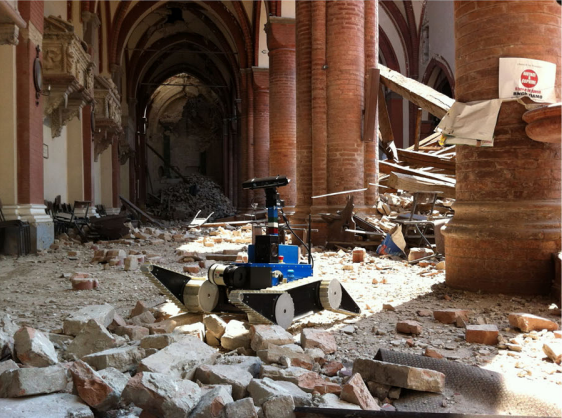
\includegraphics[width=0.35\textwidth]{stateof-tracked}
	\caption{A tracked USAR robot, with paddles for obstacle climbing \citep{stateof}.}
	\label{stateof tracked}
\end{wrapfigure}

In both natural and man-made disasters, USAR operations are critical for reducing casualties. Robots can be deployed in USAR operations to complement human and canine rescuers. Robots have the advantage of being able to be deployed in scenarios too small or too dangerous for humans, and aerial robots such as quadcopters are extremely effective at quickly mapping terrain and providing situational awareness to teams. Other emerging applications of USAR robotics are remote fire fighting, victim interaction, and extraction \citep{stateof}.\\
\begin{wrapfigure}{l}{0.35\textwidth} %this figure will be at the left
	\centering
	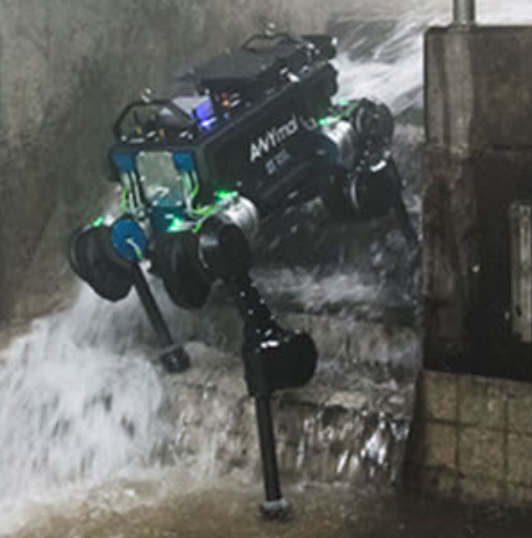
\includegraphics[width=0.35\textwidth]{stateof-wheelleg}
	\caption{ANYmal, a legged USAR robot \citep{stateof}.}
	\label{stateof wheelleg}
\end{wrapfigure}

In order to perform USAR operations, robots need some form of locomotion. For ground robots, this typically involves either tracks, wheels, or legs. \citep{stateof}. Tracked robots with actuated paddles for obstacle climbing, such as the one shown in Figure \ref{stateof tracked}, have been found to perform extremely well. This is evident by their representation in the winners of the Robocup Rescue Robot League (RRL), an event in which teams compete to produce robots for versatile USAR operations \citep{Sheh-2016}. Wheeled robots are generally the simplest and easiest to repair, but can get stuck more easily in uneven terrain. Legged robots provide the advantage of not needing a continuous path, and rapid developments in optical sensors and control systems are enabling them to be even more viable. Wheel-leg hybrid systems will use legged motion for navigating difficult terrain, and wheels when on smooth ground \citep{stateof}. 
\newpage
\section{Load-Intuitive Modules} %~~~~~~~~~~~~~~~~~~~~~~~~~~~~~~~~~~~~~~~~~~~~~~~~~~~~~~~~~~~~~~

\begin{wrapfigure}{r}{0.35\textwidth} %this figure will be at the right
	\centering
	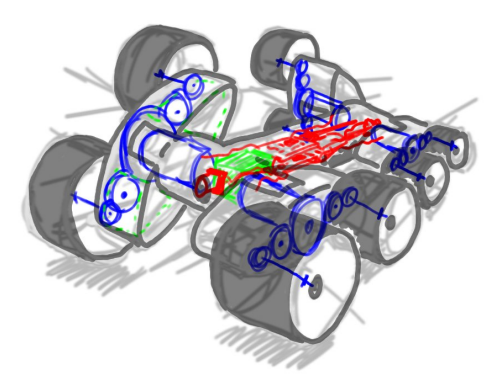
\includegraphics[width=0.35\textwidth]{Wilson-sketch}
	\caption{Systems layout of Wilson's LIM device \citep{Wilson-2013}.}
	\label{Wilson sketch-lit}
\end{wrapfigure}

A Load-Intuitive Module (LIM) refers to a wheel system proposed by Matthew Wilson, shown in Figure \ref{Wilson sketch-lit} \citep{Wilson-2013}. The LIM system uses a two outer "minor wheels" placed on a central hub that can be rotated as a "major wheel". The minor wheels are geared to the central hub such that they drive the vehicle, however if they experience high resistance, for example from hitting an obstacle, the torque will cause the major wheel to rotate instead, flipping one of the minor wheels over the obstacle to automatically climb it. The system is referred to as "Load-Intuitive" because it will intuitively climb over obstacles in response to increased load on the wheels. LIMs are designed to be used in low cost USAR robots, allowing them to climb over objects without the need for many actuators.\\

One advantage LIMs provide over existing locomotion methods is that they can climb obstacles higher than their profile, meaning they can enter low voids while rolling, and climb relatively tall obstacles by flipping over them. Another advantage is that LIMs require minimal actuation, one motor can be used to drive both the rolling and flipping motion, which will reduce costs when compared with other designs.\\

\noindent "LIMed" robot platforms (platforms using LIMs for locomotion) were built individually by four final year students at UCT \citep{Wilson-2013}, \citep{Haskel-2017}, \citep{Buchanan-2018}, and \citep{Powrie-2019}. These platforms show some success in climbing a single step, albeit inconsistently.

\subsection{Wilson's LIM robot} %~~~~~~~~~~~~~~~~~~~~~~~~~~~~~~~~~~~~~~~~~~~~~~~~~~~~~~~~~~~~~~~~~~~~~~~~~~~~~~~~

\begin{wrapfigure}{r}{0.35\textwidth}
	\centering
	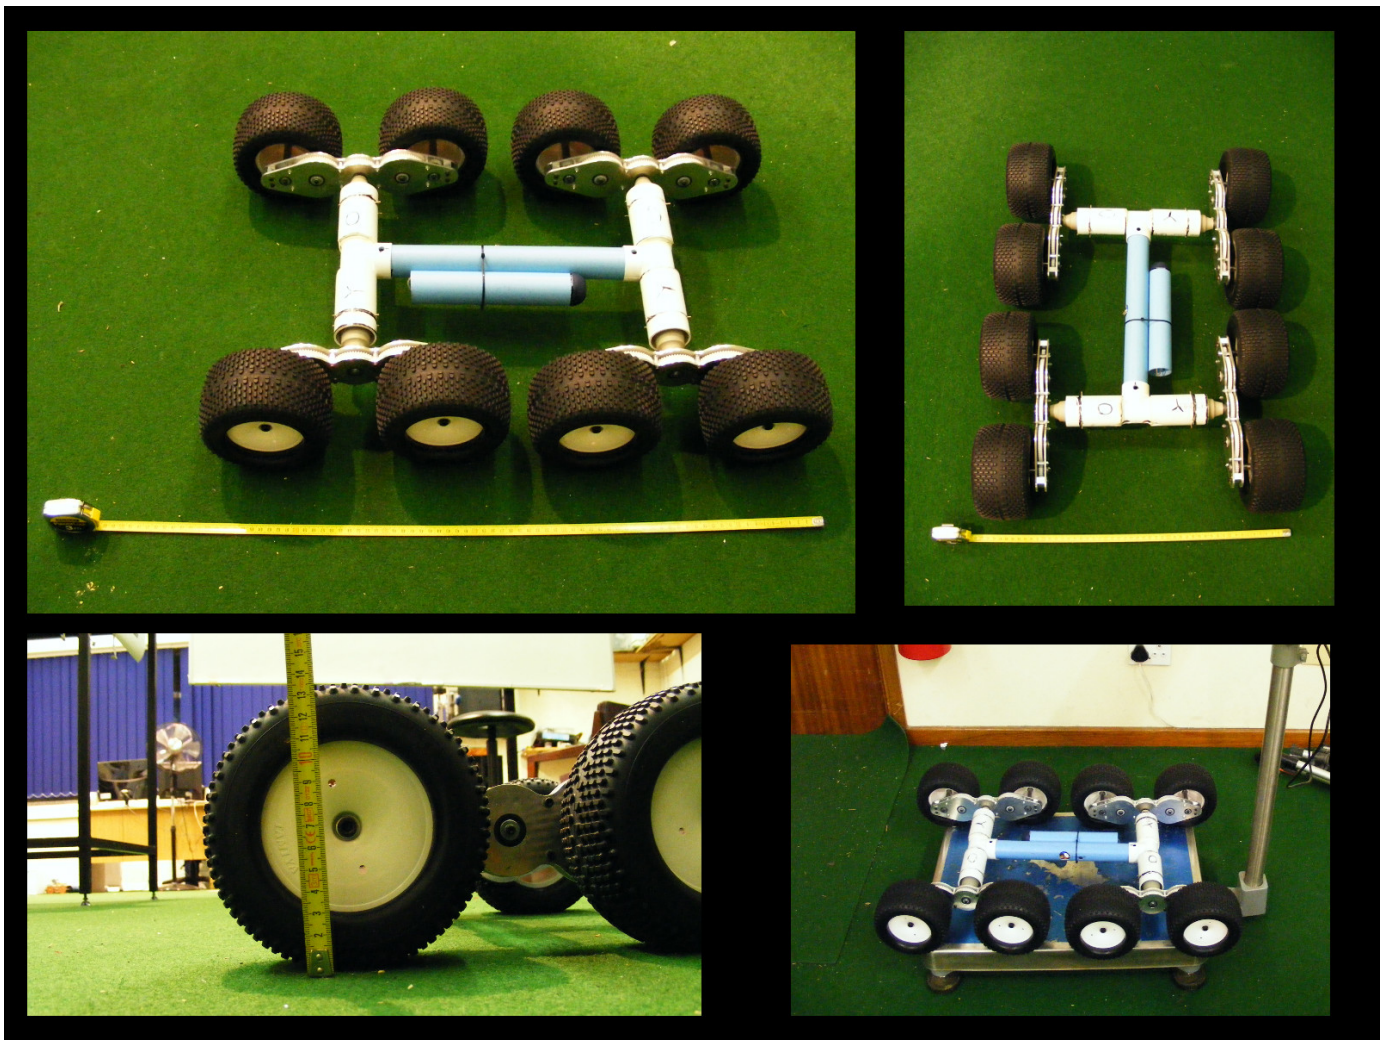
\includegraphics[width=0.35\textwidth]{Wilson-robot}
	\caption{Wilson's Robot \citep{Wilson-2013}.}
	\label{Wilson robot}
\end{wrapfigure}

Wilson designed and built the first LIM robot in 2013, shown in Figure \ref{Wilson robot}. This robot was designed as a prototype for a low cost USAR stair-climbing robot. At first Wilson considered only using LIMs for the front set of wheels, with the rear set using regular wheels. However, after performing a 2D simulation in Algodoo, he concluded that using LIMs for the rear wheels was necessary as regular wheels provided little to no support to the climbing motion after the first step, presumably because the rear wheel would stop making contact with the stairs. Using LIMs for the rear wheels means they will be able to climb as well, and can always apply a forward force on the body.



\begin{wrapfigure}{l}{0.35\textwidth}
	\centering
	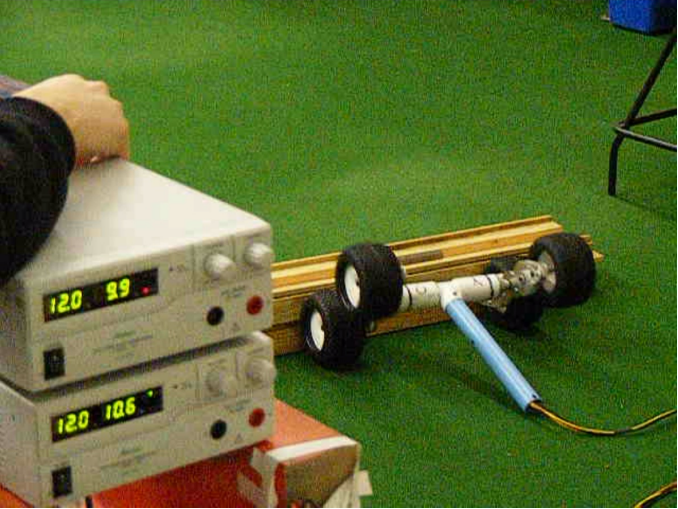
\includegraphics[width=0.35\textwidth]{Wilson-climbing}
	\caption{Wilson's half assembly climbing a stair \citep{Wilson-2013}.}
	\label{Wilson climbing}
\end{wrapfigure}

Wilson's robot had some limitations that prevented him from performing extensive tests. Chiefly, it was unable to climb stairs as the motors would stall upon encountering an obstacle. To validate the LIM concept in spite of this issue, Wilson split the robot in half and tested stair climbing using only the front LIMs and the chassis dragging behind as a tail. This "tail-dragging half assembly" was able to climb a single step as shown in Figure \ref{Wilson climbing}. Wilson's project ran out of time before he was able to solve the climbing motion of the complete robot, however he was able to confirm that the LIM system can climb at least a single stair in the half assembly configuration \citep{Wilson-2013}.

\subsection{Haskel's Theseus} %~~~~~~~~~~~~~~~~~~~~~~~~~~~~~~~~~~~~~~~~~~~~~~~~~~~~~~~~~~~~~~~~~

\begin{wrapfigure}{r}{0.35\textwidth}
	\centering
	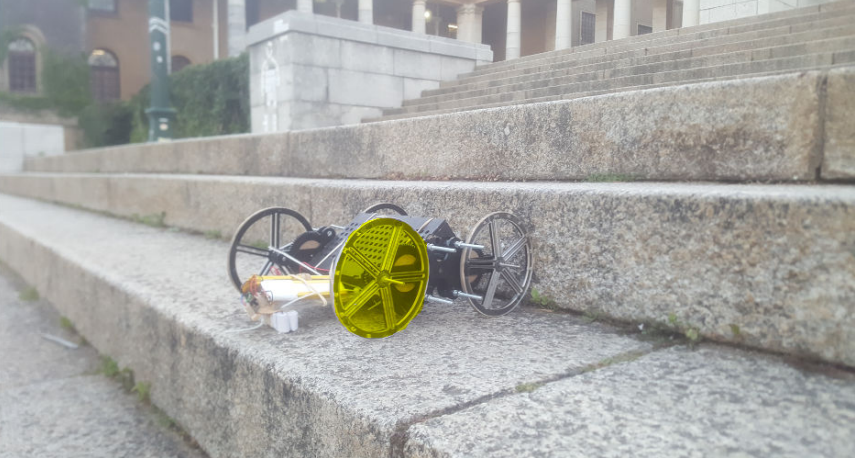
\includegraphics[width=0.35\textwidth]{Haskel-robot}
	\caption{Haskel's Theseus \citep{Haskel-2017}.}
	\label{Haskel robot}
\end{wrapfigure}
Haskel designed and built a LIMed robot to further test the concept, which he named "Theseus", shown in Figure \ref{Haskel robot}. Unlike Wilson, Haskel assumes that using LIMs for rear wheels is not necessary for the stair climbing motion, and instead chooses to use a dragging tail to provide counter torque, similar to the tail-dragging half assembly used by Wilson. Theseus is much smaller and lighter than Wilson's robot.\\

Haskel tested different concepts for the tire tread, dragging tail, and gear ratios. However, none of his configurations could consistently climb a step. In the majority of step-climbing attempts, Theseus' LIMs would flip over to mount the step, but it would not be able to pull itself up. This can be attributed to a lack of grip or a lack of torque. Haskel intended to do further work on the project, however he ran out of time due to component shortages and protests at UCT \citep{Haskel-2017}.
\newpage
\subsection{Buchanan's Ascender} %~~~~~~~~~~~~~~~~~~~~~~~~~~~~~~~~~~~~~~~~~~~~~~~~~~~~~~~~~~~~~~~~~

\begin{wrapfigure}{r}{0.35\textwidth}
	\centering
	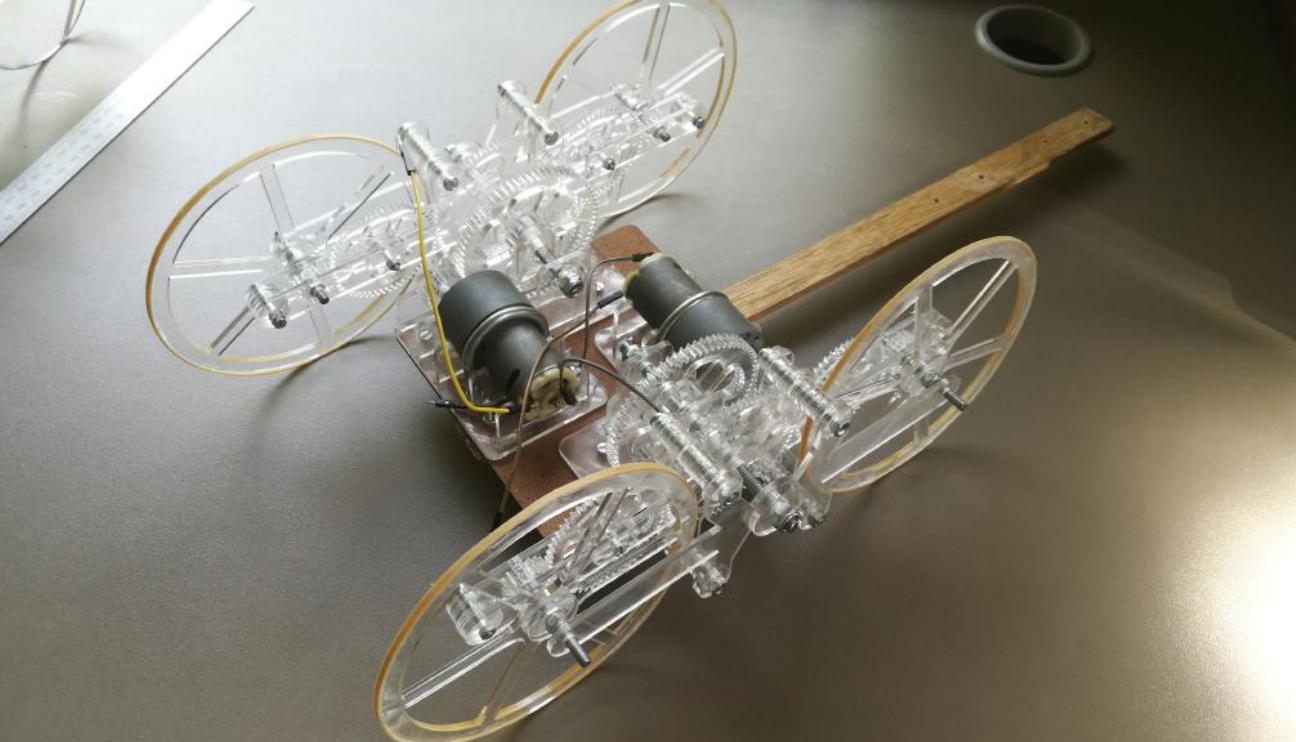
\includegraphics[width=0.35\textwidth]{Buch-robot}
	\caption{Buchanan's Ascender \citep{Buchanan-2018}.}
	\label{Buch robot}
\end{wrapfigure}
Buchanan designed and built "Ascender", a robot platform using LIMs for locomotion, shown in Figure \ref{Buch robot}. Buchanan iterated on the design several times in order to reduce mass and increase torque. The intention was to build a drivetrain that could be combined with the electronics of Haskel's Theseus to produce a successful stair climbing robot. As such, the Ascender does not include any electronic control systems, and is instead controlled externally by power supplies connected to the motors.

Buchanan's testing showed that the Ascender was able to climb a single step of 120 mm in 6 out of 10 attempts, and a step of 140mm in 2 out of 10 attempts. Buchanan noted a flaw in the design; after the LIMs flip over as part of the climbing motion, the body of the robot would lodge itself onto the edge of the step and the wheels would spin freely, a phenomenon referred to as beaching. The LIMs would then spin until the top wheel makes contact with the top of the step, from there it would either grip and pull the robot up the step as intended, or it would dislodge the body and the robot would fall off the step. Buchanan also reported that the Ascender was fragile to the point that it broke during the testing. Buchanan did not test the Ascender's ability to climb a staircase, but he concluded that it would be able to as a staircase is simply repeated single steps. \citep{Buchanan-2018}

\subsection{Powrie's Di-Wheel robot}

\begin{wrapfigure}{r}{0.35\textwidth}
	\centering
	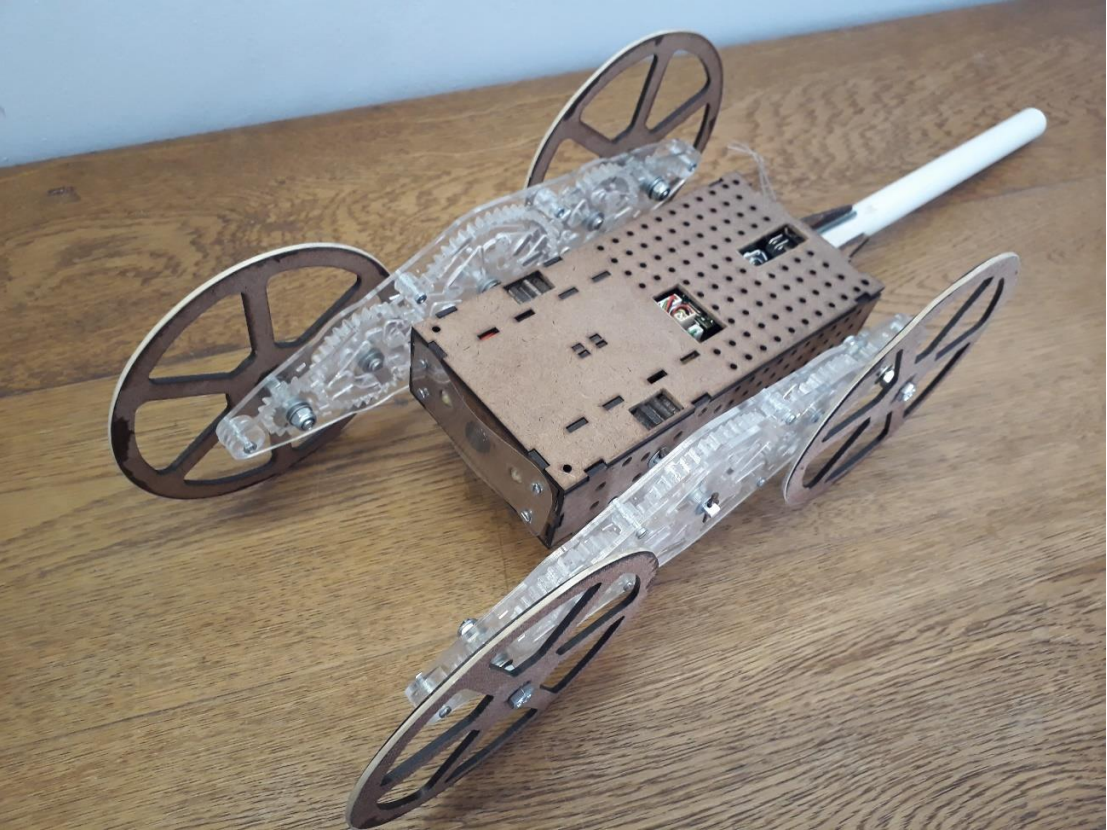
\includegraphics[width=0.35\textwidth]{Powrie-device}
	\caption{Powrie's Di-Wheel Robot \citep{Powrie-2019}.}
	\label{fig:Powrie robot}
\end{wrapfigure}
Powrie developed a robot using LIMs, however in his report he referred to LIMs as Di-Wheels. His reason for renaming them is that the behaviour of the LIMs does not only respond to external loads on the wheels, it also depends on the torque applied by the motors. He chose the name "Di-Wheel" in reference to a similar design by the name of "Tri-Wheel", which used three minor wheels instead of two, developed by \cite{Smith-2015}. Powrie's Di-Wheel robot is larger and more robust than Buchanan's Ascender, while being lighter than Wilson's LIMed robot. It is shown in Figure \ref{fig:Powrie robot}.\\


The Di-Wheel robot was successful in climbing a single step of 220 mm. Further testing was not performed as noise from the robot's motors would interfere with the control system, preventing untethered driving. Powrie ran out of time before he was able to solve this issue. Powrie also found that when both motors are powered on, one of the LIMs would flip first, putting all the weight on the other LIM so preventing it from flipping. The result is that the robot would fall on its side, as seen in Figure \ref{Powrie falling} \citep{Powrie-2019}.\\
\begin{figure}[ht]
	\centering
	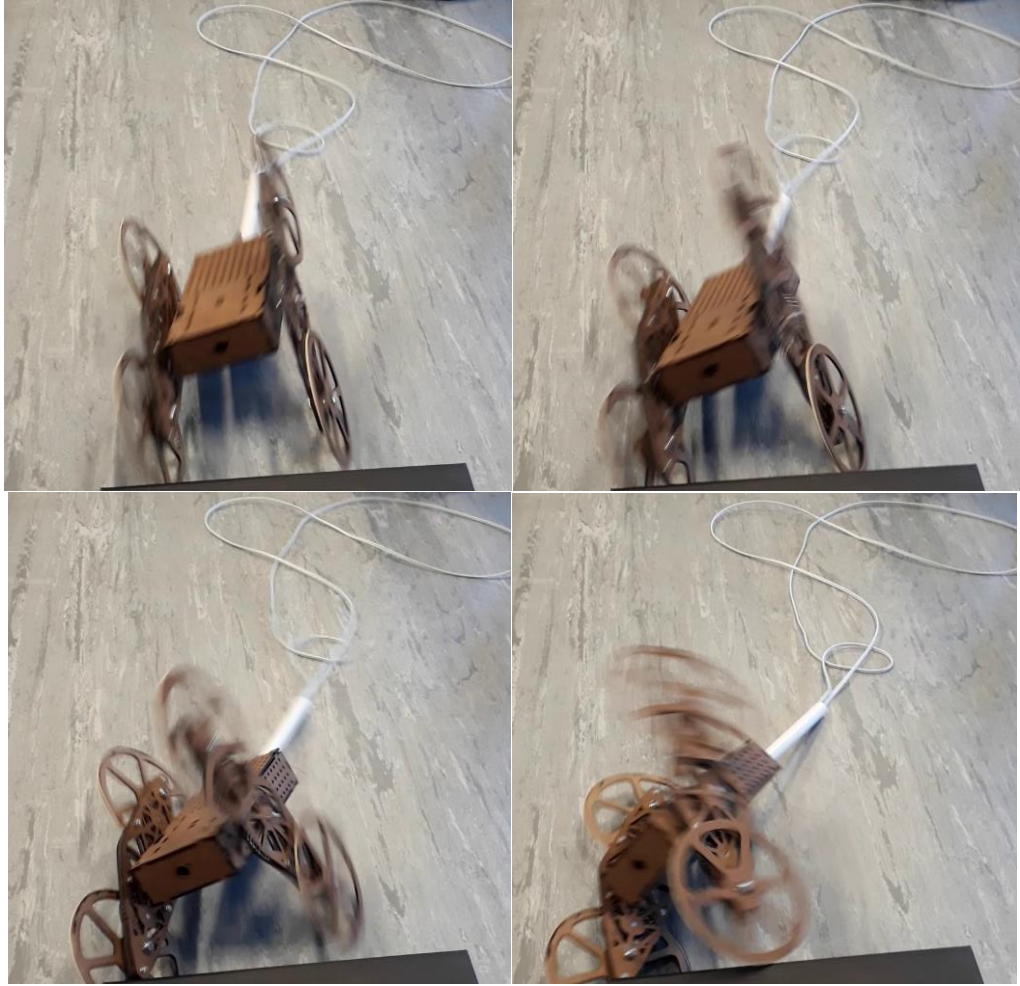
\includegraphics[width=0.5\textwidth]{Powrie-falling}
	\caption{The Di-Wheel robot falling due to unsynchronised LIMs \citep{Powrie-2019}.}
	\label{Powrie falling}
\end{figure}


\subsection{Gearing} %~~~~~~~~~~~~~~~~~~~~~~~~~~~~~~~~~~~~~~~~~~~~~~~~~~~~~~~~~~~~~~~~~
%Add drawing!!
The gear ratios of the LIMs will affect its motion significantly. The rotational speed of the central gear will be translated into both the speed of the LIM frame and the speed of the wheels:
\begin{align*}
	\dot{\theta}_{\mathrm{Sun}} &= \dot{\theta}_{\mathrm{Frame}} + \frac{N_\mathrm{Planet}}{N_\mathrm{Sun}}\dot{\theta}_{\mathrm{Planet}} \tag{1}\\
\end{align*}
where $\dot{\theta}_{\mathrm{Sun}}$ is the angular speed of the central gear, $\dot{\theta}_{\mathrm{Frame}}$ is the angular speed of the LIM frame, $\dot{\theta}_{\mathrm{Planet}}$ is the angular speed of the outer gears and wheels relative to the frame, $N_{\mathrm{Planet}}$ is the number of teeth on the outer gears, and $N_\mathrm{Sun}$ is the number of teeth on the central gear.\\

When both the wheels and the LIM frame aren't constrained, the system is under-actuated and its motion is non-trivial. In the case that the LIM frame isn't flipping (i.e. normal driving on a flat plane), $\dot{\theta}_{\mathrm{Frame}} = 0$, therefore:\\
 \begin{align*}
 	\dot{\theta}_{\mathrm{Planet}} &= \frac{N_\mathrm{Sun}}{N_\mathrm{Planet}}\dot{\theta}_{\mathrm{Sun}} \tag{2}\\
 \end{align*}
When the wheels have encountered an obstacle, such as a step, friction will prevent them from turning, $\dot{\theta}_{\mathrm{Planet}} + \dot{\theta}_{\mathrm{Frame}} = 0$. In this case:
\begin{align*}
	\dot{\theta}_{\mathrm{Frame}} &= \frac{\dot{\theta}_{\mathrm{Sun}}}{(1-\frac{N_\mathrm{Planet}}{N_\mathrm{Sun}})} \tag{3}\\
\end{align*}

This means that during flipping motion, if $\frac{N_\mathrm{Planet}}{N_\mathrm{Sun}} > 1$, then the LIM frame will flip in the opposite direction to the rotation of the central gear, so the front wheel will roll up the side of the obstacle \citep{Wilson-2013}. This is ineffective for climbing steps as the LIM will never mount the step, but rather continue rotating backwards until it returns to the starting position \citep{Haskel-2017}.\\

\begin{figure}[h]
	\centering
	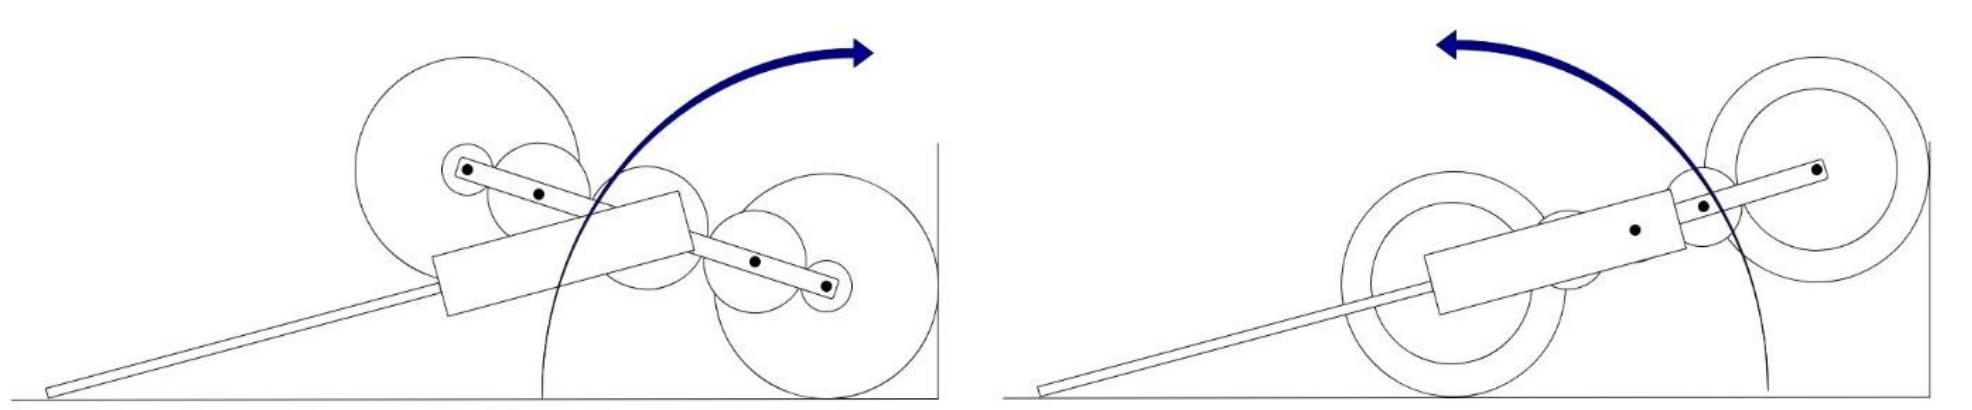
\includegraphics[width=0.9\textwidth]{Powrie-gear-differences}
	\caption{Two different climbing motions using different gear ratios \citep{Powrie-2019}.}
	\label{Powrie gears}
\end{figure}

If $\frac{N_\mathrm{Planet}}{N_\mathrm{Sun}} < 1$, then the LIM frame will rotate forward, the rear wheel will flip over and mount the obstacle. This allows the LIM to climb stairs as intended.\\
The two cases are shown in Figure \ref{Powrie gears}, with the left showing the case when $\frac{N_\mathrm{Planet}}{N_\mathrm{Sun}} < 1$, and the right showing the case when $\frac{N_\mathrm{Planet}}{N_\mathrm{Sun}} > 1$.



%\subsection{Control requirements} %~~~~~~~~~~~~~~~~~~~~~~~~~~~~~~~~~~~~~~~~~~~~~~~~~~~~~~~~~~~~~~~~~
%
%LIMs are considered "Load intuitive" because of their ability to adapt to terrain mechanically. Open-loop control is ideal in this case, as an operator need only turn the motor on and the LIM will drive forward if it can, or attempt to climb an obstacle if it is obstructed \citep{Wilson-2013}. However, Powrie found that his robot was not suited to open loop control. When full voltage is provided to the motor, the LIMs would flip even if when is on a flat plane. Powrie's calculations suggest that whether the LIM flips or not is largely dependent on the torque applied to it. A low torque results rolling, and a high torque results in flipping. His report suggests that LIMs only responds to terrain intuitively for a "medium torque" \citep{Powrie-2019}. In this case a medium torque would be defined as a torque that results in rolling when the LIM is unobstructed, and flipping only when it is obstructed. This indicates that it may be necessary to have a control system that manages the torque provided to the LIMs to ensure that they do not flip on flat terrain if the motors are sufficiently powerful.\\
%
%Powrie also found that when climbing a step, one LIM could flip first, putting weight on the other and preventing it from flipping, as seen previously in Figure \ref{Powrie falling} \citep{Powrie-2019}. This suggest that a control system is needed to roughly synchronise the LIMs, if one is ahead of the other, more torque should be provided to the trailing LIM to correct its motion.
\chapter{2D simulation}

In order to create an accurate model of the LIM system, it is important to understand how it functions. Previous reports have given some insight into this, but none of them have demonstrated a LIM robot that can climb consecutive steps. Wilson performed a simple simulation of a LIM robot in Algodoo, and concluded that the robot would need LIMs for the rear wheels in order to support consecutive stair climbing \citep{Wilson-2013}, however all of the subsequent projects simply used a dragging tail instead of rear wheels. There is a need to resolve this inconsistency in past work, and to gain insight into the function of the LIM system. To do this, another 2D simulation using Algodoo is performed.

\section{Limitations}

Algodoo is a two dimensional physics sandbox \citep{Algodoo}. Initial testing with the software showed that limitations on the physics engine prevent accurate simulation of gears with teeth at a centimetre scale. This means it is impossible to accurately simulate a LIM device at the scale that they would be used in reality. The simulation can be scaled up to avoid this issue. However, this prevents an accurate simulation of the kinematics of the system.\\

Additionally, it was found that Algodoo does not allow for the accurate simulation of an electric motor. In a typical electric motor, the available torque will decrease as the speed increases. This nuance is not present in Algodoo, so it cannot be used to provide an accurate simulation of the motor requirements. Despite these limitations. Algodoo is still useful as a tool to roughly test the motion of LIMs, and to determine how it would interact with steps. The advantage of Algodoo over other simulation methods is its ease of use, it only takes a few minutes to build a LIMed robot in Algodoo.

\section{Configuration}


To improve the accuracy of the Algodoo physics engine, the simulation frequency is set to 1200 and all objects are scaled up 100 times. A basic LIM system with a dragging tail is set up, using gear and wheel dimensions from \cite{Powrie-2019}, shown in Figure \ref{algo-model}.

\begin{figure}[h]
	\centering
	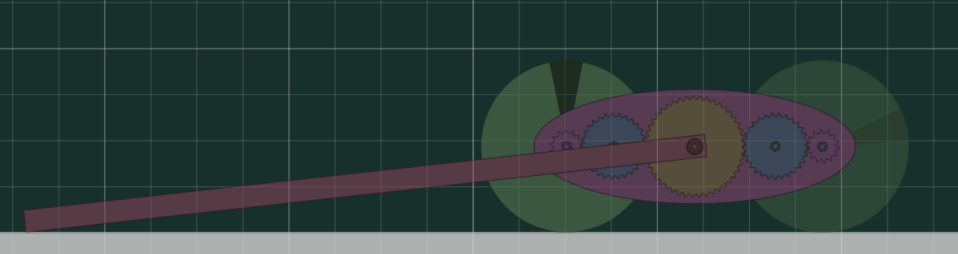
\includegraphics[width=0.8\textwidth]{algo-model}
	\caption{Initial Algodoo LIM system}
	\label{algo-model}
\end{figure}
\section{Observations}

\subsection{Rear wheels}

Simulations suggest that rear wheels are not necessary for successful consecutive stair climbing. If the motor torque is sufficient, the LIM will be able to climb steps with only a dragging tail for counter torque. It should be noted that adding a motorised rear wheel, with or without LIMs, does provide a supporting force to the front LIMs during flipping motion, so if the frontal motor cannot provide sufficient torque, rear wheels should be considered in the design.

\subsection{Mounting obstacles}

There are three ways in which a LIM can mount an obstacle after flipping up to it. The first is that the wheel collides directly with the obstacle, shown in Figure \ref{algo-case-wheel}. This happens when the obstacle is taller than a certain threshold based on the geometry of the LIM, and can result in the wheel bouncing off of the obstacle and failing to pull itself up. In this case a controller may be used to limit the speed of the flipping motion to ensure that the wheel is not going fast enough to bounce off the obstacle when it collides. \\

\begin{figure}[h]
	\centering
	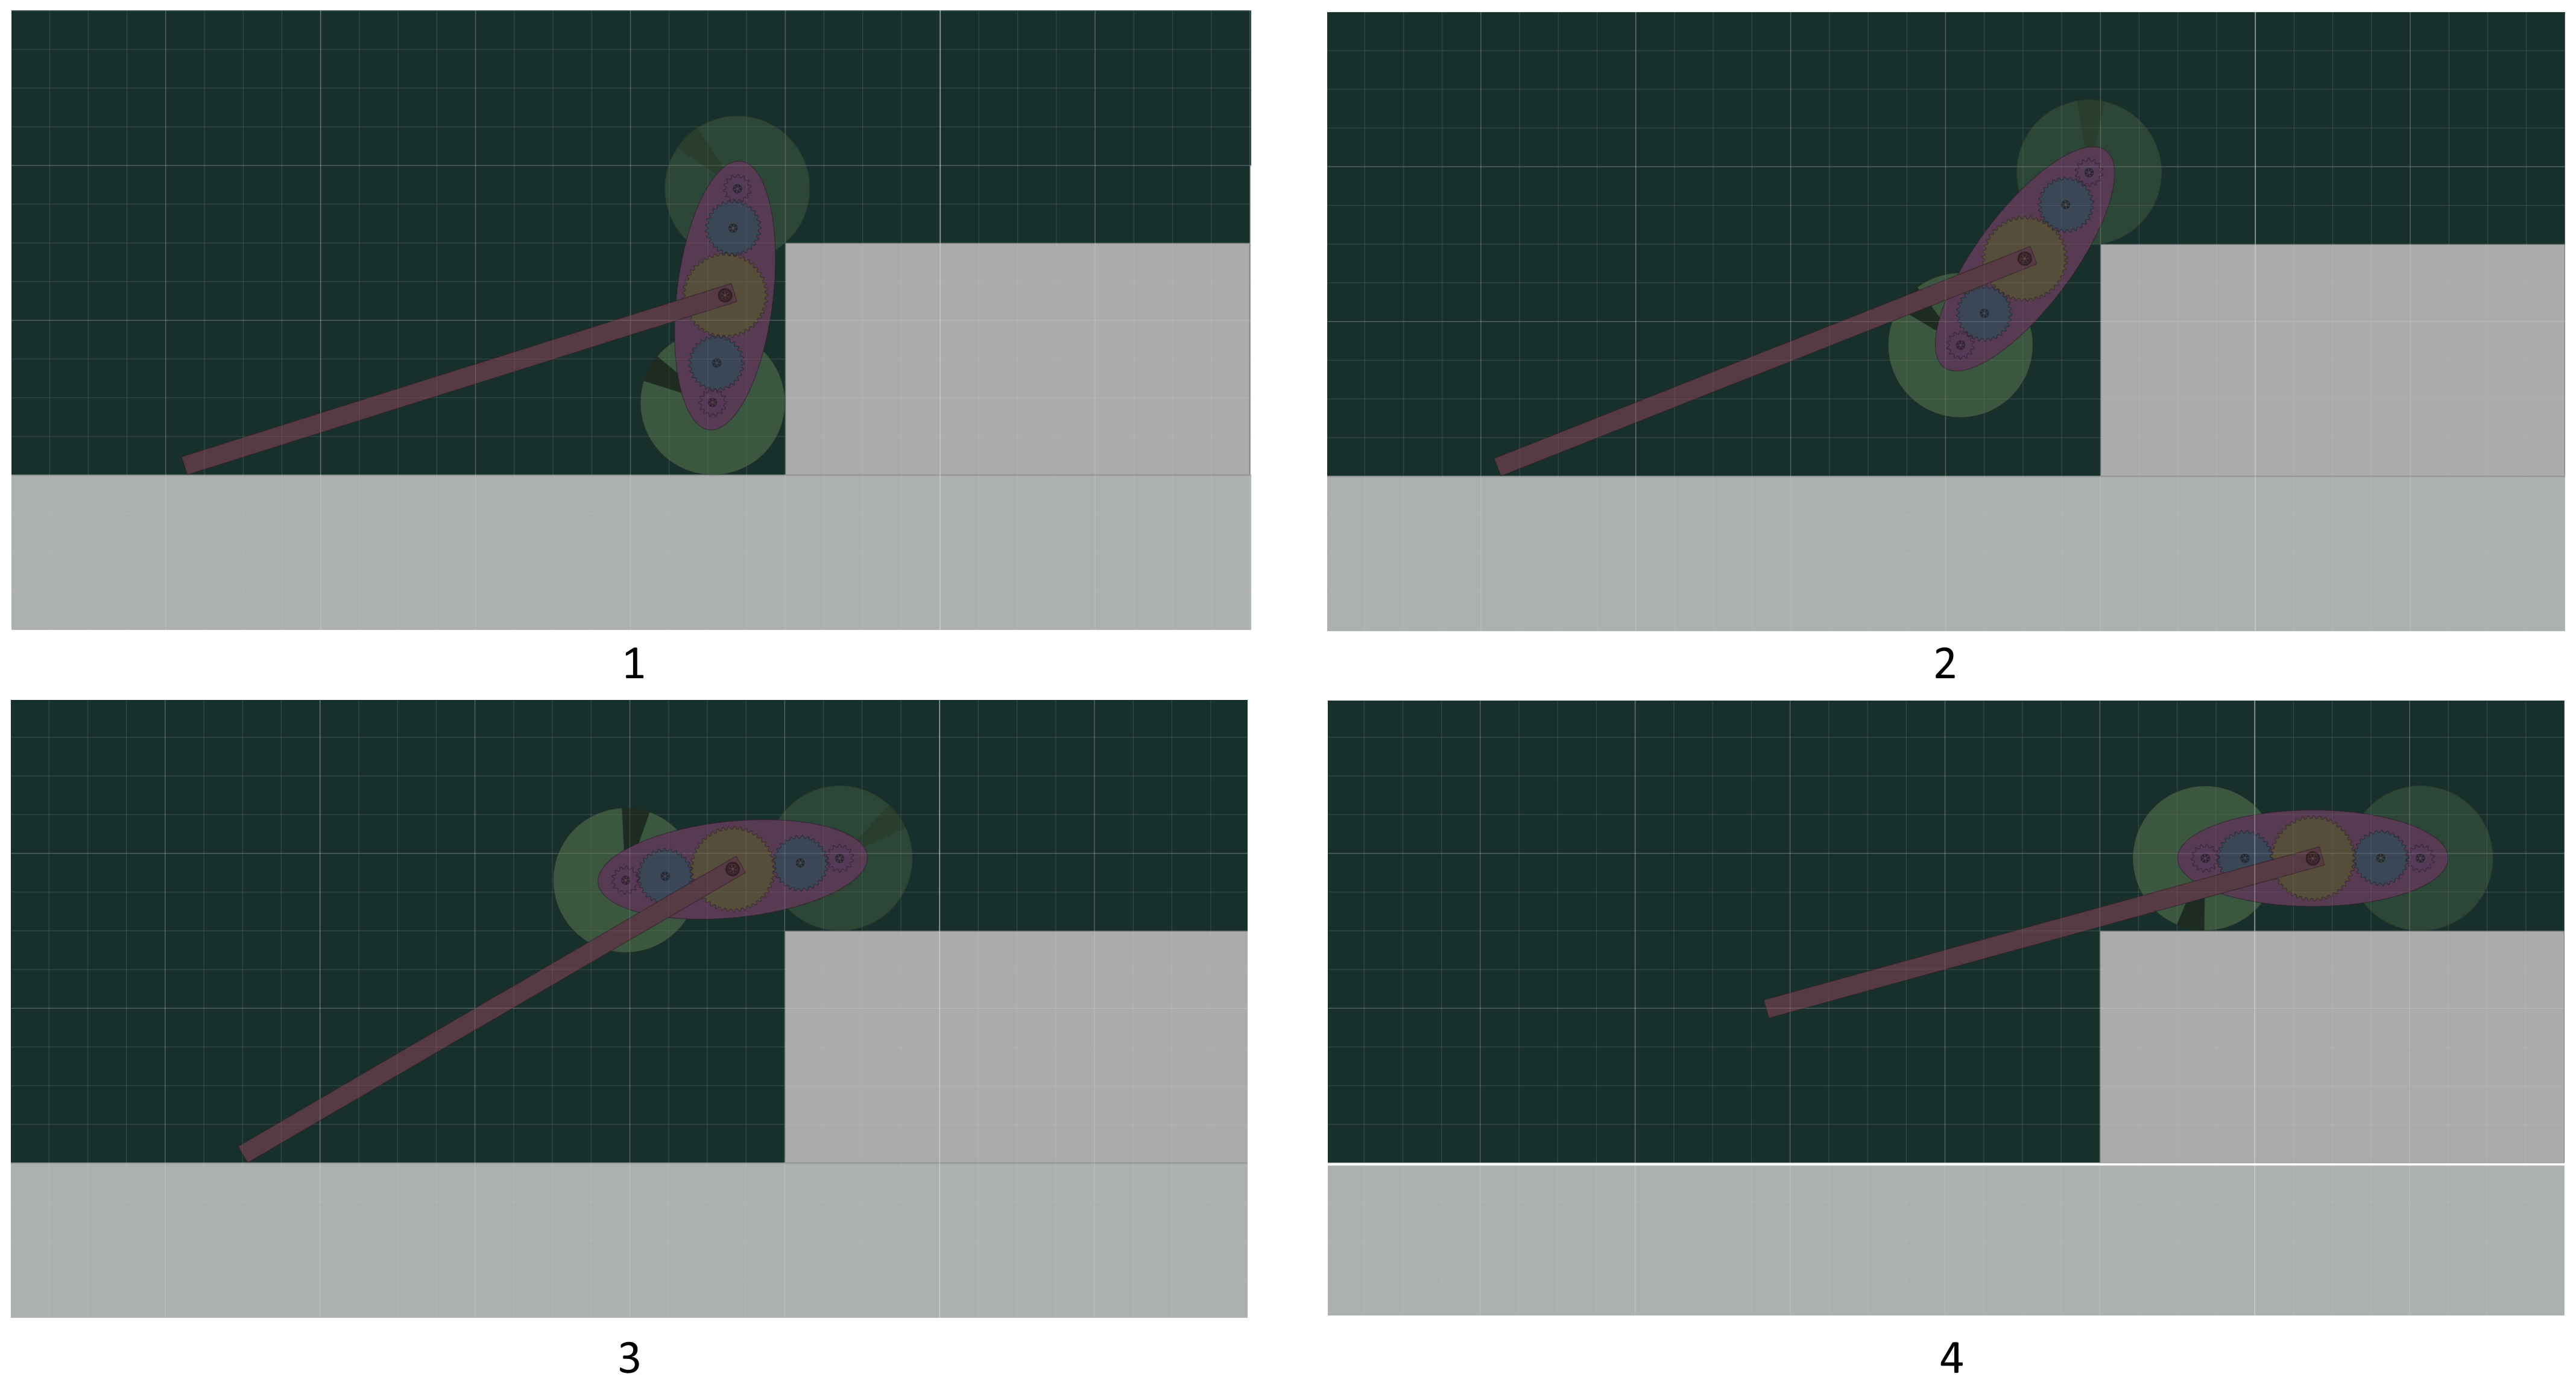
\includegraphics[width=0.8\textwidth]{algo-case-wheel}
	\caption{LIM climbing with wheel contact}
	\label{algo-case-wheel}
\end{figure}

The second way is that the LIM frame collides with the obstacle and mounts it, then the LIM continues to rotate until the wheel makes contact with the surface of the obstacle to pull the robot forward. This case is shown in Figure \ref{algo-case-frame}. Note that the LIM frame can slip on the edge of the obstacle, which may result in failure to climb. \\

\begin{figure}[h]
	\centering
	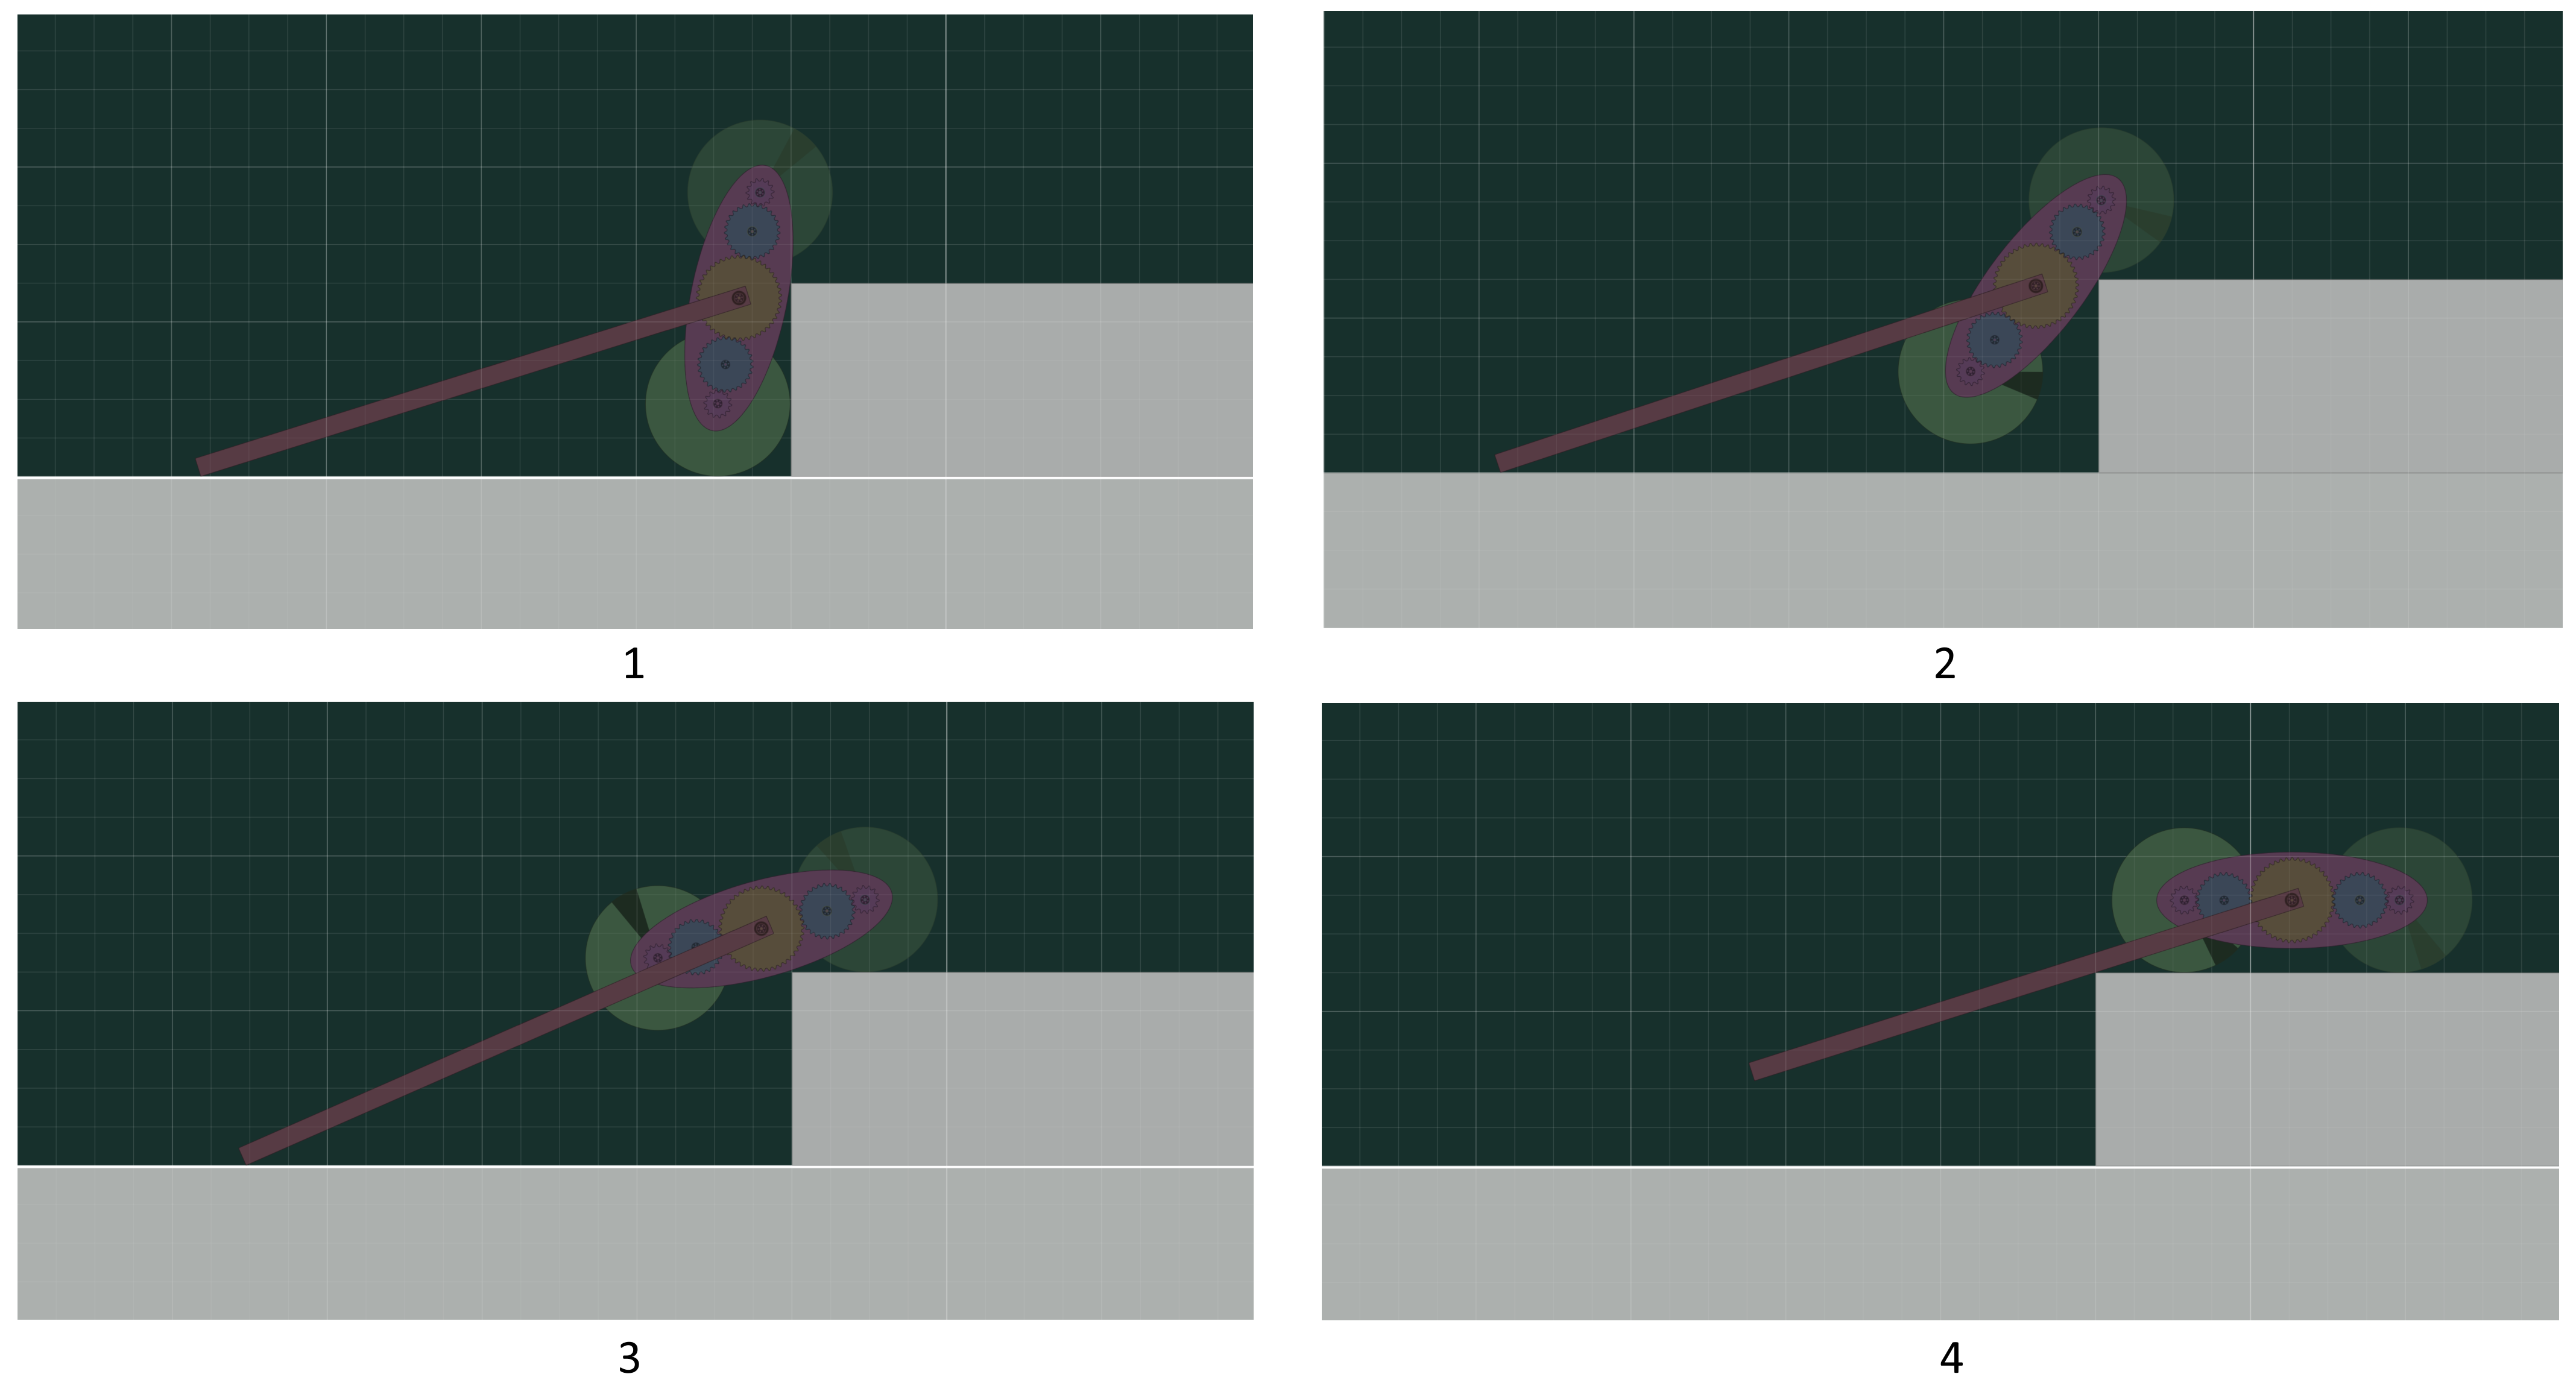
\includegraphics[width=0.8\textwidth]{algo-case-frame}
	\caption{LIM climbing with LIM frame contact, note how the contact point slips between 1 and 2}
	\label{algo-case-frame}
\end{figure}

The third way is that the body of the robot, presented here as an extension of the tail, will mount the obstacle. This is shown in Figure \ref{algo-case-body}. When the body has beached onto the obstacle, seen in Figure \ref{algo-case-body}.2, there is nothing resisting the motion of either the wheels or the LIM, so they can accelerate quite quickly. If they move too fast, the wheel can bounce off the obstacle when it makes contact, dislodging the body so that it falls back down to the initial position. \cite{Buchanan-2018} found that his Ascender followed this motion, which caused it to fail many of its climbing tests. He mentions that this can be avoided by moving the LIM axle to the end of the body, so that the body does not protrude beyond the LIM frame during climbing motion.\\

\begin{figure}[h]
	\centering
	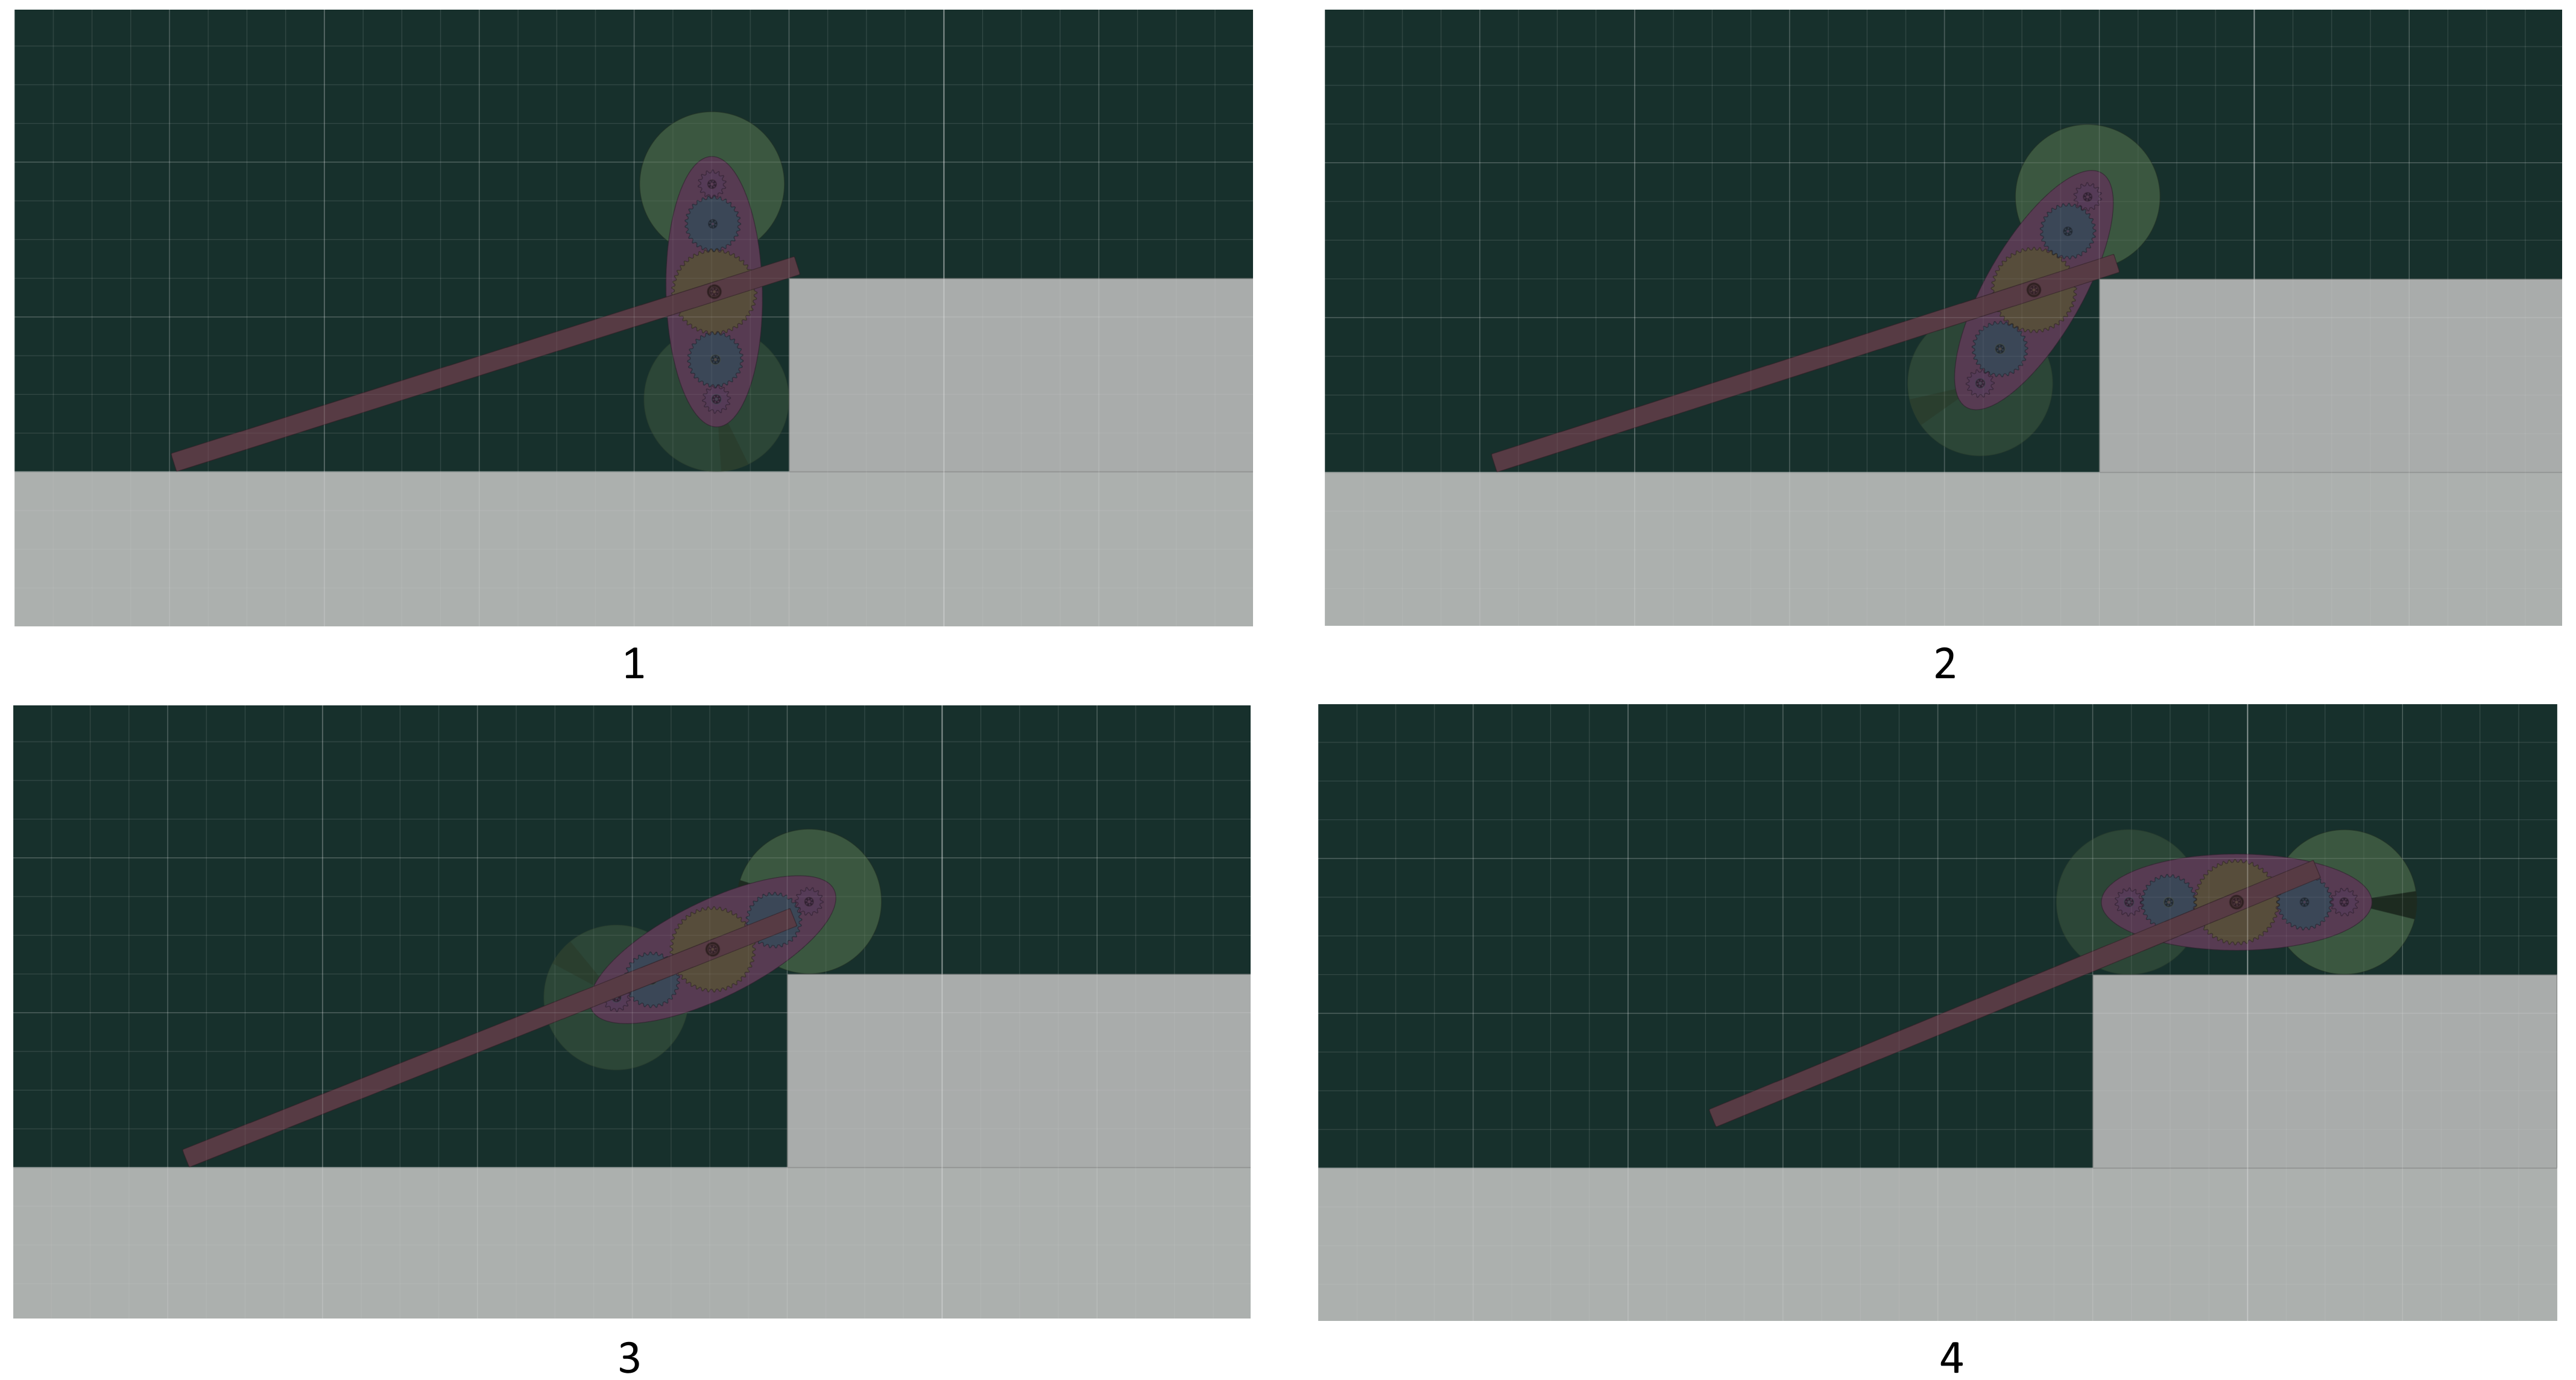
\includegraphics[width=0.8\textwidth]{algo-case-body}
	\caption{LIM climbing with robot body contact}
	\label{algo-case-body}
\end{figure}

Each of these climbing methods has its flaws, however the case where the LIM frame collides with the obstacle is preferred as it reduces the chance that the wheel will bounce off the obstacle. To address slipping, grousers can be added to the robot's body \citep{rob2014}. The updated model with grousers can be seen in Figure \ref{algo-model2}.\\

\begin{figure}[h]
	\centering
	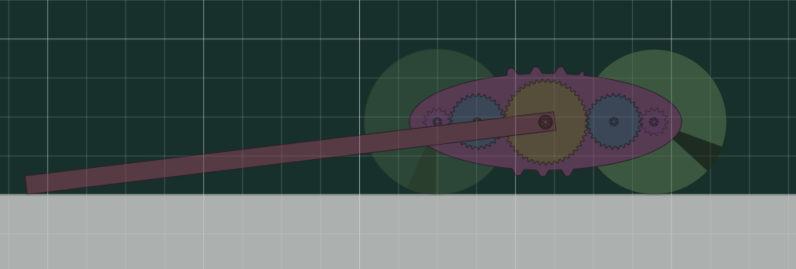
\includegraphics[width=0.8\textwidth]{algo-model2}
	\caption{Algodoo LIM system with grousers on frame}
	\label{algo-model2}
\end{figure}

\subsection{Rolling and flipping}

It was observed in simulation that the LIM would either roll or flip depending on the torque applied to it. There appeared to be a very small range of "medium torque" at which the LIM was truly load intuitive, if the motor torque was too weak it would never be able to flip over the obstacle and if it was too strong it would always flip and never roll, which hinders movement on flat terrain. However, this may simply be a result of inaccuracies of the simulation, as scaling and poor motor physics could significantly affect this motion. \\

In reality, as an electric motor increases in speed, the torque available will decrease proportionally. This means that once the LIM is rolling at speed, it will no longer have enough torque to flip itself unless it is stopped by an obstacle. This suggests that too much torque will only cause unintended flipping when the LIM is at rest on a flat plane.\\

\begin{figure}[h]
	\centering
	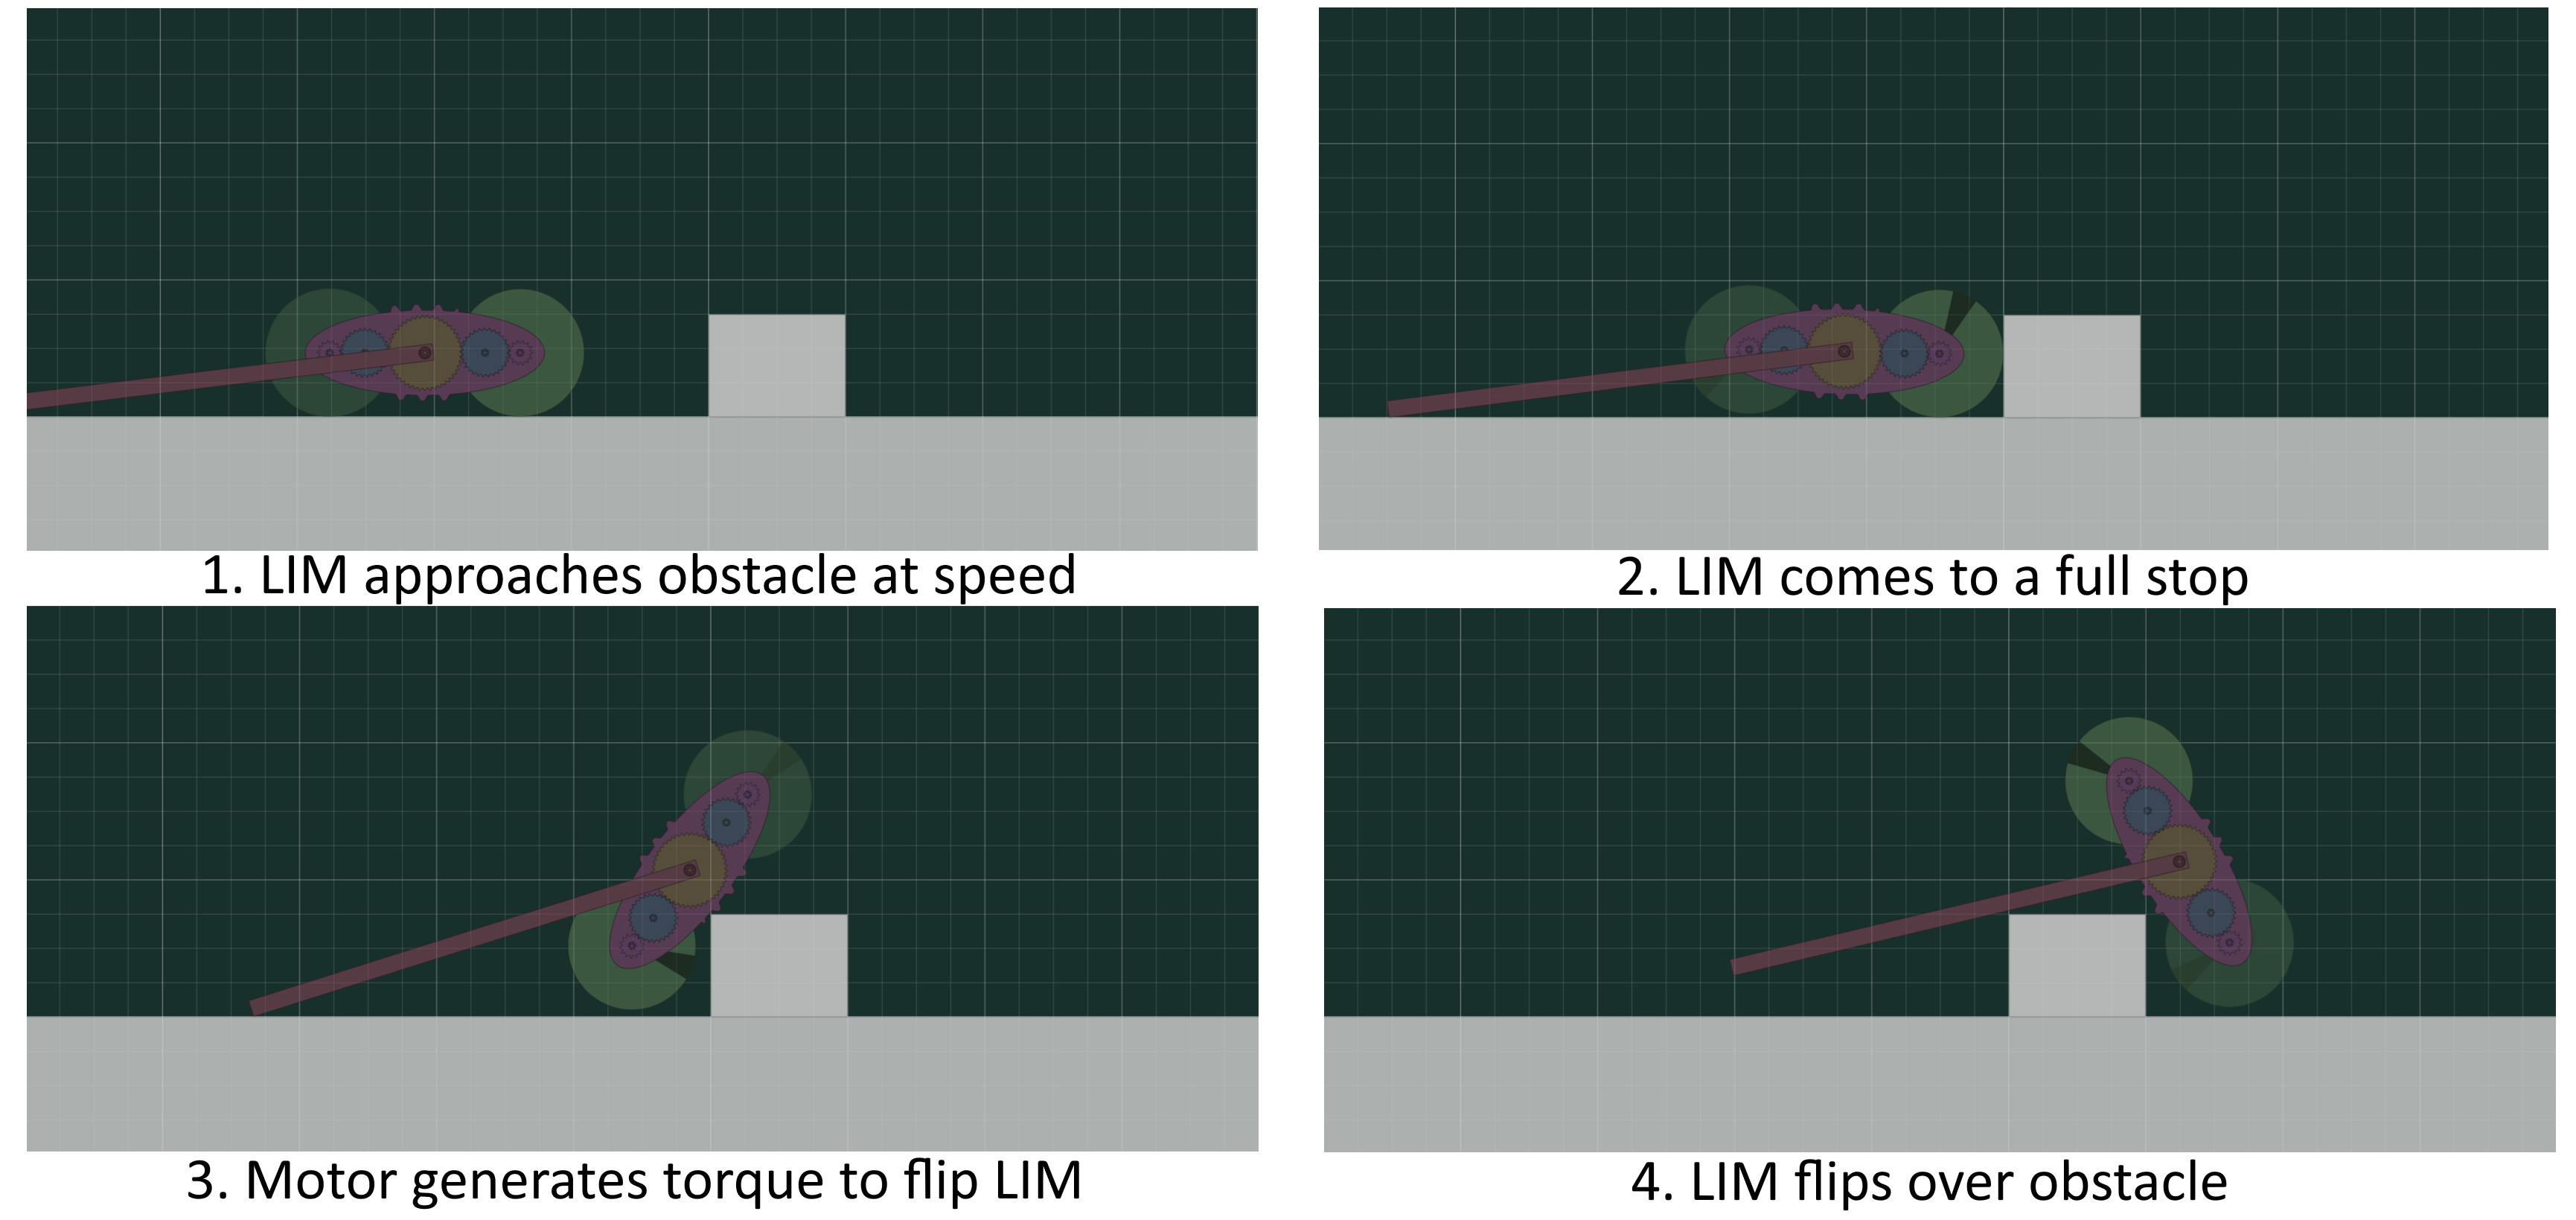
\includegraphics[width=1\textwidth]{algo-hori}
	\caption{Algodoo LIM system approaching obstacle horizontally}
	\label{algo-hori}
\end{figure}

\begin{figure}[h]
	\centering
	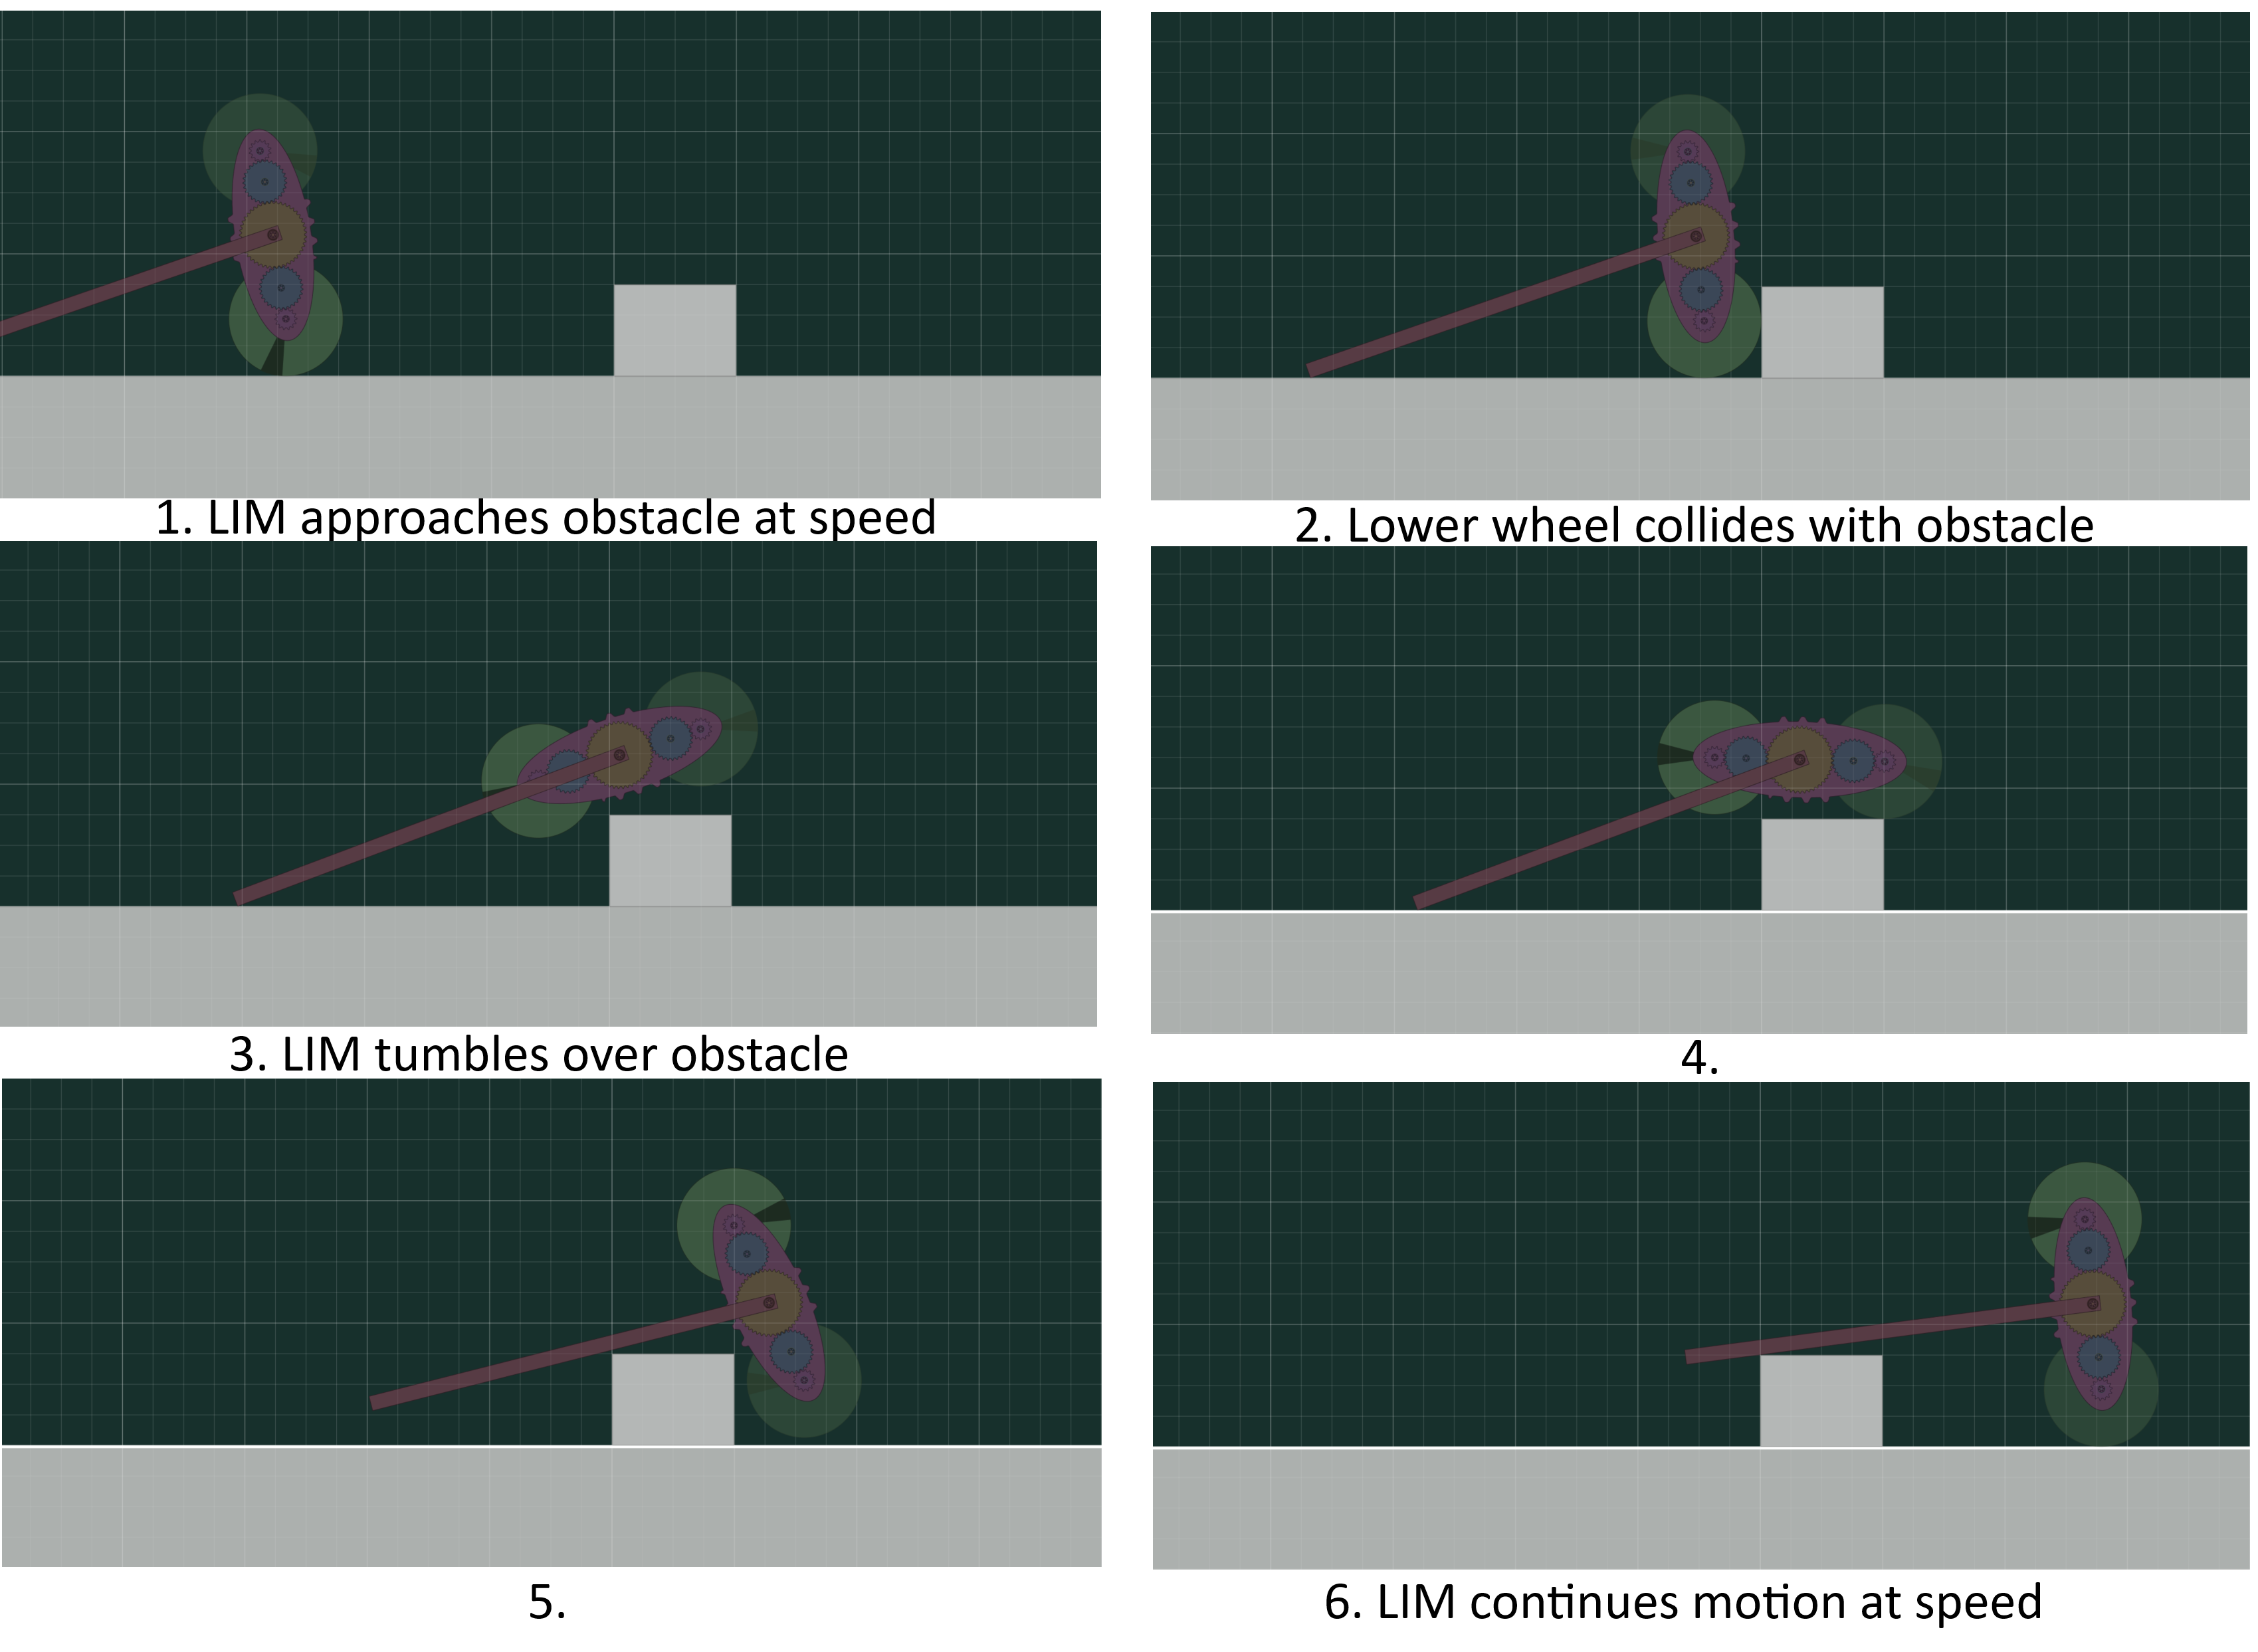
\includegraphics[width=1\textwidth]{algo-vert}
	\caption{Algodoo LIM system approaching obstacle vertically}
	\label{algo-vert}
\end{figure}

Another observation made was that if the LIM rolls at speed into the obstacle, it will have to absorb all the energy of the impact. None of the translational kinetic energy of the robot is transformed into rotational kinetic energy of the LIM for flipping. This results in quite an inefficient system. One option to mitigate this would be to implement a control system that solves the inverted pendulum problem in order to stand the LIMs upright on one wheel during normal operation. When the lower wheel encounters an obstacle while rolling, the LIM will readily flip over it without having to stop. The LIM could then switch to horizontal rolling when the robot needs a lower profile to enter a void. This solution would only be effective if a robust control system can be developed. These approaches are shown in Figures \ref{algo-hori} and \ref{algo-vert}.
\chapter{Maths Model}

\section{Overview and objectives}

This project develops a system of equations to analytically model the climbing motion of the device, which will be referred to as the, "Maths Model" henceforth. The intention behind this model is to allow designers to input parameters such as gear ratio, mass, wheel size, tail length, and motor torque, then determine whether the specified device will be able to climb steps. The equations can also reversed to solve for specific parameters, such as the motor torque required to lift a device with certain properties. The maths model is developed using the MATLAB symbolic toolbox.\\

\section{Definition of motions}

As a LIMed device climbs, the tail and wheels come into contact with different surfaces on the stairs and ground, which changes how the device moves. The overall climbing motion is broken down into sequential stages which are modelled individually. These stages are defined as follows:\\
\subsection*{Stage 0: Rolling}

When the LIMed device does is on a flat plane with no obstacle, it simply rolls forward. If the motor torque is high enough, the LIMs will flip even without an obstacle. However, DC motors lose torque as they gain speed, so the rolling motion prevents the motors from producing enough torque to flip the LIMs.\\

\subsection*{Stage 1: Lifting}
When the front wheel of the LIM comes into contact with the first step, it is blocked by a step and fixed in place. The tail pushes against the ground and the LIM starts rotating up the step. This motion ends when the LIM is vertical.
\\
\subsection*{Stage 2: Flipping}

Once the LIM is vertical, the bottom wheel starts to roll backwards as the top wheel falls forward onto the step. The distance that the bottom wheel rolls depends on the speed of the LIM and the height of the step. If the frame of the LIM hits the edge of the step, the device may slip backwards until the top wheel makes contact with the step. This motion ends when the top wheel is on the step.\\

\subsection*{Stage 3: Climbing}

The front wheel rests on the step while the back wheel is on the ground. The tail pushes against the ground and the back wheel lifts while the front wheel simultaneously rolls forward on the step. This motion ends when the front wheel reaches the next step.\\

Stages 1 to 3 will repeat until the tail leaves the ground. After this point the tail will push against the edge of the previous steps. 

\subsection*{Stage 4: Lifting from step}

Similar to Stage 1, but the tail pushes against the edge of a the previous step, which now applies a force pulling the device backwards. Assuming friction on the wheel is sufficient, the LIM starts rotating up the step. This motion ends when the LIM is vertical.

\subsection*{Stage 5: Flipping from step}

Similar to Stage 2, but the tail pushes against the edge of a the previous step, which now applies a force pulling the device backwards. This motion ends when the top wheel is on the step.\\

\subsection*{Stage 6: Climbing from step}

Similar to Stage 3, but the tail pushes against the edge of a the previous step, which now applies a force pulling the device backwards. The back wheel lifts while the front wheel rolls forward on the step. This motion ends when the front wheel reaches the next step; however, due to the tail force pulling the device backwards, the back wheel will continue to lift past the horizontal while front wheel rolls forward.\\


\section{Core equations and assumptions}

The maths model is consists of a system of equations that are solved simultaneously. These equations are derived from the free body diagrams of each component, and only consider movement in two dimensions. The components in question are the LIM frame, the sun gear, the idler gears, and the planet gears including the shaft and the wheels, and the body of the device. These components make contact with the surroundings and the other components, which exert equal and opposite forces on each other. As the maths model only considers movement in two dimensions, the LIMs are assumed to move synchronously. To simplify the equations, only one LIM is modelled, and its mass and moment of inertia is doubled.\\

Consider the device climbing a step as visualised in Figure \ref{Component-names}. Each component is assigned a number, where the LIM frame is 1, the sun gear is 2, the idler gears are 3 and 4, the planet gears, including the wheels, are 5 and 6, and the body of the device, including the tail, is 7.
\begin{figure}[h]
	\centering
	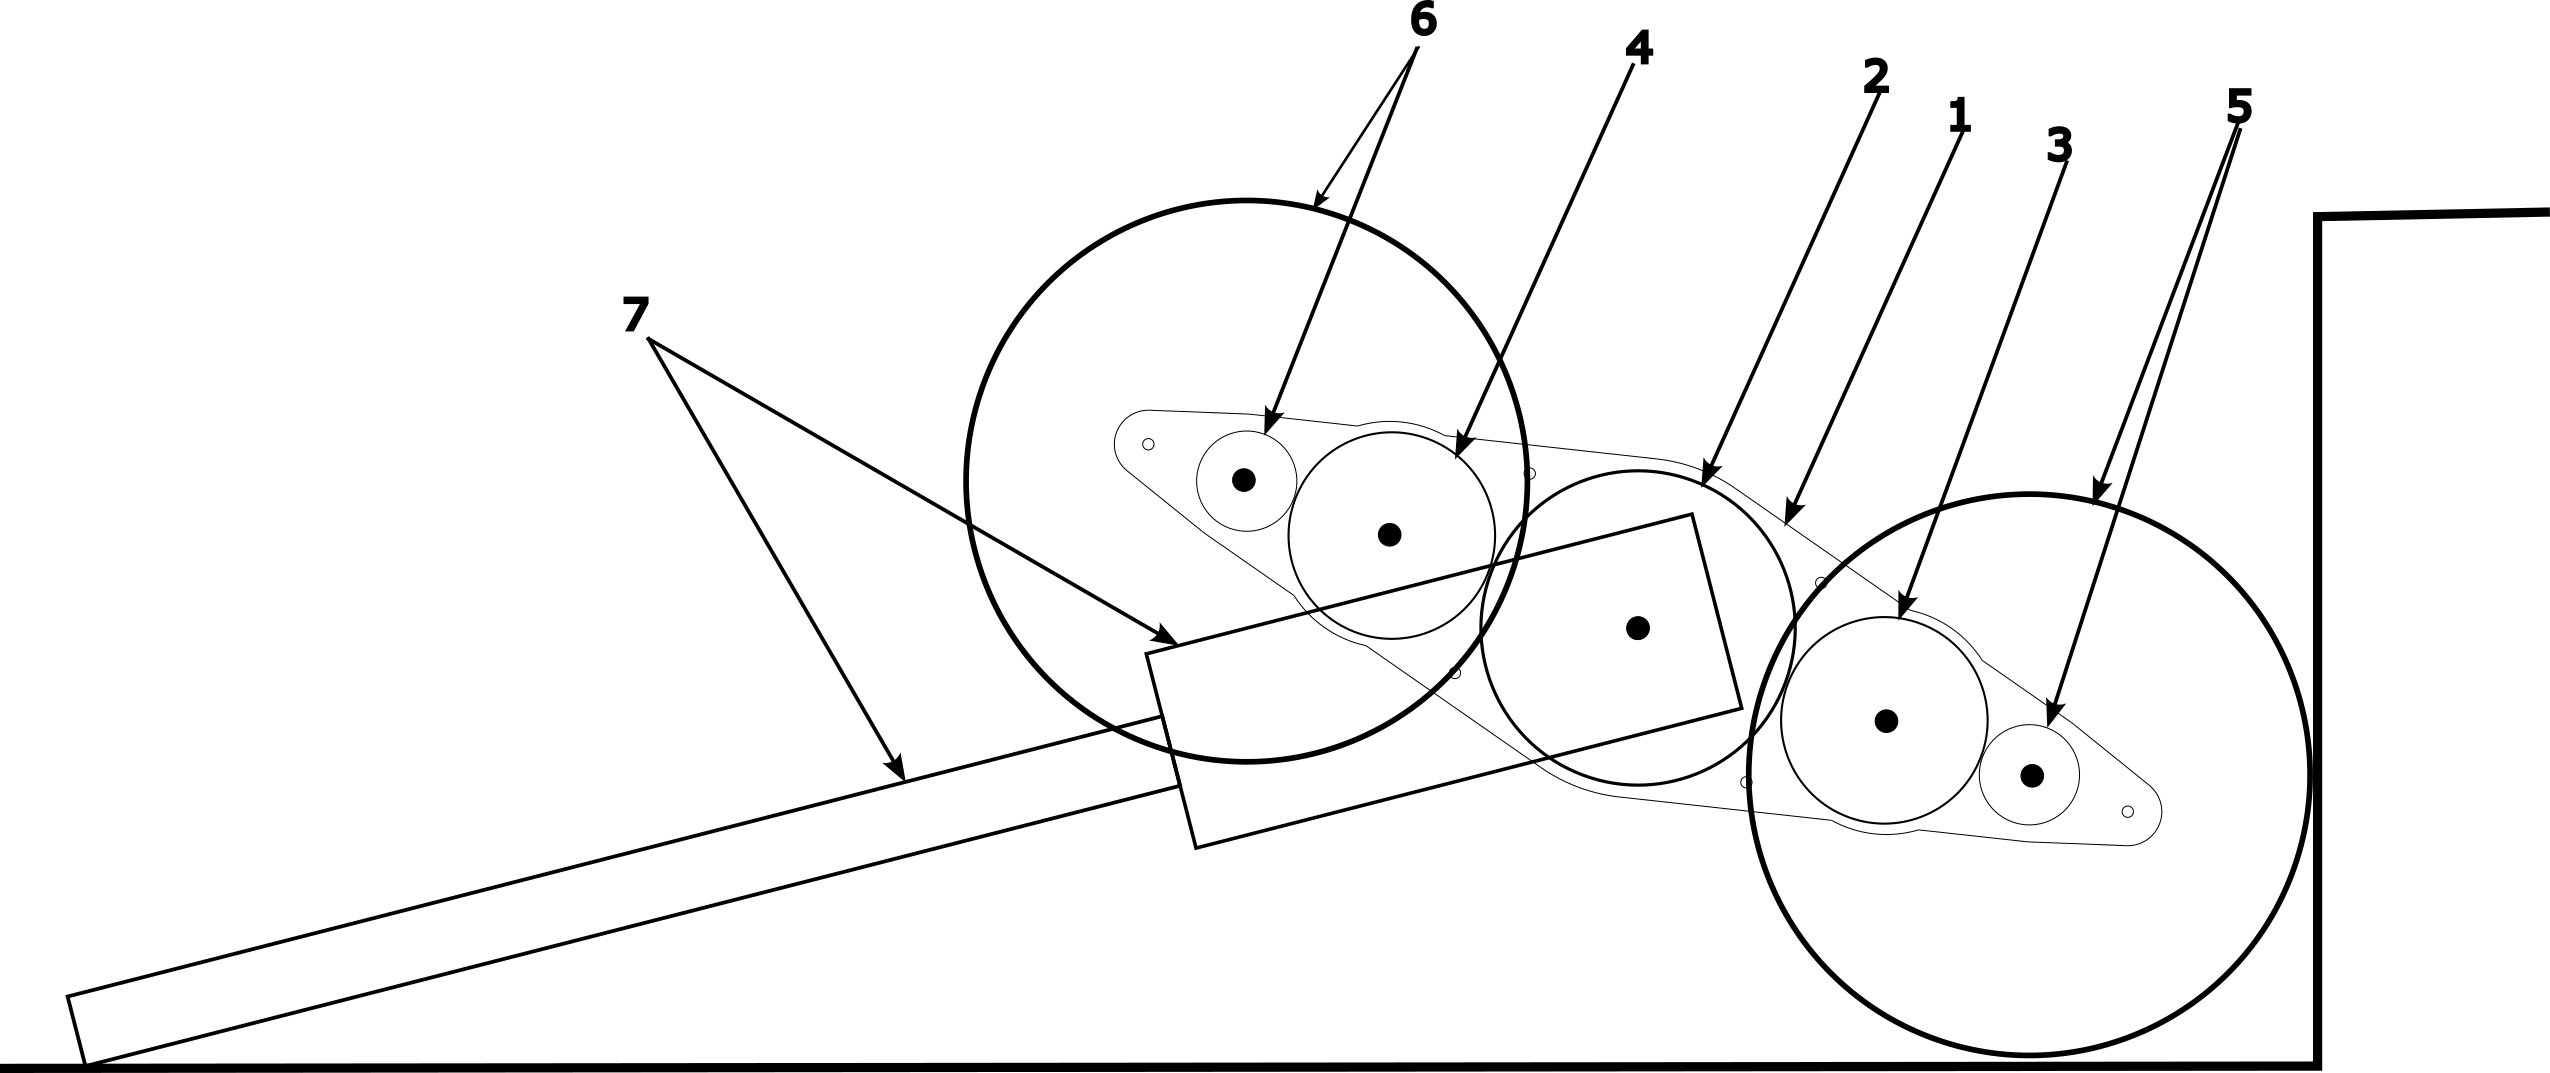
\includegraphics[width=0.8\textwidth]{FBDs/Naming components.png}
	\caption{Free body diagram of the LIM frame (component 1)}
	\label{Component-names}
\end{figure}
Powering the motor causes a torque between the body of the device and the SUN gear. The components of the device that make contact with the environment, namely the front wheel and the tail, will be subject to external reaction forces, which are dependent on the stage of motion. These forces and torques will propagate internally through the gears, causing a forward motion. The free body diagrams for each component are shown in Figures \ref{FBD-1} and \ref{FBD-2}.\\
\begin{figure}[h]
	\centering
	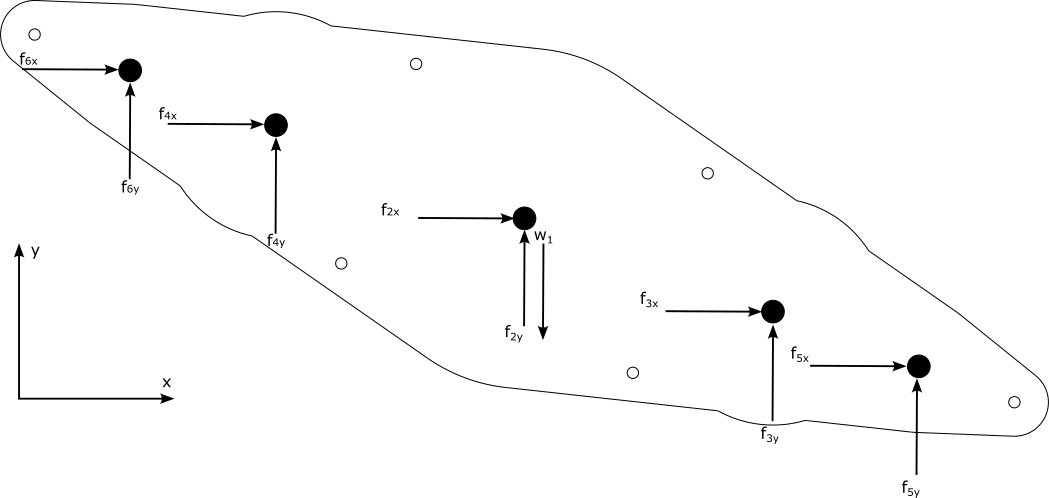
\includegraphics[width=1\textwidth]{FBDs/FBD-1.png}
	\caption{Free body diagram of the LIM frame (component 1)}
	\label{FBD-1}
\end{figure}
\begin{figure}[!h]
	\centering
	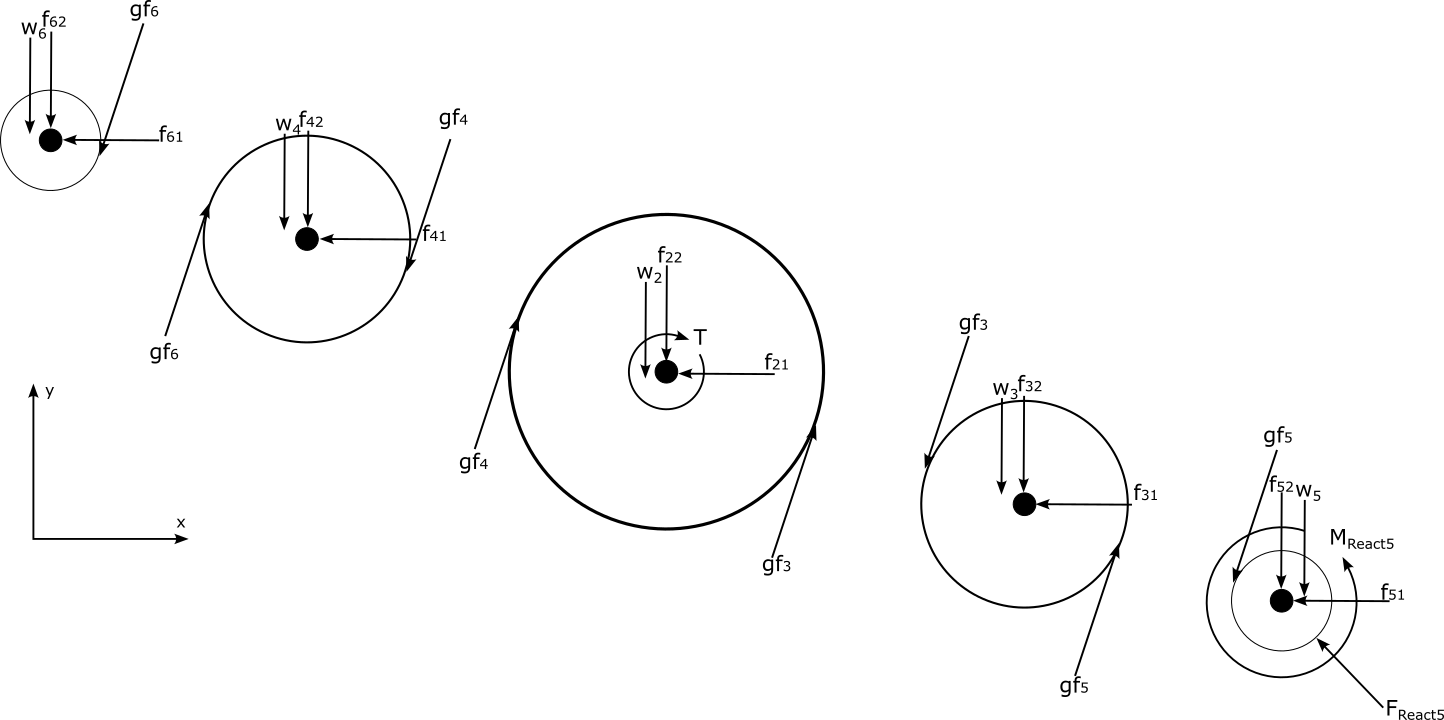
\includegraphics[width=1\textwidth]{FBDs/FBD-2.png}
	\caption{Free body diagram of the gears (components 2-5)}
	\label{FBD-2}
\end{figure}

Each component exerts a force on connected components, which exert an equal and opposite force back.
For example, the the sum of forces equations for the sun gear are,\\
\begin{equation}
	m_2\vec{a_2} == \vec{w_2}-\vec{f_2}+\vec{\mathrm{gf}_3}+\vec{\mathrm{gf}_4}
\end{equation}
Where $m_x$ refers to the mass of component $x$, $\vec{a_x}$ is the acceleration vector of component $x$, $\vec{w_x}$ is the weight vector of component $x$, $\vec{f_x}$ is the force vector that component $x$ applies to component 1,  and $\vec{\mathrm{gf}_3}$ and $\vec{\mathrm{gf}_4}$ are the force vectors that components 3 and 4 respectively apply to component 2 through the gears.
This can be expanded to,
\begin{equation}
	m_2
	\begin{bmatrix}
		a_{21}\\
		a_{22}\\
		a_{23}\\
	\end{bmatrix}
	=
	\begin{bmatrix}
		w_{21}-f_{21}+\mathrm{gf}_{31}+\mathrm{gf}_{41}\\
		w_{22}-f_{22}+\mathrm{gf}_{32}+\mathrm{gf}_{42}\\
		w_{23}-f_{23}+\mathrm{gf}_{33}+\mathrm{gf}_{43}\\
	\end{bmatrix}
\end{equation}
where vector positions 1, 2, and 3 denote the x, y, and z dimensions respectively. This equation can be further simplified by restraining movement to the x and y dimensions, and substituting $\vec{w_2} = \begin{bmatrix} 0 & m_2g & 0 \end{bmatrix}'$,
\begin{equation}
	m_2
	\begin{bmatrix}
		a_{21}\\
		a_{22}\\
	\end{bmatrix}
	=
	\begin{bmatrix}
		-f_{21}+\mathrm{gf}_{31}+\mathrm{gf}_{41}\\
		m_2g-f_{22}+\mathrm{gf}_{32}+\mathrm{gf}_{42}\\
	\end{bmatrix}
\end{equation}
Similarly, the sum of moments equation for the sun gear is derived
\begin{equation}
	I_2\ddot{\theta_2} == T - r_2|\vec{\mathrm{gf}_3}| + r_2|\vec{\mathrm{gf}_3}|
\end{equation}
where $I_2$ is the moment of inertia of component 2, $\theta_2$ is the angle of component 2, $T$ is the moment exerted by the motor on component 2, and $r_2$ is the radius of component 2. Note that in this project, all angles and moments are given in the clockwise direction.
\\
The full list of equations can be found in appendix ??? and in the matlab code.



\section{Boundary conditions}
Depending on the stage of the climbing, components of the device will come into contact with different parts of the steps and at different angles. To model climbing in each stage, a set of equations defining the contact is given for each stage.\\
\subsection*{Stage 1: Lifting}
The front wheel, referred to as component 5, is locked in place by the reaction forces from the step, this leads to the condition,
\begin{subequations}
	\label{wheel1locked}
	\begin{align}
		\vec{a_5} &= \vec{0}\\
		\vec{v_5} &= \vec{0}\\
		\dot{\theta}_5 &= 0\\
		\ddot{\theta}_5 &= 0
	\end{align}
\end{subequations}
where $\vec{v_x}$ refers to the velocity of component $x$. \\
The front wheel must be placed into a two dimensional coordinate system. In stage 1, the front wheel can be on the ground or on one of the steps, so long as the tail can reach the ground, and the front wheel will always be pressed against the edge of the next step. Placing the origin at the start of the steps, the position of the wheel can be defined as,
\begin{equation}
	\vec{s_5}
	=
	\begin{bmatrix}
		\mathrm{StepWidth}\cdot N-r_w\\
		\mathrm{StepHeight}\cdot N+r_w\\
		0
	\end{bmatrix}
\end{equation}
where $\vec{s_5}$ is the position vector of the centre of the front wheel, $N$ is the number of the step on which the wheel is placed, with $N = 0$ placing the step on the ground, and $r_w$ is the radius of the wheel.\\
The end of the tail pushes against the ground, which leads to the following conditions,
\begin{subequations}
	\label{tailonground}
	\begin{align}
		s_{7end2} &= 0\\
		F_{react71} &=  -\mu_{tail}F_{react72}\\
		-\ddot{\theta_7} &= \frac{(|\vec{l_7}|^2 - l_{72}^2)a_{12} + l_{72}v_{12}^2}{|\vec{l_7}|^3 (1 - \frac{l_{72}^2}{|\vec{l_7}|^2})^{3/2}} \label{tailongroundkinematics}
	\end{align}
\end{subequations}
where $s_{7end2}$ is the y position of the endpoint of the tail, $F_{react71}$ and $F_{react72}$ are the reaction forces exerted onto the tail by the ground in the x and y dimensions respectively, $\mu_{tail}$ is the coefficient of friction between the tail and the ground, $\vec{l_7}$ is the position of the end of the tail relative to the motor axle, and $l_{72}$ is the component of $\vec{l_7}$ in the y dimension. \\
Equation \ref{tailongroundkinematics} is derived from,

\begin{subequations}
	\begin{align}
		-\theta_7(t) &= \arcsin{\frac{l_{72}(t)}{|\vec{l_7}|}}\\
		\frac{d^2}{dt^2}-\theta_7(t) &= \frac{d^2}{dt^2}\arcsin{\frac{l_{72}(t)}{|\vec{l_7}|}}
	\end{align}
\end{subequations}
where $\theta_7$ and $l_{72}$ are treated as functions of time, $t$. This relation can be seen in figure ???. $v_{12}$ and $a_{12}$ refer to the velocity and acceleration of the motor axle in the y dimension, and are equivalent to $-\dot{l}_{72}$ and $-\ddot{l}_{72}$ respectively.\\ ??????? verify

\subsection*{Stage 2: Flipping}

Once the LIM is vertical, there is no longer a force pushing the bottom wheel forward into the step, instead it rolls backwards. This leads to a new condition,
\begin{subequations}
	\label{wheel1rolling}
	\begin{align}
		\vec{a_5} &= \begin{bmatrix}
			\ddot{\theta}_5 r_w \\
			0\\
			0
		\end{bmatrix}\\
		\vec{v_5} &= \begin{bmatrix}
			\dot{\theta}_5 r_w \\
			0\\
			0
		\end{bmatrix}\\
		s_{51} &= \theta_{5} r_w;\\
		M_{react5} &= - F_{react51} r_w;
	\end{align}
\end{subequations}
where $M_{react5}$ is the reaction moment on wheel 5 as a result of the reaction forces.
The tail is still on the ground, so will still be subject to Equations \ref{tailonground}.

\subsection*{Stage 3: Climbing}

In Stage 3, the front and back wheel have swapped. To simplify the movements, component 5 will always refer to the wheel that makes contact with the steps, and component 6 will refer to the wheel that does not. \\
The front wheel is rolling and the tail is on the ground, which are the same conditions as in Stage 2. As such, Stage 3 is subject to Equations \ref{wheel1rolling} and \ref{tailonground}.

\subsection*{Stage 4: Lifting with tail on step}
Stage 4 is similar to stage 1, except the tail is on the step. As such, this motion is subject to Equations \ref{wheel1locked} because the wheel is locked, and a set of new conditions because the tail is on the edge of the step,

\begin{subequations}
	\label{tailonstep}
	\begin{align}
		u_1 &= \mathrm{StepWidth}\cdot (N_2-1)- s_{11}\\
		u_2 &= \mathrm{StepHeight}\cdot N_2 - s_{12}\\
		\tan{(-\theta_7)} &= \frac{u_2}{u_1}\\
		\label{tailonstepposition}
		-\ddot{\theta_7} &= \frac{ u_1^2 (a_{11} u_2  - 2 v_{11} v_{12}) 
			+ u_2^2 (a_{11} u_2 + 2  v_{11}  v_{12}  )  
			-  a_{12} u_1^3 
			- u_1  u_2  (- 2  v_{11}^2 + 2 v_{12}^2 + a_{12} u_2  )}
		{(u_1^2 + u_2^2)^2}\\
		\label{tailonstepaccelleration}
		F_{react71}' &= -\mu_{tail} F_{react72}'\\
		\vec{F}_{react7} &= \begin{bmatrix}
			-\cos{(\theta_7)} & -\sin{(\theta_7)} & 0\\
			\sin{(\theta_7)} & -\cos{(\theta_7)} & 0\\
			0 & 0 & 1
		\end{bmatrix} \vec{F}_{react7}'
	\end{align}
\end{subequations}
where $N_2$ is the number of the step that the tail makes contact with, $u_1$ and $u_2$ are the displacement from the motor axis to the point of contact with the step. Equation \ref{tailonstepaccelleration} is the second derivative of \ref{tailonstepposition}. $\vec{F}_{react7}'$ is the vector of reaction forces in a rotated coordinate system such that $F_{react72}'$ is the normal force between the tail and the step.

\subsection*{Stage 5: Flipping from step}
Stage 5 is similar to stage 2, except the tail is on the step. As such, this motion is subject to Equations \ref{wheel1rolling} because the wheel is locked, and Equations \ref{tailonstep} because the tail is on the step.\\

\subsection*{Stage 6: Climbing from step}
Stage 6 is similar to stage 3, except the tail is on the step. As such, this motion is subject to Equations \ref{wheel1rolling} because the wheel is locked, and Equations \ref{tailonstep} because the tail is on the step.\\

\section{Solving technique}
The MATLAB symbolic toolbox comes with the solve() function, which can be used to solve sets of non-linear simultaneous equations. However, it struggles with this large set of equations that contain trigonometric functions, often stalling. This project develops a function that breaks down the set of equations into smaller, easier to solve sets, then substituting these solutions into the remaining equations. Figure ??? shows the flowchart for this function. \\
\\
The function loops through the equations until they have all been solved, or it cannot find any more solutions. First, it identifies any trivial equations that contain only one variable, such as $a = 1$, and solves them. This will also pick up equations with more than one solution, such as $\sin{a} = 1$; to resolve this, the solver will look for inequalities that contain the relevant variable, in this case $a$, and apply them to the solution. For example, if you were to provide the function with the set of equations:\\

\begin{subequations}
	\label{exampleinput}
	\begin{align}
		a &= 0.5 \label{example1a}\\
		\sin{(b)} &= a\\
		b &>= \frac{\pi}{2}\\
		b &<= \pi
	\end{align}
\end{subequations}
The first loop would identify Equation \ref{example1a} as it only has one variable. It wouldn't find any inequalities that describe the variable $a$ so it would simply send the equation $a = 0.5$ to MATLAB's solve() function. It then records the solution and substitutes it into the remaining equations, 
\begin{subequations}
	\label{example2}
	\begin{align}
		\sin{(b)} &= 0.5 \label{example2a}\\
		b &>= \frac{\pi}{2}\label{example2b}\\
		b &<= \pi\label{example2c}
	\end{align}
\end{subequations}
The second loop identifies Equation \ref{example2a} as it only has one variable. It looks for inequalities that describe $b$ and finds Inequalities \ref{example2b} and \ref{example2c}. It then sends all three to MATLAB's solve() function, which returns the solution for $b$.
The function then outputs a structure with the fields,
\begin{subequations}
	\begin{align}
		\mathrm{solution.a} &= 0.5\\
		\mathrm{solution.b} &= \frac{5\pi}{6}
	\end{align}
\end{subequations}

Once the function can no longer find trivial solutions, it looks for sets of equations that contain the exact same variables, such as equations of the form,
\begin{subequations}
	\begin{align}
		a -2b &= 0\\
		b -a +2 &= 0 
	\end{align}
\end{subequations}
and sends them to be solved. For this to work, there must be at least as many equations as there are variables in the set. This function will also identify and delete duplicate equations.\\
Once the function can no longer find sets of equations that use the exact same variables, it will attempt to find sets of equations that fully describe a set of variables, such as,
\begin{subequations}
	\begin{align}
		a -3b &= 0\\
		b -c +2&= 0\\
		a -2c &= 0
	\end{align}
\end{subequations}
Finally, if it can't find any fully defined sets up to a certain size, it will attempt to solve the complete set of remaining equation using the solve() function. If the function is unable to solve all the equations, it will return a structure containing the solutions it has found, and a vector containing the remaining equations.


\section{Required torque}
When designing a LIM robot, it is essential to size the motor and gearbox to be able to provide enough torque to lift the LIMs. To do this, one must first determine which stage of motion requires the most torque. To find the minimum torque required to cause forward movement, we solve for the torque that results in an overall acceleration of 0 when the velocity is also 0, essentially adding the conditions:
\begin{subequations}
	\label{condition-static}
	\begin{align}
		\vec{a} &= \vec{0}\\
		\vec{v} &= \vec{0}\\
		\ddot{\theta_1} &= 0\\
		\dot{\theta_1} &= 0\\
	\end{align}
\end{subequations}
which simplifies the dynamic equations into static equations.\\
The set of equations is then solved for a range of positions in each stage.
\subsection*{Stage 1: Lifting}
During the lifting motion, the angle of the LIMs, $\theta_1$, increases from 0° when the LIM is horizontal to 90° when the LIM is vertical. Figure \ref{torque-angle-relation-stage1} shows that the required torque is highest when the LIM is horizontal, which in this particular device is 1.014 Nm, or 0.507 Nm per motor.
\begin{figure}[h]
	\centering
	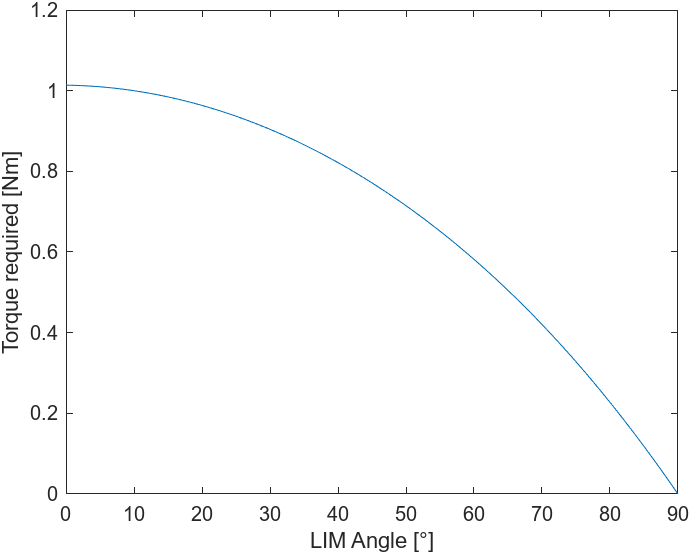
\includegraphics[width=0.8\textwidth]{plots/torque-angle-relation-stage1}
	\caption{Relationship between LIM angle and required torque for Stage 1 motion}
	\label{torque-angle-relation-stage1}
\end{figure}
\subsection*{Stage 2: Flipping}
During the flipping motion, the device does not need any torque to move. Even without a torque input, it will simply fall onto the next step.

\subsection*{Stage 3: Climbing}
During the climbing motion, the LIMs lift from the starting position, in this case -42.5° to the horizontal 0°. In addition, the front wheel can roll forward, instead of solving for the torque that results in an overall forward acceleration, we solve for the torque that causes a positive vertical acceleration in the back wheel. Instead of Equations \ref{condition-static}, we have:
\begin{subequations}
	\label{condition-climbing}
	\begin{align}
		a_{62} &= 0\\
		\vec{v} &= \vec{0}\\
		\dot{\theta_1} &= 0\\
	\end{align}
\end{subequations}
Figure \ref{torque-angle-relation-stage3} shows that the required torque increases as the LIM lifts, until the maximum of 0.970 Nm, or 0.485 Nm per motor when the LIM is horizontal.
\begin{figure}[h]
	\centering
	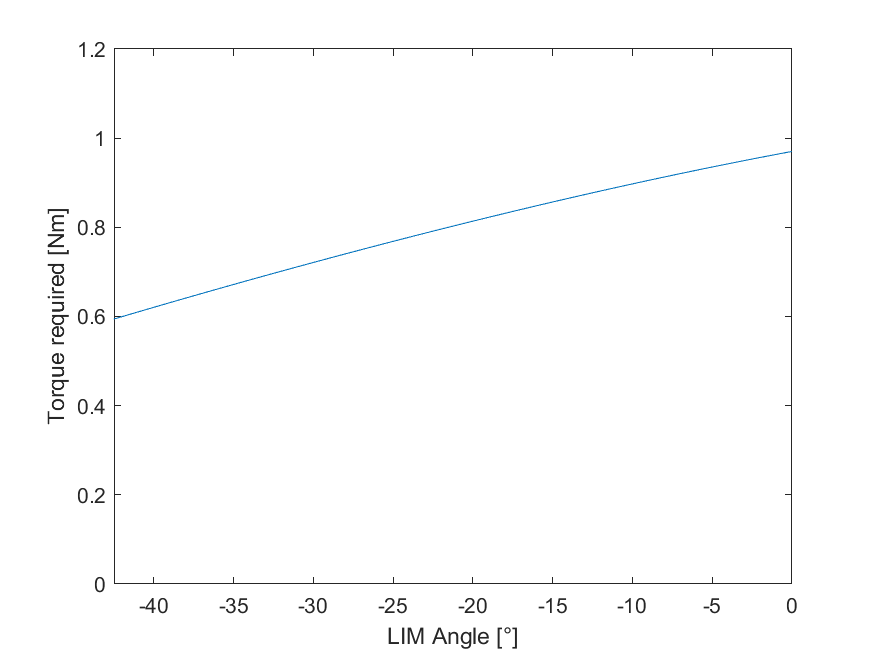
\includegraphics[width=0.8\textwidth]{plots/torque-angle-relation-stage3}
	\caption{Relationship between LIM angle and required torque for Stage 3 motion}
	\label{torque-angle-relation-stage3}
\end{figure}

\subsection*{Stage 4: Lifting from step}
Similar to Stage 1, $\theta_1$ increases from 0° when the LIM is horizontal to 90° when the LIM is vertical. Figure \ref{torque-angle-relation-stage4} shows that for this device, the required torque is highest when the LIM is at 26.4°, which gives a required torque of 1.295 Nm, or 0.647 Nm per motor.
\begin{figure}[h]
	\centering
	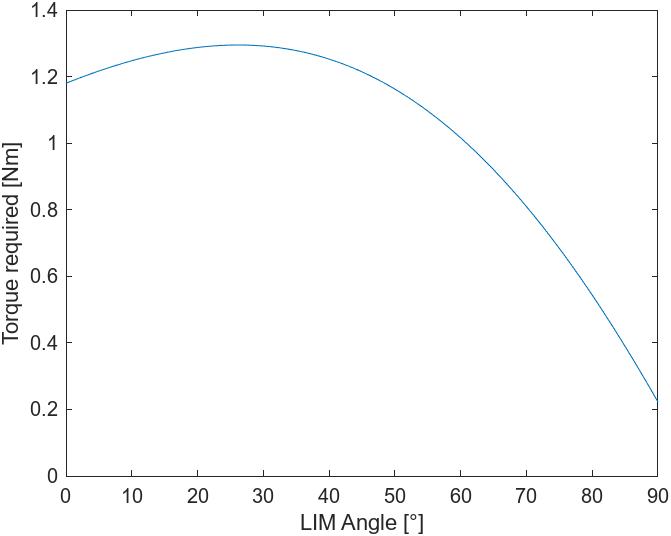
\includegraphics[width=0.8\textwidth]{plots/torque-angle-relation-stage4}
	\caption{Relationship between LIM angle and required torque for Stage 4 motion}
	\label{torque-angle-relation-stage4}
\end{figure}


\subsection*{Stage 5: Flipping from step}
During the flipping motion, the device does not need any torque to move. Even without a torque input, it will simply fall onto the next step.

\subsection*{Stage 6: Climbing from step}
Similar to Stage 3, $\theta_1$ increases from -42.5° to 0°, and Equations \ref{condition-climbing} are used instead of Equations \ref{condition-static}. Figure \ref{torque-angle-relation-stage6} shows that for this device, the required torque is highest when the LIM is horizontal, which gives a required torque of 1.228 Nm, or 0.614 Nm per motor.
\begin{figure}[h]
	\centering
	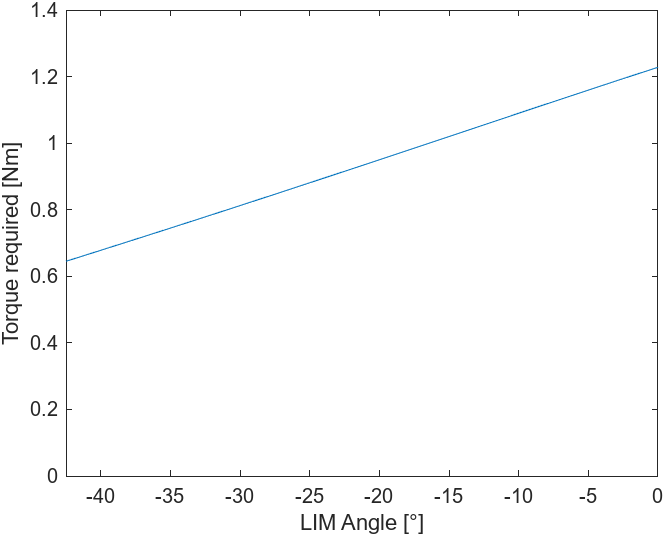
\includegraphics[width=0.8\textwidth]{plots/torque-angle-relation-stage6}
	\caption{Relationship between LIM angle and required torque for Stage 6 motion}
	\label{torque-angle-relation-stage6}
\end{figure}
These plots show that the highest required torques will be in Stages 4 and 6, and that the particular device modelled requires an output torque of at least 0.647 Nm on each motor.

\subsection{Sizing components to reduce torque requirement}
So far this section has only modelled a device with fixed parameters, such as gear ratio, wheel size, mass, and tail length, however a designer may be interested in varying these parameters. The model can be used to inform the design process by showing the effect that changing certain parameters has on the required torque. For example, Figure ??? shows how changing the gear ratio affects the torque required.


\section{Required coefficient of friction}

When the device climbs steps, it is possible that the front wheel, component 5, will slip. Applying the coulomb approximation of friction to the model, Slipping will occur when $|F_{51}| > \mu_5 F_{52}$, where $\mu_5$ is the coefficient of friction between the wheel and the step. This coefficient can be increased by using certain materials, such as rubber, for the contact surface of the wheels. However, the coefficient of friction is also dependent on the material of the step itself, which a designer would not have control over. For this reason, designers may want to modify the design to reduce the required coefficient of friction.\\
Similar to the required torque, the coefficient of friction required to prevent slipping can also be calculated across the motion, and the highest value is in Stage 4. The parameters can be 

\chapter{Design requirements}

The objective of the design phase is to design a LIMed platform that can be used to validate the mathematical model. The requirements for this design are documented in this section.

\section{Stakeholder requirements}

This project is done at the request of Justin Pead, who supervised previous LIM projects at UCT. For the purposes of this section, this project's supervisor, Mr. Wayne Swart, acts as an intermediary between the stakeholder and the designer. 


\begin{table}[h]
	\caption{Stakeholder requirements.}
	\footnotesize
	\begin{tabular}{ | p{3em} | p{6em} | p{23em} | p{5em} |} 
		\hline
		Number& Stakeholder & Description & Priority \\ 
		\hline
		SR1 & Justin Pead & The device must be able to climb stairs & High\\
		\hline
		SR2 & Justin Pead & The device must roll on its wheels when it is not obstructed, and climb over obstacles when it is obstructed. & High\\
		\hline
		SR3 & Justin Pead & The device must use LIMs for locomotion & Must-have\\
		\hline
		SR4 & Justin Pead & The device should be described by the model & Must have\\
		\hline
		SR5 & Justin Pead & The device should be relevant to USAR applications & High\\
		\hline
		SR6 & Wayne Swart & The design and construction of the device must demonstrate the relevant graduate attributes & Must have\\
		\hline
		SR7 & Wayne Swart & The budget for the project is R5000 & Must have\\
		\hline
	\end{tabular}
\end{table}
\newpage

\section{Engineering requirements}

In this section, the stakeholder requirements (SRs) are expressed as functional requirements (FRs) and performance requirements (PRs). FRs describe the actions that the system must perform, while PRs are measures of how well the system performs the functions.

\begin{table}[h]
	\caption{Functional requirements.}
	\footnotesize
	\begin{tabular}{ | p{4em} | p{28em} | p{6em} |} 
		\hline
		Number & Description & Relevant Stakeholder Requirement\\
		\hline
		FR1 & Climb obstacles & SR1, SR2\\
		\hline
		FR2 & Roll & SR2\\
		\hline
		FR3 & Accept user control & SR5\\
		\hline
	\end{tabular}
\end{table}

\begin{table}[h]
	\caption{Performance requirements.}
	\footnotesize
	\begin{tabular}{ 	| p{4em} 	| p{13em} 		| p{4em} 	| p{4em} 	| p{2em} 	| p{6em} |} 
		\hline
						Number & 	Description & 	Target & 	Range & 	Unit & 		Relevant Stakeholder Requirement\\
		\hline
		PR1 & Height of obstacles that can be climbed & Maximise & 200+ \tablefootnote{Maximum step rise specified by the SANS10400 building regulation \citep{SANS}} & mm &  SR1, SR2\\
		\hline
		PR2 & Climbing success rate & Maximise & 90 - 100 & \% &  SR1, SR2\\
		\hline
		PR3 & Top speed & Maximise & 1+ & $m/s$ &  SR2\\
		\hline
		PR4 & Acceleration & Maximise & 1+ & $m/s^2$ &  SR2\\
		\hline
		PR5 & Height Clearance & Minimise & 50 - 300 & $mm$ &  SR5\\
		\hline
		PR6 & Cost & Minimise & 0 - 5000 & ZAR &  SR6\\
		\hline
	\end{tabular}
\end{table}


\chapter{Design}

In order to validate the model, a device must be designed, built and tested. 

\section{Selection of design parameters}
There are many parameters to consider when designing LIMs, such as gear ratios, lengths, and wheel size. Optimising the design is beyond the scope of this project, but the device does need to work to the extent that it can be used to validate the model. Initially, this project intended to use the early versions of the model to inform the design process. However, as the model was not yet validated, significantly changing key parameters could easily result in a device that is unable to climb stairs at all. Previous projects were able to show inconsistent success. Of the previous projects, Powrie's design was the latest and most informed, and is used as a starting point for this project. Powrie's report specifies the dimensions and gear ratios for the LIMs used in this project.\\

\section{Body design}
The body of the device is the central part that contains the motors and any peripheral devices.
Powrie's design for the body includes a camera, batteries, and extra gearing to increase the torque of his motor. These components are superfluous for the objectives of this project, and are not included in the design. Additionally, the body in Powrie's design protrudes forward significantly beyond the axle of the LIMs. This is done to allow for gearing of the axial motors used in the design, but previous students have found that this protrusion causes the body to collide with the step when climbing, which can result in failure to climb the step. This project uses DC motors with worm gearbox outputs, allowing the motor to be placed at a right angle to the axis. This eliminates the need for significant forward protrusion or additional gearing, and simplifies the construction process. Figures \ref{fig:Powrie-internals} and \ref{fig:internals} shows the body of Powrie's design and this project's design respectively.
\begin{figure}
	\centering
	\begin{subfigure}{.5\textwidth}
		\centering
		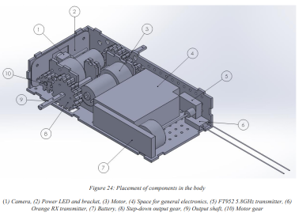
\includegraphics[width=.9\linewidth]{Powrie-internals}
		\caption{Powrie's design of the body.}
		\label{fig:Powrie-internals}
	\end{subfigure}%
	\begin{subfigure}{.5\textwidth}
		\centering
		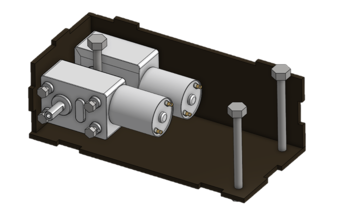
\includegraphics[width=.9\linewidth]{internals}
		\caption{This project's design of the body.}
		\label{fig:internals}
	\end{subfigure}
	\caption{Body design comparison.}
	\label{fig:bodies}
\end{figure}

\section{Motor selection}
Brushed DC motors often include a gearbox to increase the torque of the output at the cost of speed. For this design, the output shaft must be at a right angle to the motor, which is typically done with a worm gearbox. The most readily available motors that meet these requirements are the JGY-370 12V DC worm gear motors, which come with a range of gear ratios. Initially, the 40 RPM model was selected as it provides similar torque to the EGB-380S with added gearing that Powrie used, however initial tests indicated that additional torque was needed for consistent climbing, so the 6 RPM model was used instead.\\
Additionally, these motors have a self-locking gearbox, which improves the controllability of the device, as shutting off the motors will cause the gearbox to lock and the device to stop moving, rather than allowing the device to fall backwards down the steps.

\section{Control circuits and code}
In order to validate the model, the torque of the motors must be variable and reversible. This project uses a L298n H-bridge controlled by an STM32-F303RE Nucleo board to drive the motors. Two potentiometer sliders are used to control the torque of the two motors independently. The sliders are set up as voltage dividers and connected to the ADC channels of the STM32 microcontroller. The microcontroller sends a direction and PWM signal for each motor to the L298n H-bridge, which controls the motor using PWM. The circuit diagram for this set-up is shown in Figure \ref{fig:circuit-diagram}.\\

\begin{figure}[!h]
	\centering
	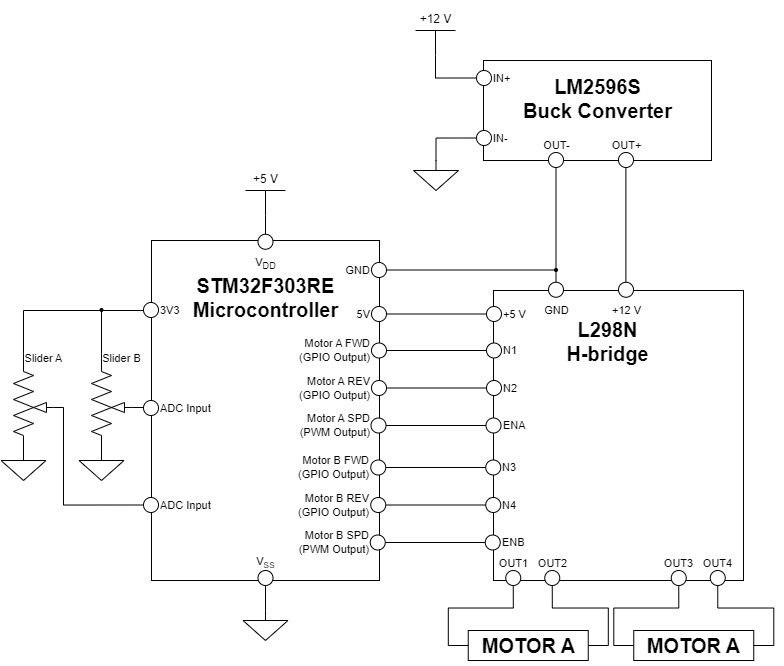
\includegraphics[width=0.8\textwidth]{circuit-diagram}
	\caption{Control system circuit diagram.}
	\label{fig:circuit-diagram}
\end{figure}

The microcontroller is programmed to power off the motors when the sliders are centred, move the motors forward when the sliders are pushed forward, and move the motors in reverse when the sliders are pulled back. The PWM duty cycle is scaled such that when the ADC values are in the centre 20\% of their range, the PWM duty cycle is set to 0\%. When the ADC values are within the top or bottom 5\% of their range, the duty cycle is 100\%. The flow diagram for this code is shown in Figure \ref{fig:controller-flowchart}.

\begin{figure}[!h]
	\centering
	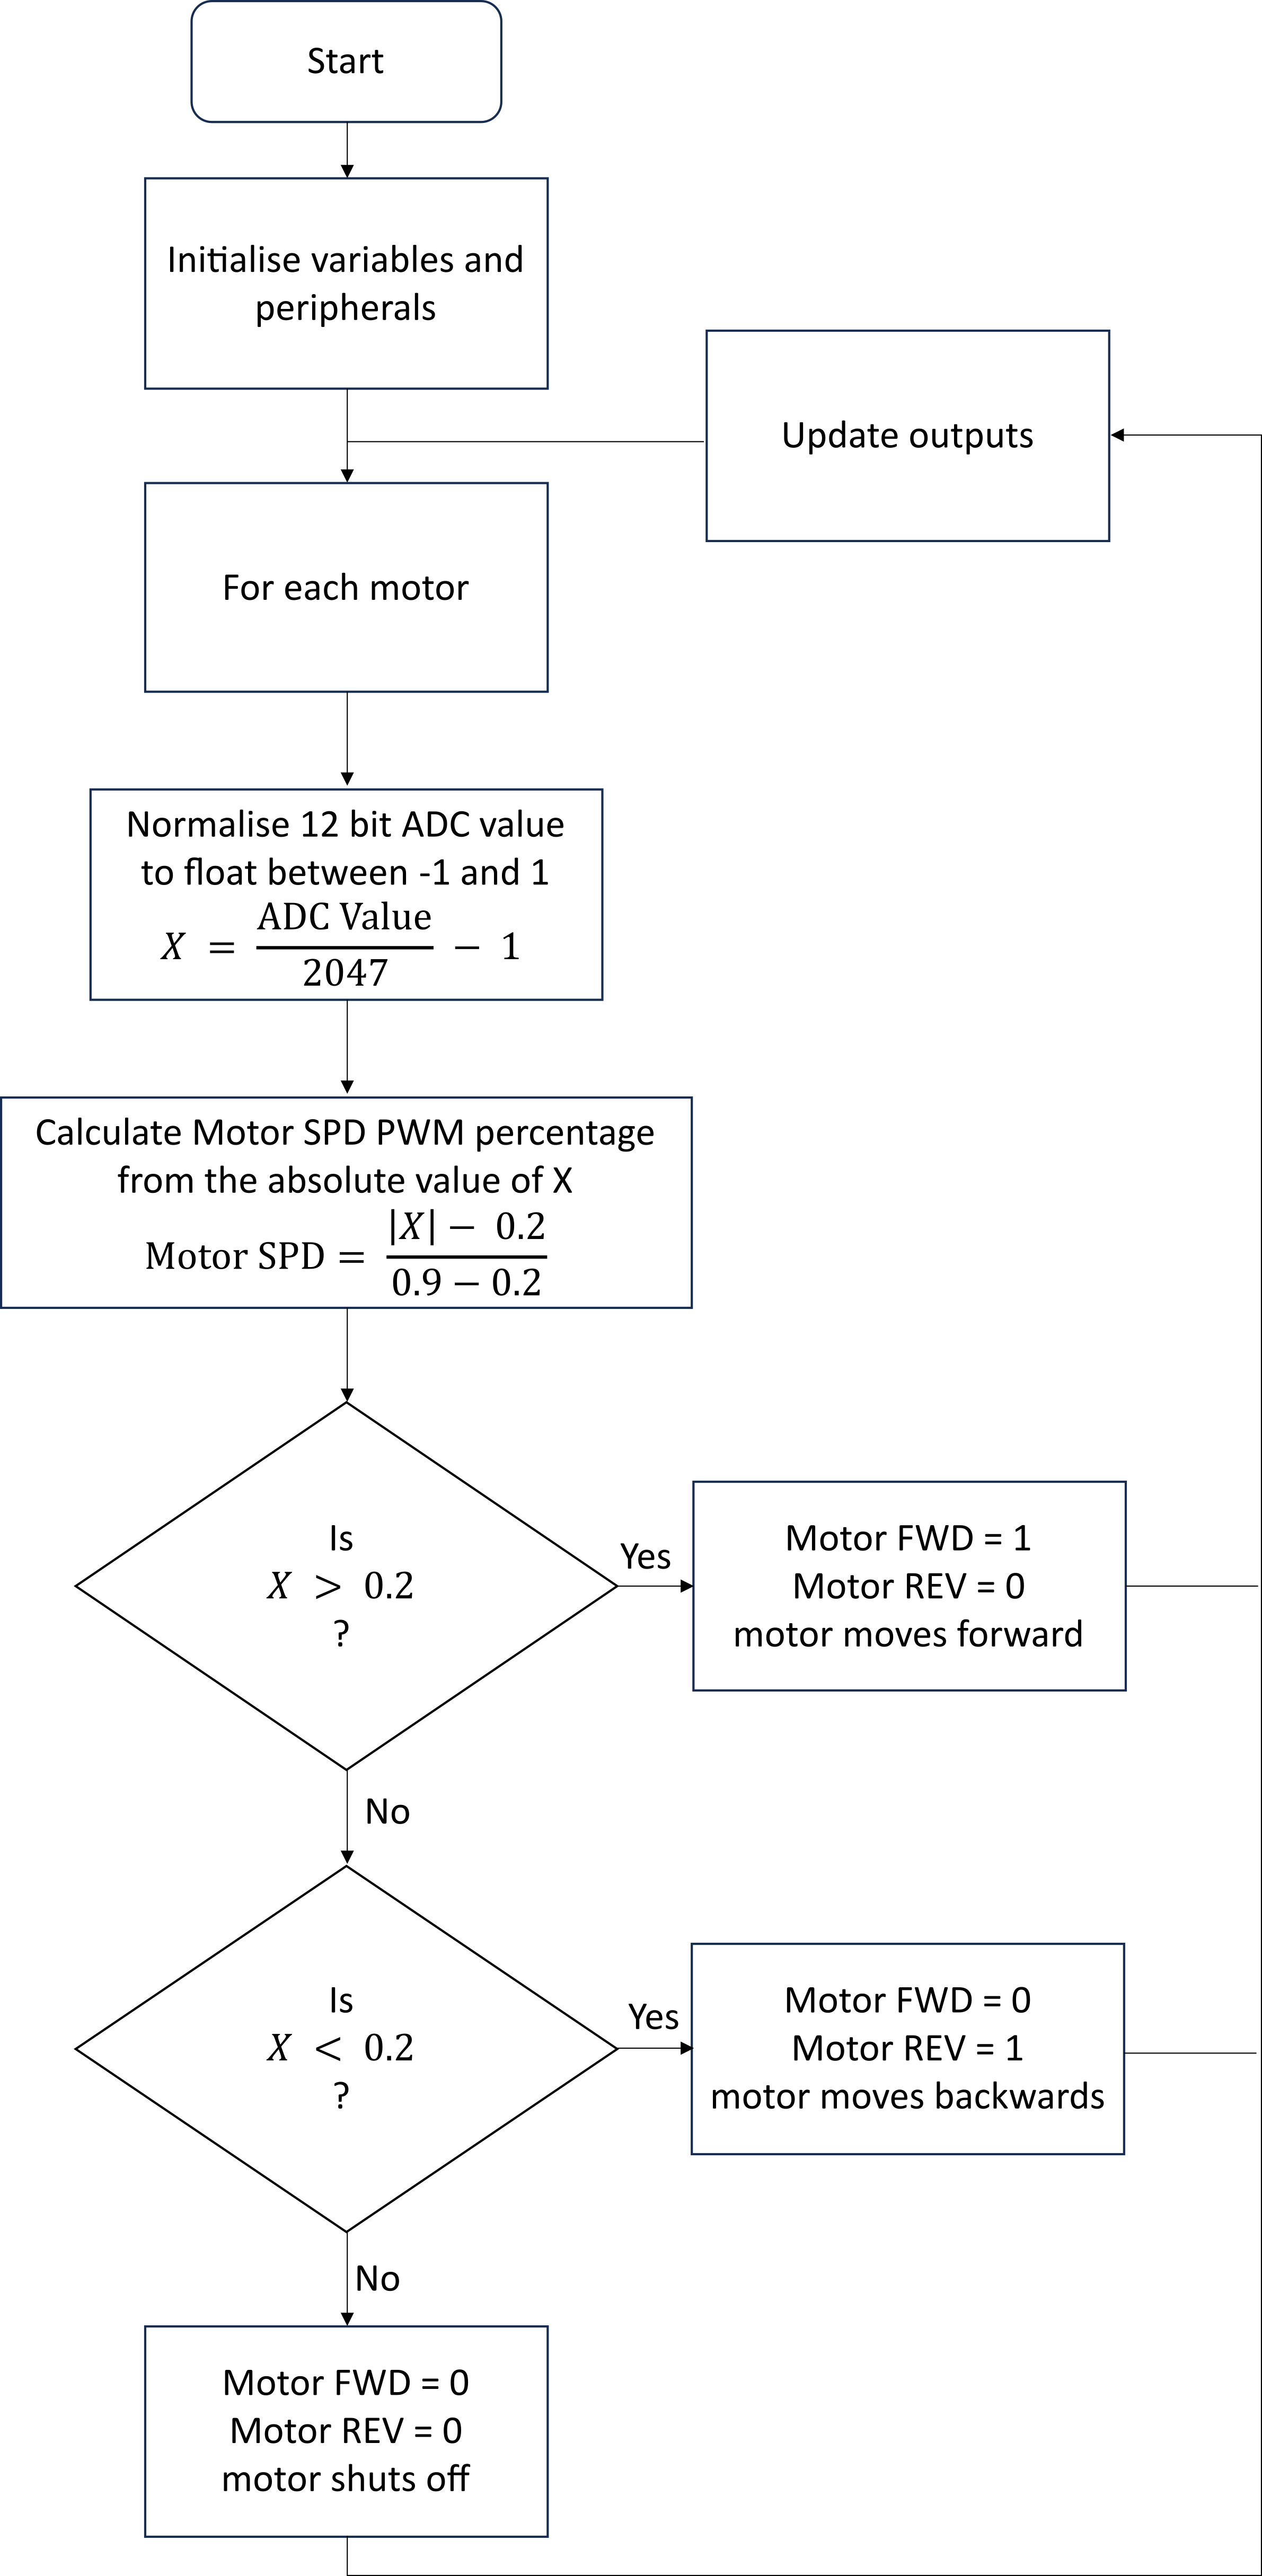
\includegraphics[height=0.6\textheight]{controller-flowchart}
	\caption{Microcontroller code flowchart.}
	\label{fig:controller-flowchart}
\end{figure}

Initial tests showed that PWM duty cycle is not proportional to torque output on the motors. Instead, even at low duty cycles, the motors can lift a large load, they just do so slowly. This is likely because the self-locking gearbox prevents the axle from ever falling backwards. Consider a DC motor lifting a lever as seen in figure ???. Typically, when the PWM signal is on, the motor outputs full torque and moves forward, then when the PWM signal is off the motor outputs no torque and falls backwards. The PWM frequency is typically high enough that the human eye sees this as a smooth motion. However, because of the self-locking gearbox, the axle will lock when the PWM signal is off rather than moving backwards, resulting in an overall forward motion even at low duty cycles. This is quite useful for controlling the motors as the speed of the motors is proportional to the PWM duty cycle regardless of the load it must lift.\\

However, for the validation of the model, the motor torque should be variable and measurable. Brushed DC motor torque is proportional to the current running through it, and the current reduces as the speed of the motor increases. The speed of the motor is also proportional to the terminal voltage. The approximate characteristics of a DC motor are given in Figure ???. The equation describing the torque of a DC motor in relation to motor voltage and speed is then,
\begin{equation}
	T = T_\mathrm{Rated-stall}(\frac{V_\mathrm{Terminal}}{V_\mathrm{Rated}}-\frac{\omega}{\omega_\mathrm{Rated-no-load}})
\end{equation}
where $T$ is the output torque, $T_\mathrm{Rated-stall}$ is the stalling torque at the rated voltage, $V_\mathrm{Terminal}$ is the supply voltage across the motor terminals, $V_\mathrm{Rated}$ is the motor's rated supply voltage, $\omega$ is the rotational speed of the output shaft, and $\omega_\mathrm{Rated-no-load}$ is the speed of the output shaft when no load is placed on it at the rated voltage.\\

\noindent To solve for the stalling torque, $\omega$ is set to $0$. This gives the relation,
\begin{equation}
	T_\mathrm{Stall} = T_\mathrm{Rated-stall}\frac{V_\mathrm{Terminal}}{V_\mathrm{Rated}}
\end{equation}
%??? Move to literature review?
In order to vary the torque of the device, the terminal voltage must be varied. For this purpose, an LM2596S buck converter is used to vary the supply voltage.

\section{Construction and testing}

\begin{wrapfigure}{r}{0.35\textwidth}
	\centering
	\includegraphics[width=0.35\textwidth]{device}
	\caption{Built device}
	\label{fig:device}
\end{wrapfigure}

To build the device, the parts were laser cut from Medium Density Fibreboard (MDF) and Acrylic. The outer surface of wheels is coated with Patex, a rubbery adhesive which is left to dry, increasing the grip of the wheels. The assembly is relatively straightforward, however it was found that the laser cut gears did not mesh well, causing them to get stuck. To address this, the teeth of the gears were filed down until they could mesh easily. This has the disadvantage of increasing kickback on the gears. However, this has little impact on performance as for all stages of motion, the gears are engaged in one direction only. The device is shown in Figure \ref{fig:device}.\\


\begin{wrapfigure}{l}{0.35\textwidth}
	\centering
	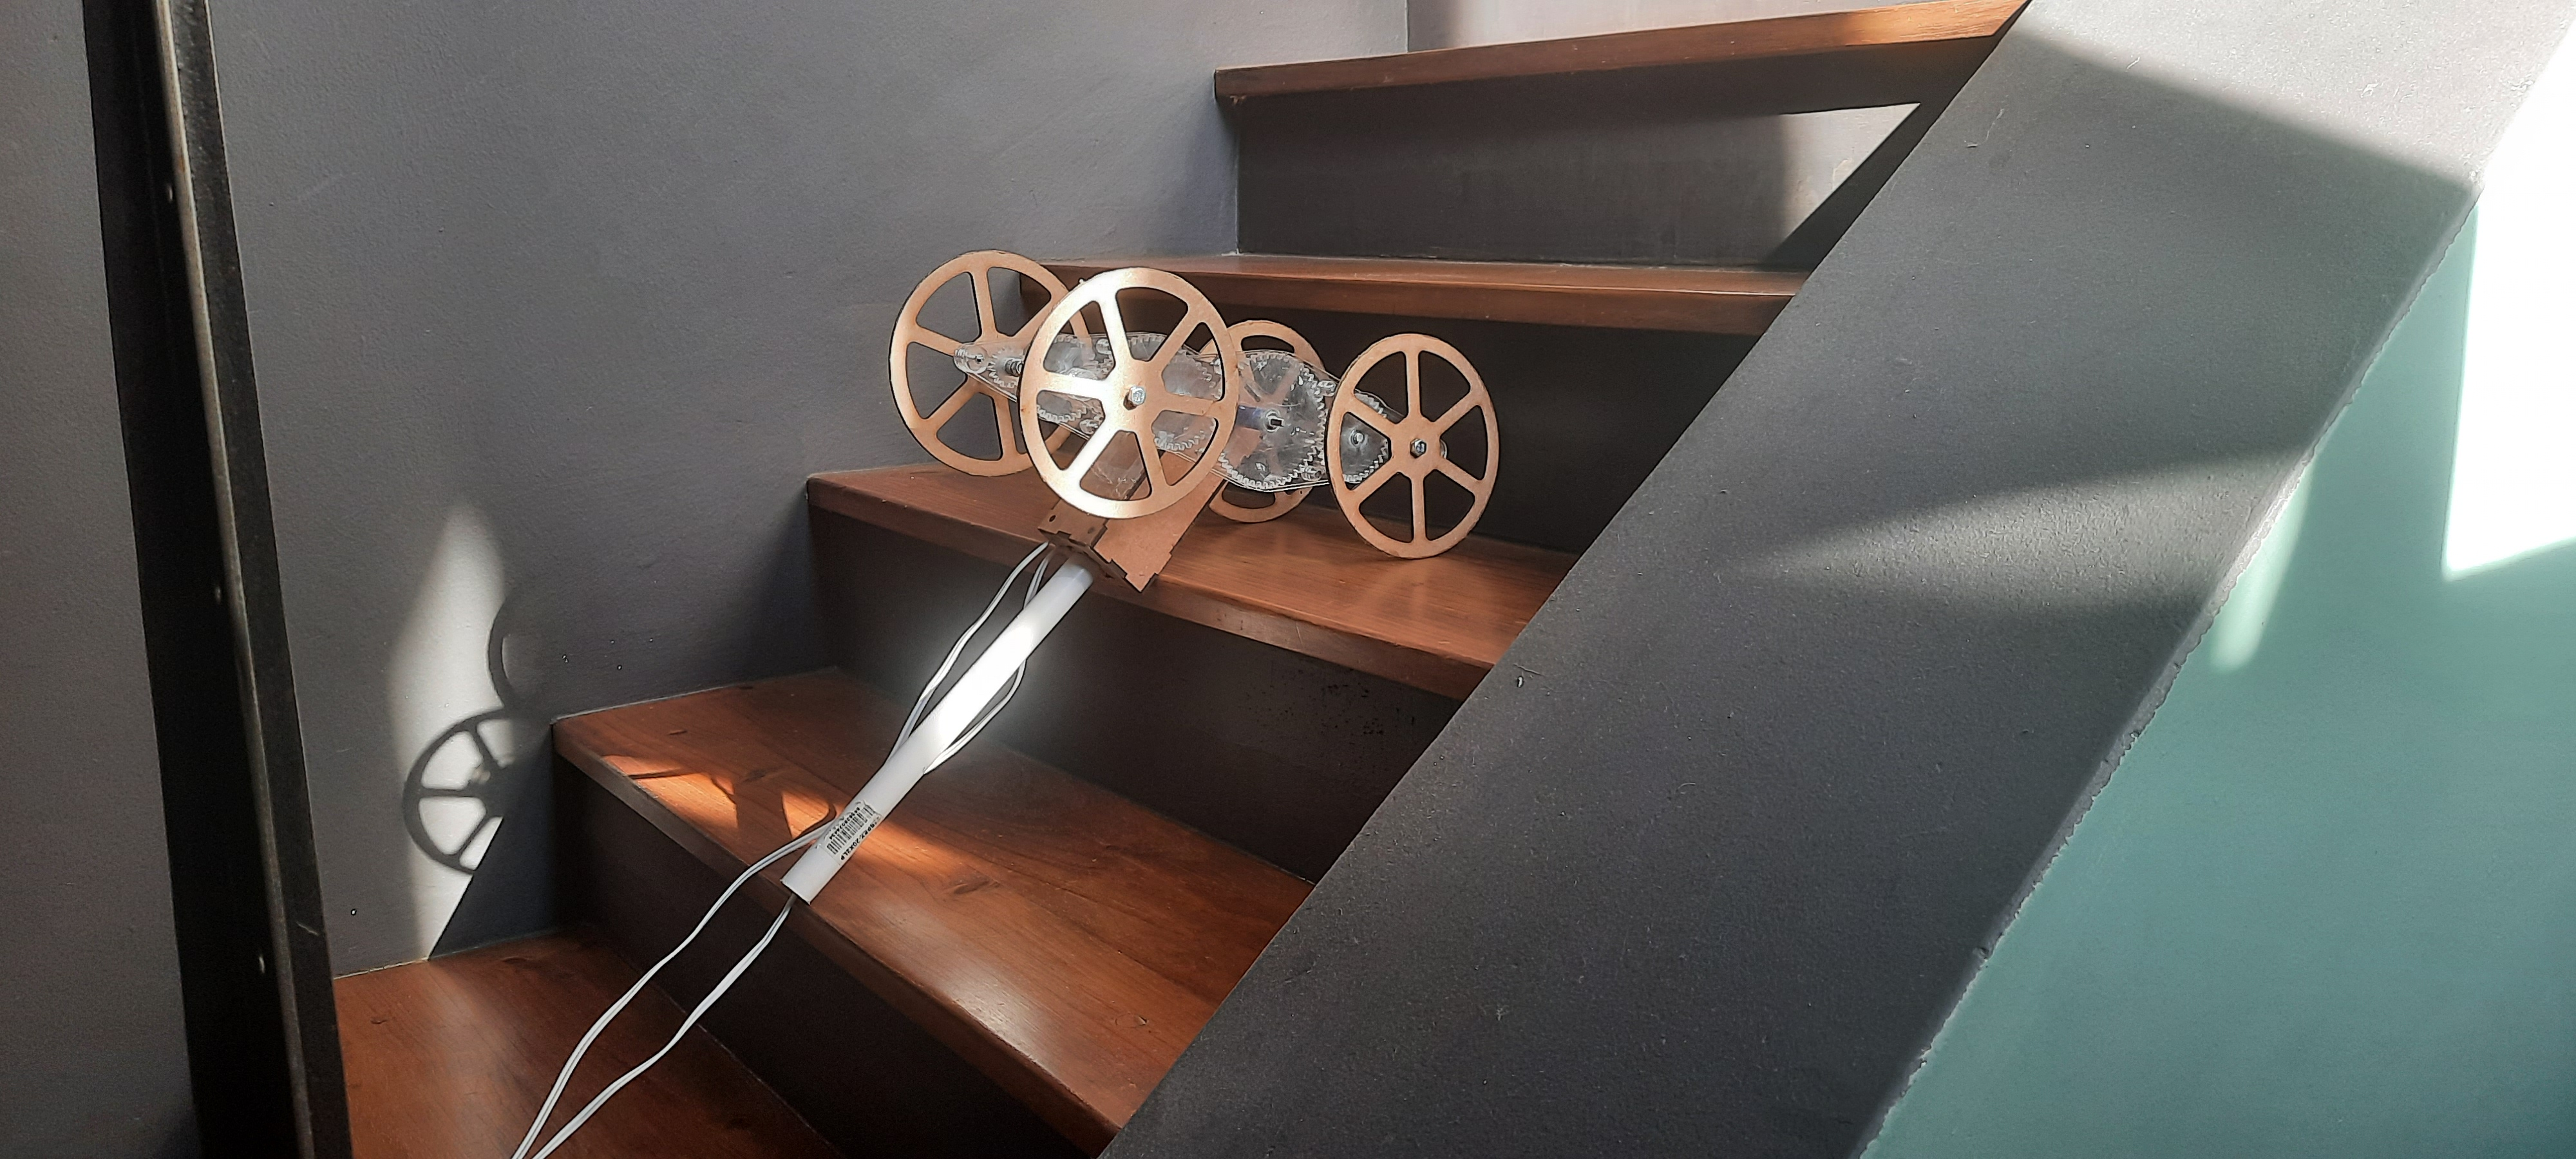
\includegraphics[width=0.35\textwidth]{device-climbing}
	\caption{Device climbing stairs}
	\label{fig:device-climbing}
\end{wrapfigure}
Initial tests show that the device is capable of climbing up two steps sequentially, which is more than any previous project achieved. This relative success can be attributed to the shorter forward protrusion of the body and possibly a higher grip on the surface of the wheels. However, the device struggled to climb a third step, this is because climbing the third step involves Stage 4 motion, which requires significantly higher torque than the previous stages. To address this, the body of the device was rebuilt using a JGY-370 gearbox motor which is geared for a higher torque. \\
After this change, the device was able to consistently climb many sequential steps, and the lower speed due to the higher gear ratio made the device easier to control during the climbing motion. Figure \ref{fig:device-climbing} shows the device climbing a flight of stairs. Initial tests also show that by applying a forward torque to one LIM and a reverse torque to the other, the device is capable of turning on the spot. However this motion is inconsistent as the LIMs can start to lift, at which point the turning stops.

%When the motor is turning it also acts as a generator, and produces a voltage known as back emf which is proportional to the speed of the motor. 
%\begin{equation}
%	E_b \propto \omega
%\end{equation}
%Where $E_b$ is the back emf and $\omega$ is the speed of the motor.
%
%The approximate circuit diagram of a DC motor is shown in figure ???. The current running through the motor is proportional to the difference between the supply voltage and the back emf.
%\begin{subequations}
%	\begin{align}
%	I &= \frac{V-E_b}{R_a
%	I &\propto V-E_b
%	\end{align}
%\end{subequations}
\chapter{Drake Simulation}

\section{Overview and objectives}

Instead of building a set of equations to simulate a robot from scratch, designers can use existing tools to simplify and streamline the modelling of a robot's movement. One such tool is rigid body simulation, which involves placing objects in a simulated environment and modelling the weights, joints, and contact forces of each object. This project uses rigid body simulation to model the motion of the device, with the objective to inform designers on how the device will move. By using established simulation software, it is easier to model the device using fewer assumptions than in the maths model, leading to a more accurate system.\\
\\
\section{Selection of simulator}
The simulation programs considered in this project are PyBullet, Gazebo, and Drake. Each of these have their own advantages but Drake was selected due to its focus on accurate multibody and friction simulation \citep{drake}.
\\
Drake is a multibody physics engine developed and used by MIT. This project uses Drake's python bindings which are available in the package "pydrake", which runs on Ubuntu using Windows Subsystem for Linux (WSL).\\
\section{CAD to simulation pipeline}
To model a robot, Drake requires a simulation description format file (SDFormat). Currently, not many CAD programs provide a method to easily generate these files. This project used Onshape, a cloud-based CAD program, for this reason. The python library, "onshape-to-robot" \citep{converter}, is then used to build an SDFormat file. The generated SDFormat file is then modified in order to meet Drake's specific requirements, and to apply realistic coefficients of friction to the wheels and tail.\\

\section{Using the simulator}
Once the robot has been loaded into the multibody simulation, it can be driven by setting a torque on the motor joints. Simply setting the torque on the joint to a constant value would cause the device to accelerate continuously ad infinitum. DC motor torque decreases as the speed increases until the torque reaches an equilibrium with the resistive forces and a constant speed is achieved. Equation \ref{eq:torqueVoltageSpeed} models the toque output of a geared DC motor.\\

\begin{equation}
	T_\mathrm{Stall} = T_\mathrm{Rated-stall}\frac{V_\mathrm{Terminal}}{V_\mathrm{Rated}} 
	\label{eq:torqueVoltageSpeed}
\end{equation}
This essentially acts as a high-gain proportional speed controller. The motor voltage is set through sliders in the simulator options. \\
The device can now be tested in simulation to determine whether it can climb stairs, and to gain insight into which components make contact with the stairs and when. Figure \ref{fig:simulation-screenshot} shows the device climbing a set of stairs in the Drake simulator.\\

\begin{figure}[h]
	\centering
	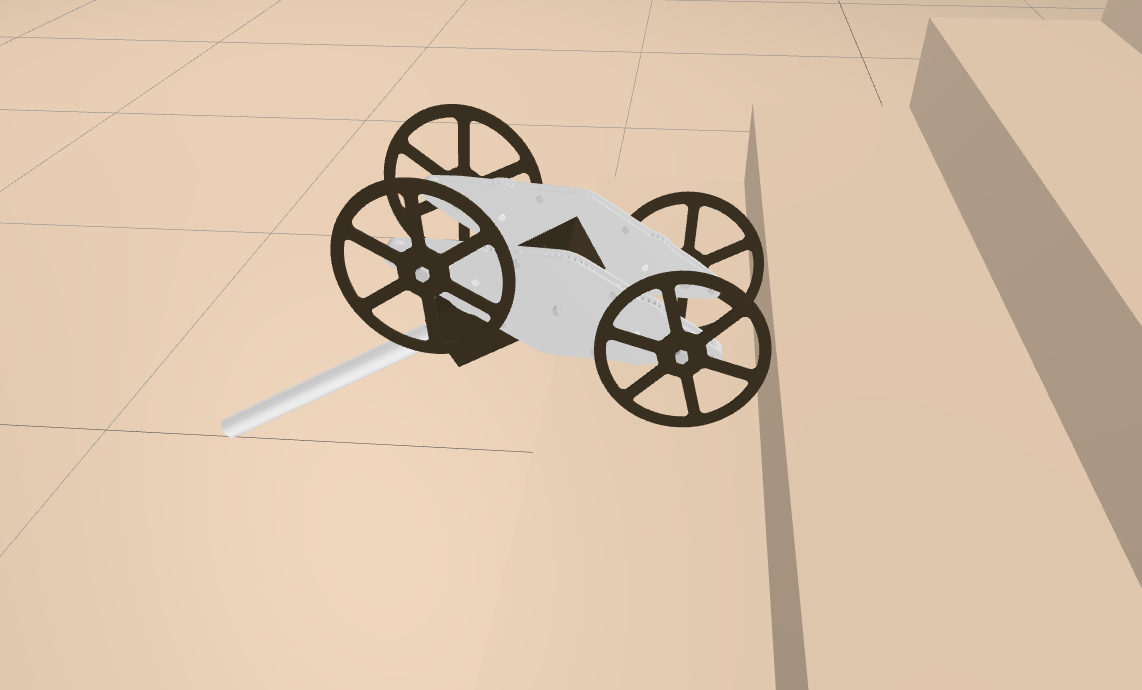
\includegraphics[width=0.8\textwidth]{simulation-screenshot}
	\caption{Screenshot of the device climbing steps in the Drake simulation.}
	\label{fig:simulation-screenshot}
\end{figure}
\chapter{Experiment}

In order to validate that the model is accurate for each motion, the torque that causes the device to perform each motion determined experimentally. The equivalent values produced by the model can be compared with the measured torques to validate the model quantitatively. However, the torque produced by a DC motor cannot be measured or set directly. The torque of a DC motor is proportional to the current running through it, and when the motor isn't moving, the current is proportional to the voltage across the motor terminals. The terminal voltage is varied in this experiment.

\section{Voltage-torque calibration}
The relationship between terminal voltage and stalling torque is determined experimentally, this will allow subsequent experiments to measure the terminal voltage and calculate the stalling torque.
To characterise the motors, an experiment was set up to determine the stalling torque produced at different input voltages. In this experiment, a the motor lifts a lever with a mass attached. The torque required to lift the lever increases as the lever angle increases, until the motor can no longer provide enough torque and stalls. The lever angle which causes the motor to stall can be used to calculate the stalling torque, specifically by using the horizontal displacement of the mass,
\begin{equation}
	T_{Stall} = m g s_x
\end{equation}
where $T_{Stall}$ is the stalling torque, $m$ is the mass attached to the lever, $g$ is the gravitational acceleration, and $s_x$ is the horizontal displacement between the mass and the motor axis.
%figure here ????
This test is repeated with different motor voltages.\\

\subsection{Variables}
Independent variable:\\
$\bullet$ Motor voltage (V)\\
Dependent variable:\\
$\bullet$ Distance the weight is lifted (mm)\\
Controlled variables:\\
$\bullet$ Motor used\\
$\bullet$ Lever used\\
$\bullet$ Power supply used\\
$\bullet$ Multimeter used\\
$\bullet$ Ruler used\\

\subsection{Method}

\begin{enumerate}
	\item Remove LIM from motor axle.
	\item Attach the lever to the motor axle.
	\item Measure the weight of the mass on a calibrated scale. \label{stepMeasure}
	\item Drive the motor until the lever is pointing straight down.
	\item Attach the mass to the lever.
	\item Adjust the voltage of the power supply to the chosen value. \label{stepAdjust}
	\item Power on the motor.
	\item Wait until the lever stops moving.
	\item Record the voltage across the motor terminals. 
	\item Quickly power off the motor. Leaving the motor on while stalling can cause damage to the motor.
	\item Measure the horizontal distance that the lever has moved.
	\item Drive the motor until the lever is pointing straight down. \label{stepReset}
	\item Repeat steps \ref{stepAdjust} to \ref{stepReset} with different power supply voltages.
	\item Remove the mass from the lever. \label{stepRemove}
	\item Repeat steps \ref{stepMeasure} to \ref{stepRemove} with different masses.
\end{enumerate}
\subsection{Results}
The measured results, as well as the calculated torque, are shown in Table \ref{voltage-torque-table}, and visualised in Figure \ref{torque-voltage-plot}.

\begin{table}[!ht]
	\label{voltage-torque-table}
	\centering
	\begin{tabular}{|l|l|l|l|}
		\hline
		Mass (g) & Lever (mm) & Voltage (V) & Torque (Nm) \\ \hline
		145 & 97 & 0.83 & 0.13797765 \\ \hline
		145 & 101 & 0.92 & 0.14366745 \\ \hline
		145 & 151 & 1.1 & 0.21478995 \\ \hline
		204 & 154 & 1.22 & 0.30819096 \\ \hline
		204 & 229 & 1.56 & 0.45828396 \\ \hline
		542 & 89 & 1.72 & 0.47321478 \\ \hline
		537 & 106 & 1.93 & 0.55840482 \\ \hline
		542 & 106 & 1.8 & 0.56360412 \\ \hline
		537 & 164 & 2.45 & 0.86394708 \\ \hline
		542 & 171 & 2.5 & 0.90921042 \\ \hline
		542 & 220 & 3 & 1.1697444 \\ \hline
		542 & 242 & 3.25 & 1.28671884 \\ \hline
		1289 & 117 & 3.5 & 1.47947553 \\ \hline
		1289 & 136 & 4 & 1.71973224 \\ \hline
		1289 & 160 & 4.5 & 2.0232144 \\ \hline
	\end{tabular}
\end{table}

\begin{figure}[!h]
	\centering
	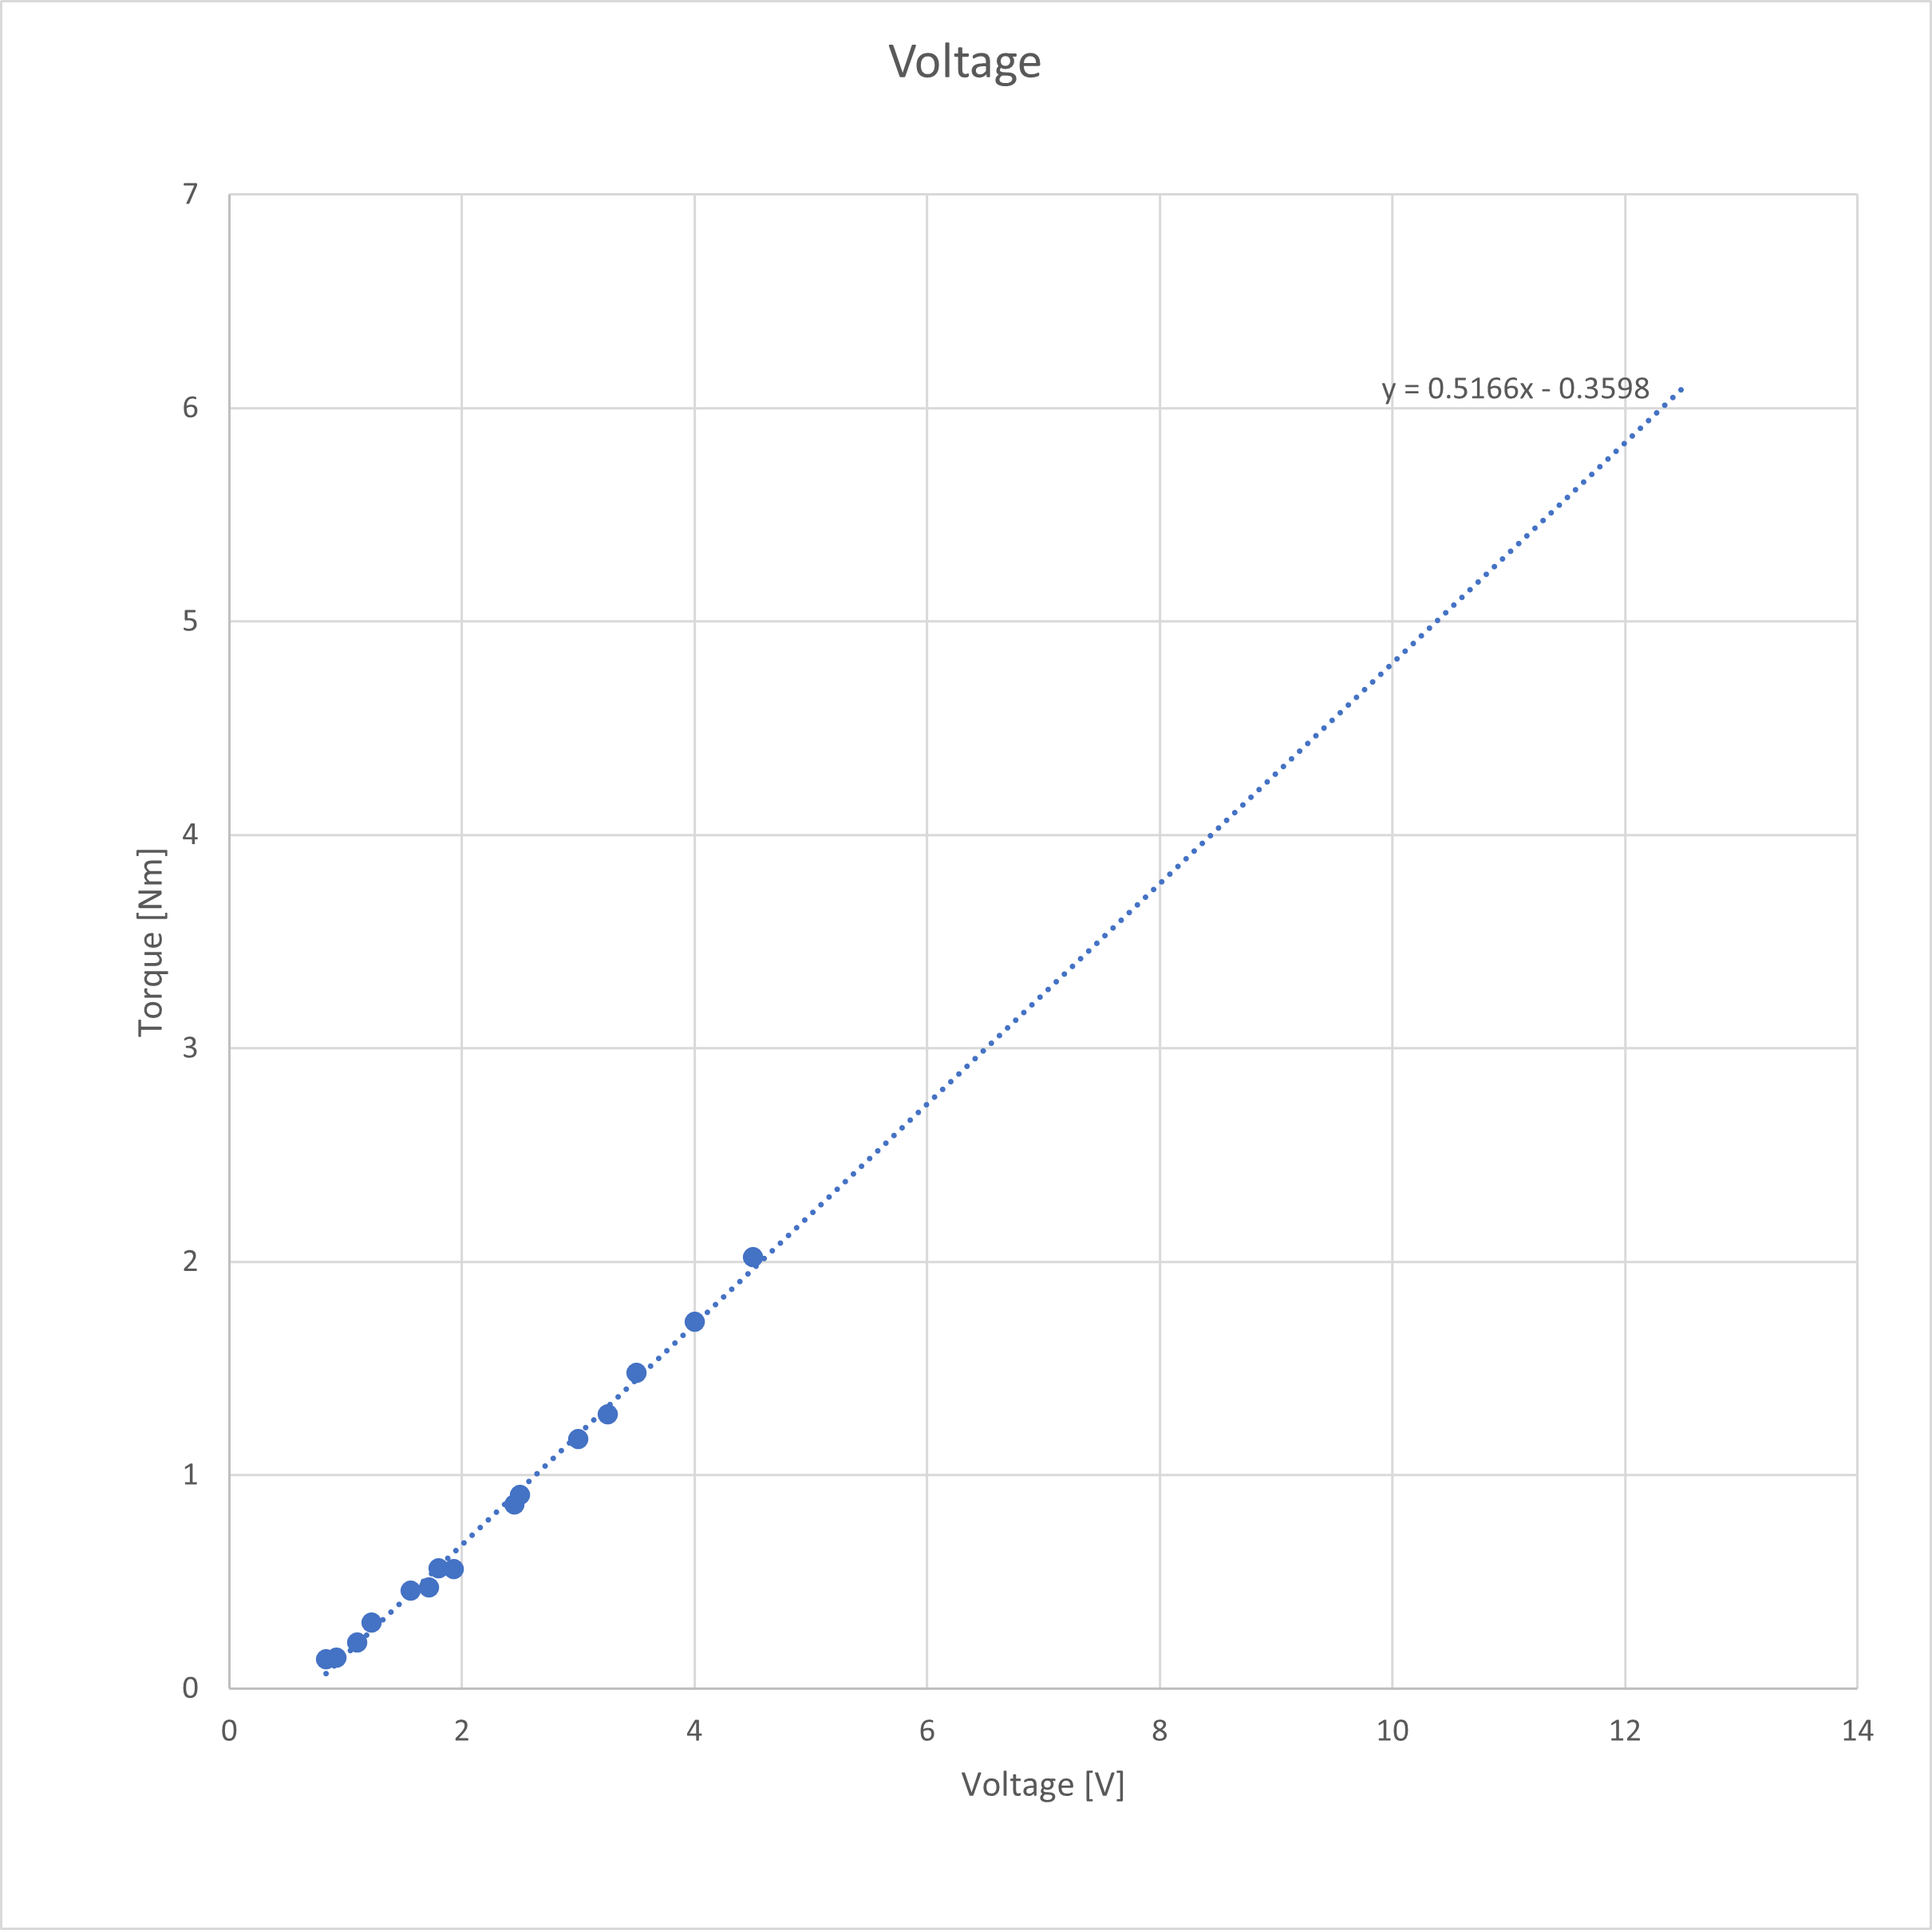
\includegraphics[width=0.8\textwidth]{plots/torque-voltage-relation.png}
	\caption{Relationship between motor voltage and stalling torque.}
	\label{torque-voltage-plot}
\end{figure}

This plot shows a linear relationship between stalling torque and voltage, and gives the formula,
\begin{equation}
	T_{Stall} =  0.5166 V - 0.3598 \label{eqTorqueVoltage}
\end{equation}
where $V$ is the motor terminal voltage.
This experiment did not attempt to measure torques beyond $2 Nm$ as this risked damaging the device and was beyond the expected requirements for the device.



\section{Climbing torque}
This experiment aims to determine the torque required to lift the device through each stage of motion. The results of this experiment will be compared with the compared with the theoretical torques required provided by the model and the simulation. The device is placed in the starting position for each stage of motion and powered with a certain supply voltage. The motion of the device is then assessed, if the device does not move then it is marked as "None"; if the device starts to move but does not complete the stage of motion, it is marked as "Partial"; and if it completes the stage of motion, it is marked as "Full".\\

%???? figure here

\subsection{Variables}
Independent variable:\\
$\bullet$ Motor voltage (V)\\
Dependent variable:\\
$\bullet$ Assessment of motion ("Full", "Partial", or "None")\\
Controlled variables:\\
$\bullet$ LIMed device\\
$\bullet$ Stairs\\
$\bullet$ Multimeter used\\


\subsection{Method}

\begin{enumerate}
	\item Place device in the starting position for the chosen stage of motion. \label{stepPlace}
	\item Adjust the voltage of the power supply to the chosen value.
	\item Power on the device.
	\item Observe how the device moves and classify the movement into "Full", "Partial", or "None". 
	\item Record the voltage across the motor terminals. 
	\item Power off the device.\label{stepOff}
	\item Repeat steps \ref{stepPlace} to \ref{stepOff} with a range of power supply voltages.\label{stepRepeatVoltage}
	\item Repeat steps \ref{stepPlace} to \ref{stepRepeatVoltage} for the different stages of motion.
\end{enumerate}

\subsection{Results}

Table \ref{tableStage1Torque} shows the measured results for the Stage 1 motion, as well as the torques calculated using Equation \ref{eqTorqueVoltage}. The data for the other stages of motion can be found in Appendix ???.

\begin{table}[!h]
	\caption{Torque experiment results for Stage 1}
	\label{tableStage1Torque}
	\centering
	\begin{tabular}{|l|l|l|}
		\hline
		Voltage (V) & Assessment of motion & Torque (Nm) \\ \hline
		0.89 & None & 0.099974 \\ \hline
		1.08 & None & 0.198128 \\ \hline
		1.12 & None & 0.218792 \\ \hline
		1.57 & None & 0.451262 \\ \hline
		1.68 & None & 0.508088 \\ \hline
		1.74 & None & 0.539084 \\ \hline
		1.81 & None & 0.575246 \\ \hline
		1.87 & None & 0.606242 \\ \hline
		1.89 & Partial & 0.616574 \\ \hline
		1.98 & Partial & 0.663068 \\ \hline
		2.05 & Partial & 0.69923 \\ \hline
		2.11 & Full & 0.730226 \\ \hline
		2.13 & Full & 0.740558 \\ \hline
		2.25 & Full & 0.80255 \\ \hline
		2.26 & Full & 0.807716 \\ \hline
		2.3 & Full & 0.82838 \\ \hline
	\end{tabular}
\end{table}

This data is plotted in Figure \ref{plotassessment-torque-relation-stage1}, which shows that the full motion only happens with torques of at least $0.73 Nm$, while partial motion only requires $0.61 Nm$.

\begin{figure}[h]
	\centering
	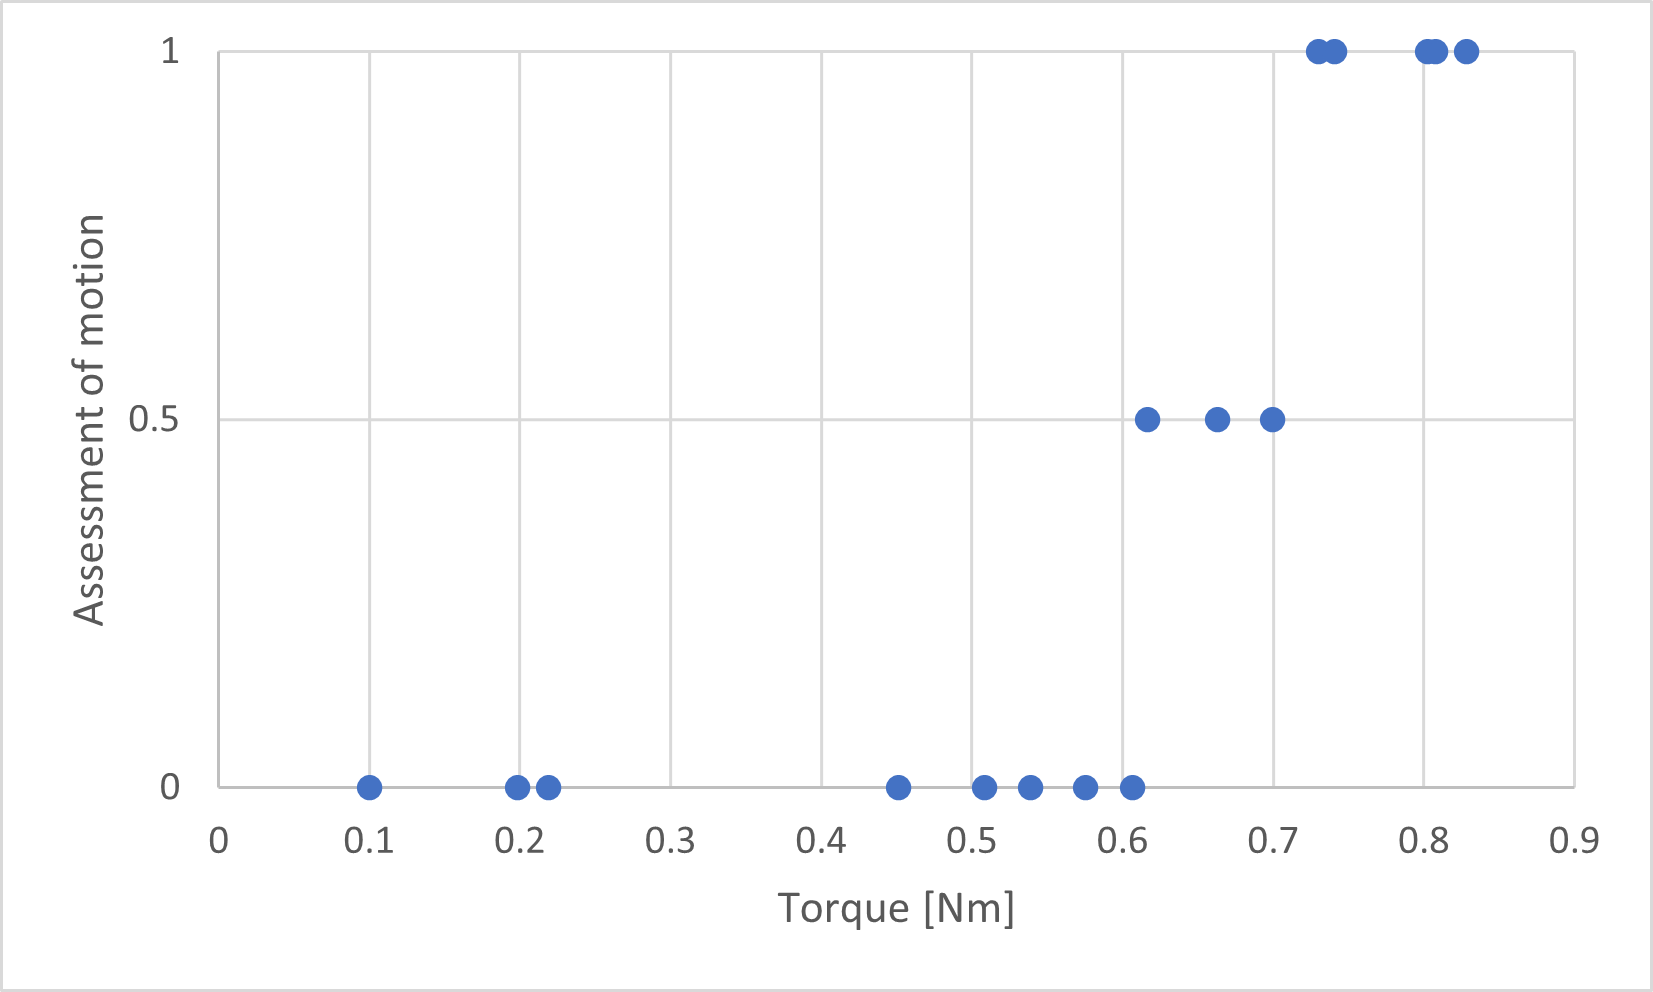
\includegraphics[width=0.8\textwidth]{plots/assessment-torque-relation-stage1}
	\caption{Relationship between torque and motion for Stage 1, with 0, 0.5, and 1 representing "None", "Partial", and "Full" respectively.}
	\label{plotassessment-torque-relation-stage1}
\end{figure}



\chapter{Analysis}

The objective of this analysis is to validate the model and the simulation. The values calculated in the maths model and simulated in Drake are compared with the experimental data to determine the validity of the maths model and the simulation.

\section{Qualitative comparison}

The motor torque over time for Stage 1 motion was recorded during the Drake simulation, and is shown in Figure \ref{fig:torque-stage-1}. This shows a similar curve to the plot of recorded current, which is shown again in Figure \ref{fig:current-2}. The simulation completed Stage 1 in 2.8 s, which is faster than the real device which took 3.25 s. The noise in the simulated data is due to oscillations caused by Equation \ref{eq:torqueVoltageSpeed}, which acts as a proportional feedback controller on the speed in the simulation. This oscillation could be reduced by decreasing the simulation time step, however this would proportionally increase the simulation time taken, and a low time step of 0.01 ms is already selected. Both plots show a large spike as the motors are powered on and a slight dip before Stage 1 completes. This indicates that the torque produced by the device throughout the simulation accurately matches the torque that the real device would produce.
\begin{figure}[!ht]
	\centering
	\begin{subfigure}{.5\textwidth}
		\centering
		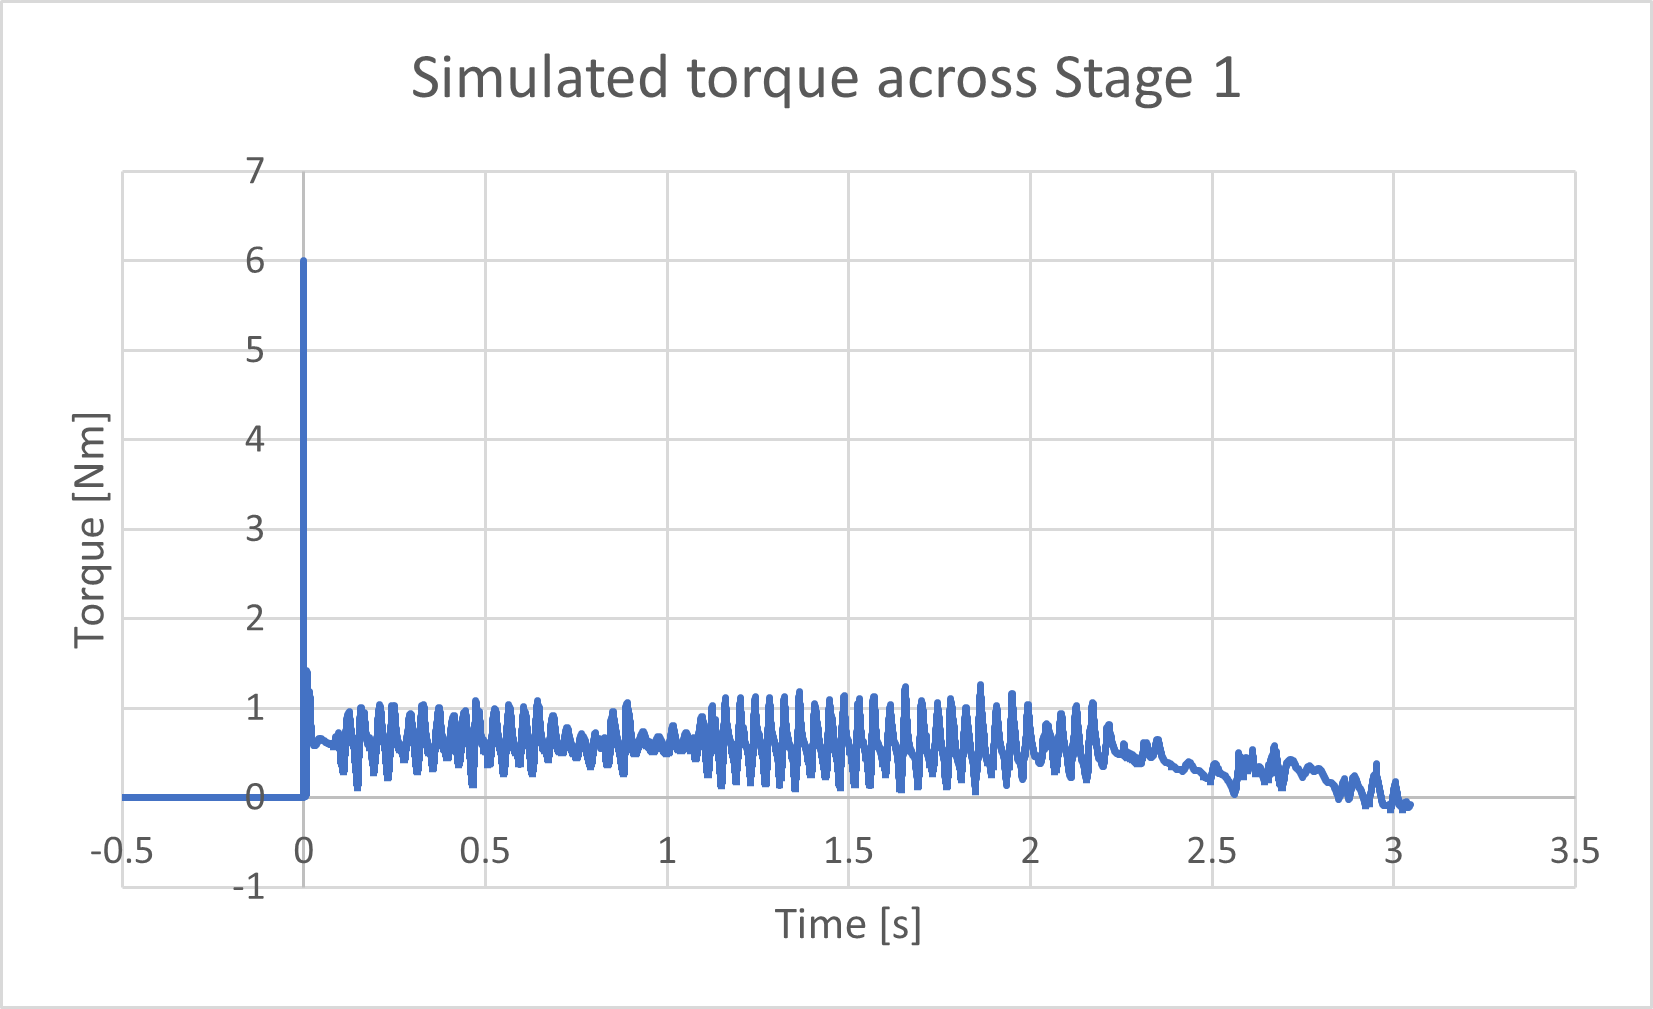
\includegraphics[width=.9\linewidth]{plots/torque-stage-1}
		\caption{Torque recorded over time as the \\simulated device completes Stage 1.}
		\label{fig:torque-stage-1}
	\end{subfigure}%
	\begin{subfigure}{.5\textwidth}
		\centering
		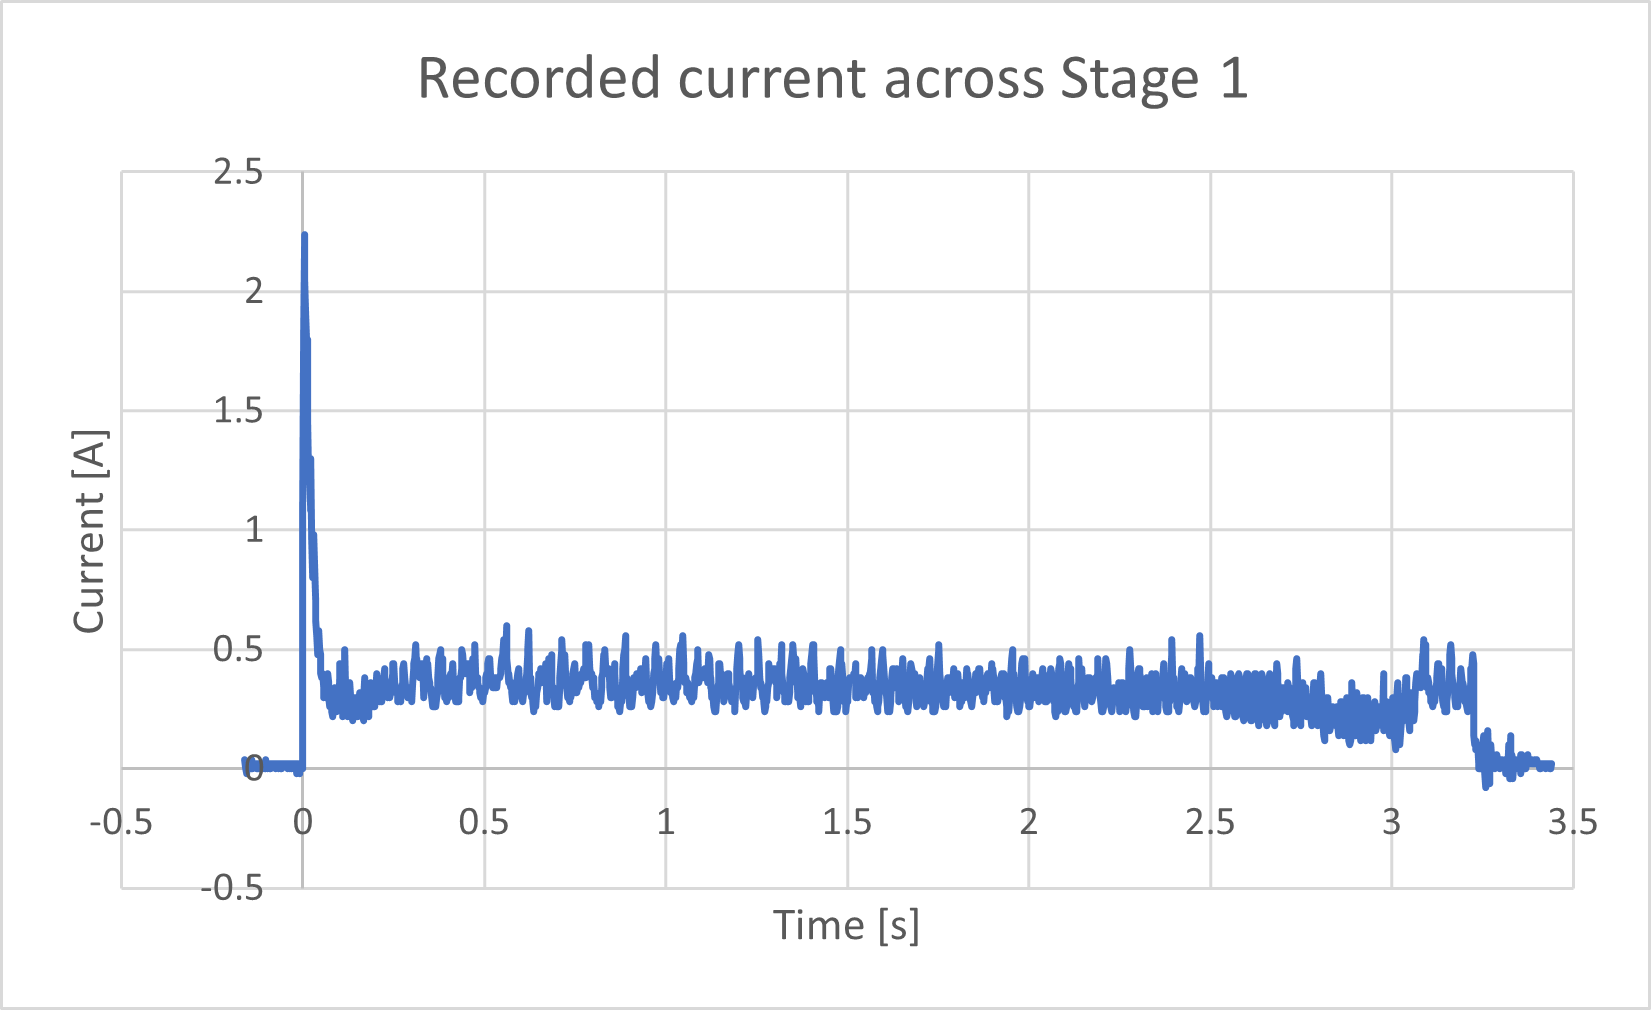
\includegraphics[width=.9\linewidth]{plots/current-stage-1}
		\caption{Current recorded over time as the device completes Stage 1.}
		\label{fig:current-2}
	\end{subfigure}
	\caption{Simulated current and recorded torque.}
	\label{fig:torque-current}
\end{figure}


\section{Quantitative comparison}

The torque measurement experiment gives two values for each stage of motion, the torque required to cause some partial movement, and the torque required to cause full movement. These values will be referred to as $T_\mathrm{Partial}$ and $T_\mathrm{Full}$ respectively, and are shown in Figure \ref{fig:torque-experiment}.

\begin{figure}[!h]
	\centering
	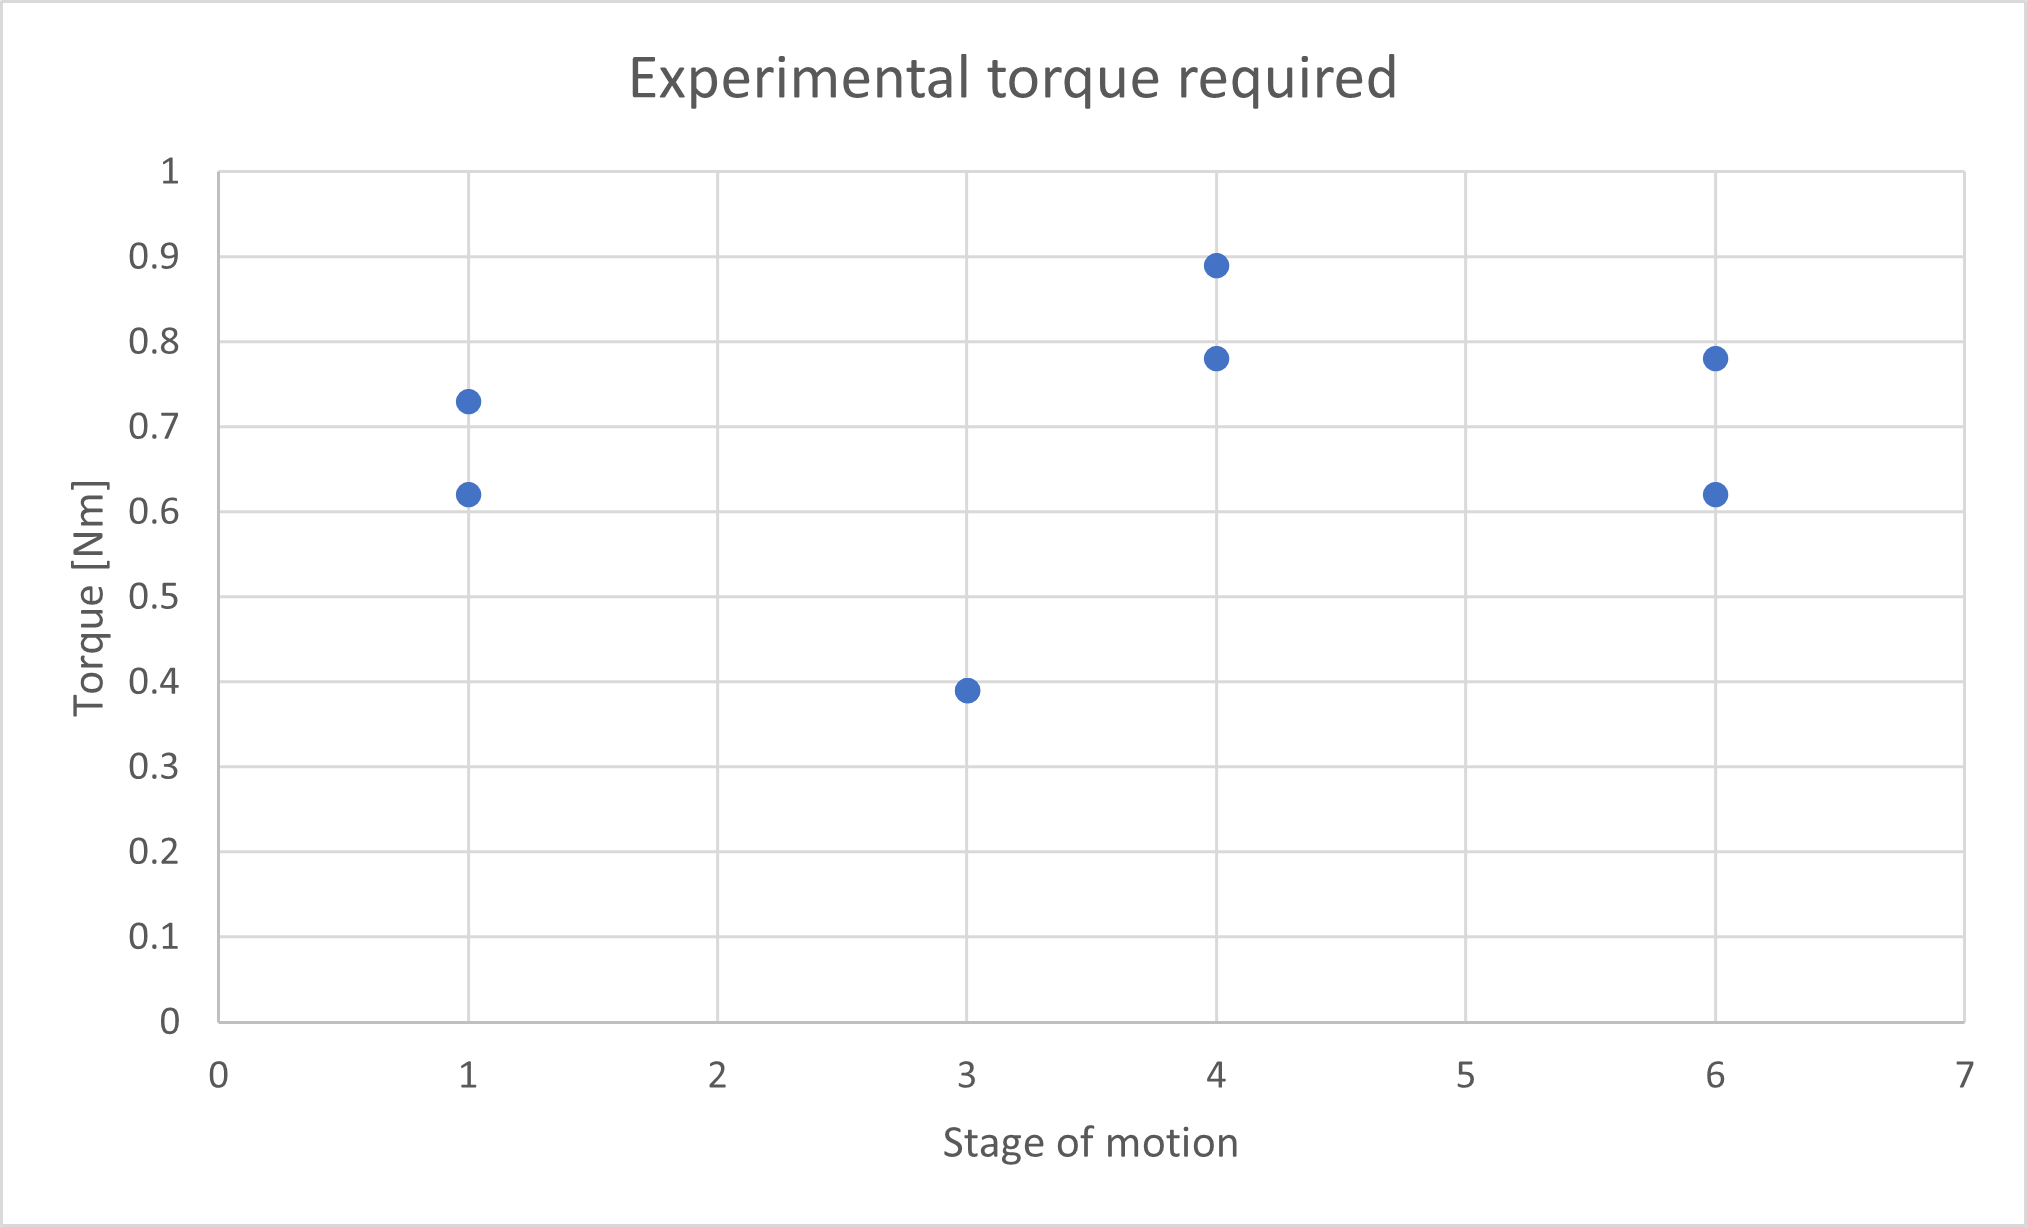
\includegraphics[width=0.8\textwidth]{plots/torque-experiment}
	\caption{Required torques for each stage determined experimentally}
	\label{fig:torque-experiment}
\end{figure}

In Figure \ref{fig:torque-experiment}, there are two points for each stage, the higher of which is $T_\mathrm{Full}$ and the lower is $T_\mathrm{Partial}$. In cases where only a single point is present, there was no torque that would cause a partial movement; meaning that if the torque is high enough to start the movement, it is also high enough to complete the movement. Stages 0, 2, and 5 are omitted as the device does not push against gravity in these stages, so the torque required is negligible.\\

To determine the required torque in the simulation, the torque measurement experiment is simulated. The torque required across each stage of motion has already been calculated using the maths model, as shown in Figure \ref{fig:bigplot}. The required torque at the start of each stage is equivalent to $T_\mathrm{Partial}$, as this is the torque that will cause the motion to start. The highest required torque for each stage is $T_\mathrm{Full}$, because if the device can output this torque it will be able to complete the full stage of motion. The required torque produced by the simulation and the maths model are shown side by side with the experimental data in Figure \ref{fig:torque-comparison}.\\

\begin{figure}[!h]
	\centering
	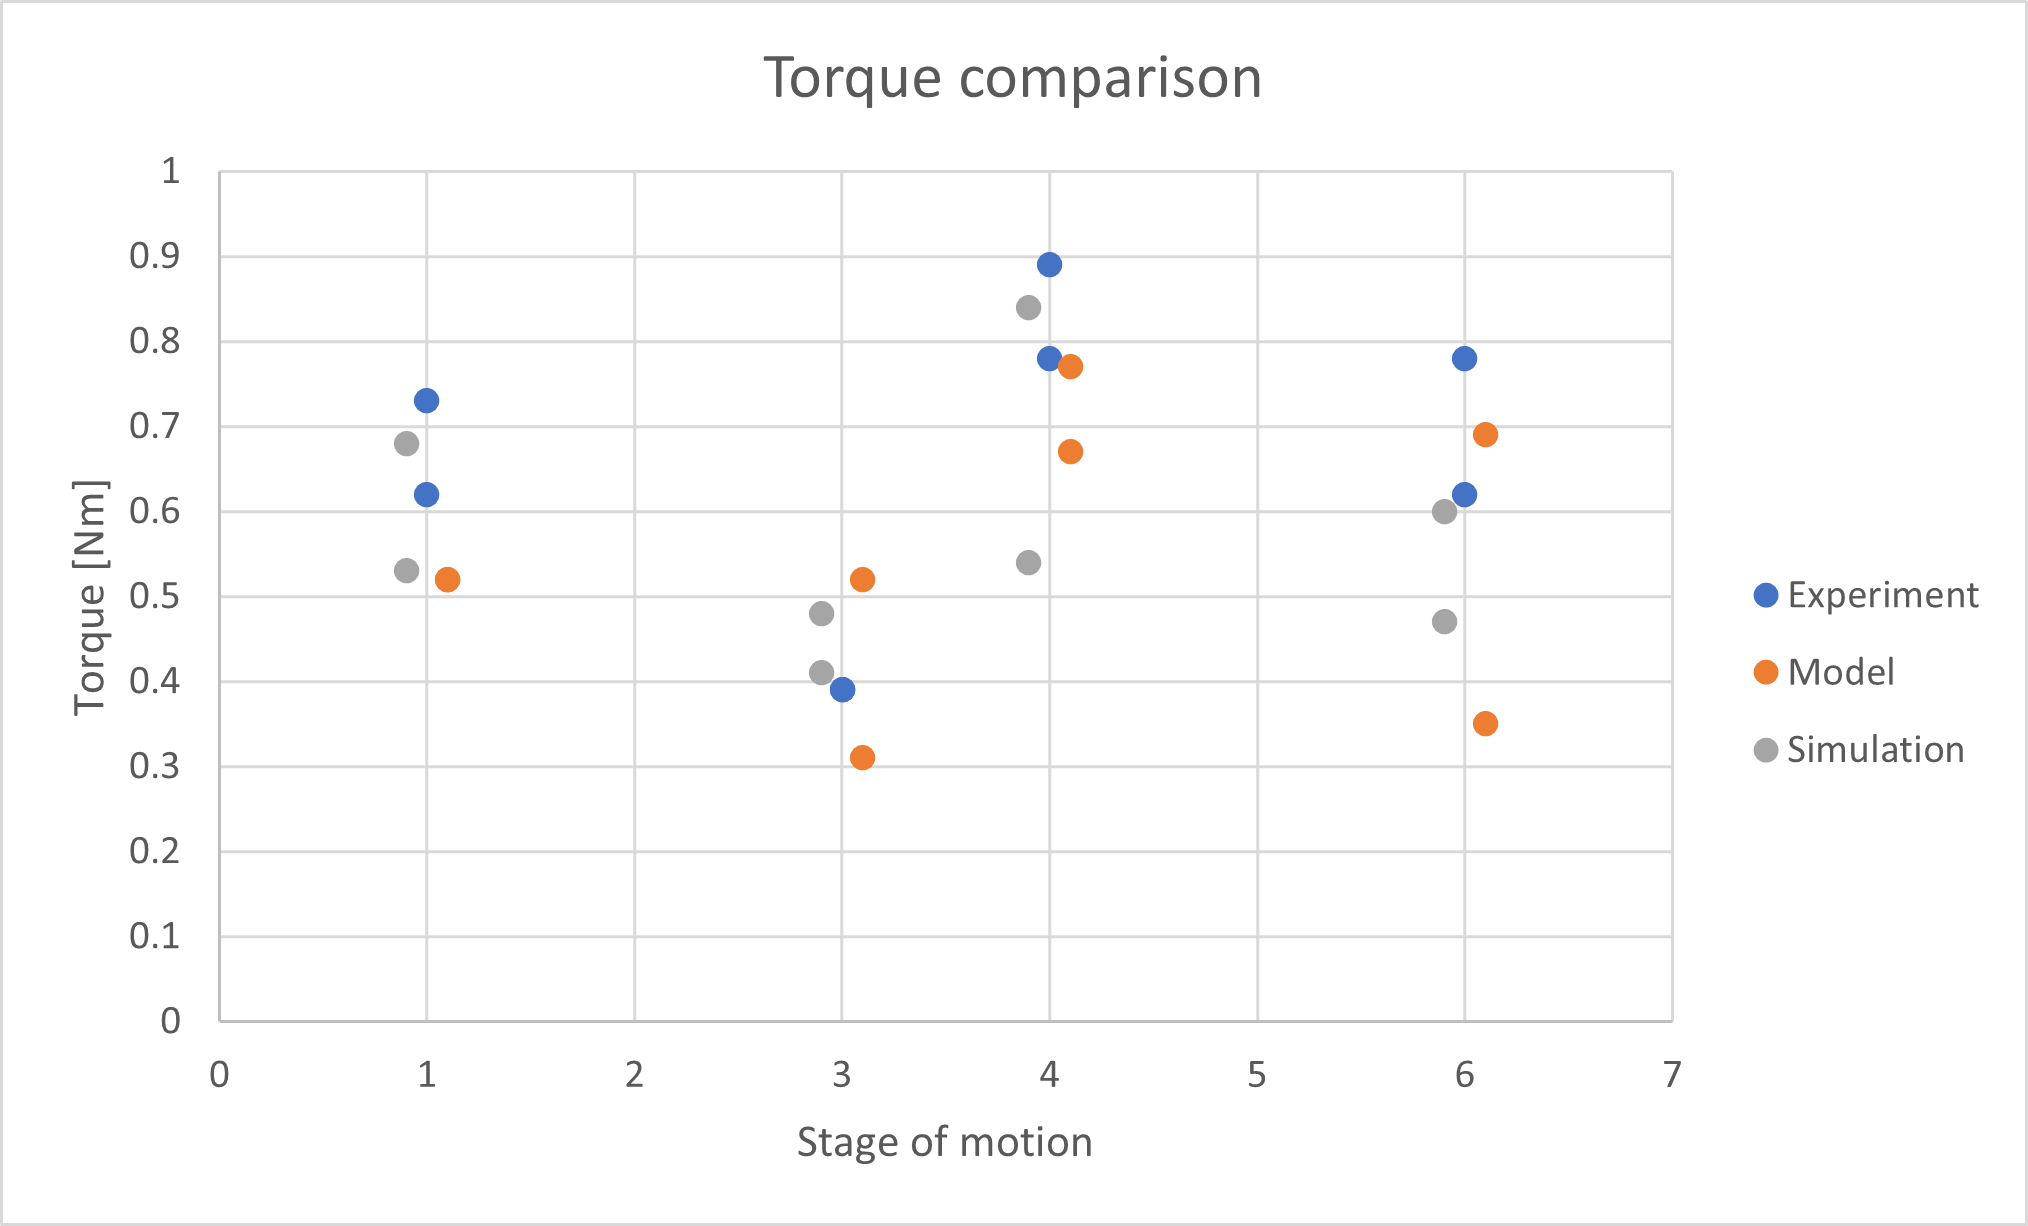
\includegraphics[width=0.8\textwidth]{plots/torque-comparison}
	\caption{Required torques for each stage from different sources.}
	\label{fig:torque-comparison}
\end{figure}

Figure \ref{fig:torque-comparison} shows that the model, simulation, and experiment all show similar trends but produce different values. In Stages 1, 4, and 6, the model and simulation both produce a lower required torque than the device actually needs. In Stage 3, the device needs less torque to complete the motion than the model and simulation predict.\\
To test the accuracy of the model and simulation across a range of design parameters, the experiment and comparison were repeated twice, once with a 60 cm long tail in place of the 30 cm one, and once with a 340 g mass attached to the body of the device. The comparison between these results are shown in Figures \ref{fig:torque-comparison-tail} and \ref{fig:torque-comparison-mass}. These plots show similar trends, indicating that the model and simulation give consistent results for a range of design parameters.

\begin{figure}
	\centering
	\begin{subfigure}{.5\textwidth}
		\centering
		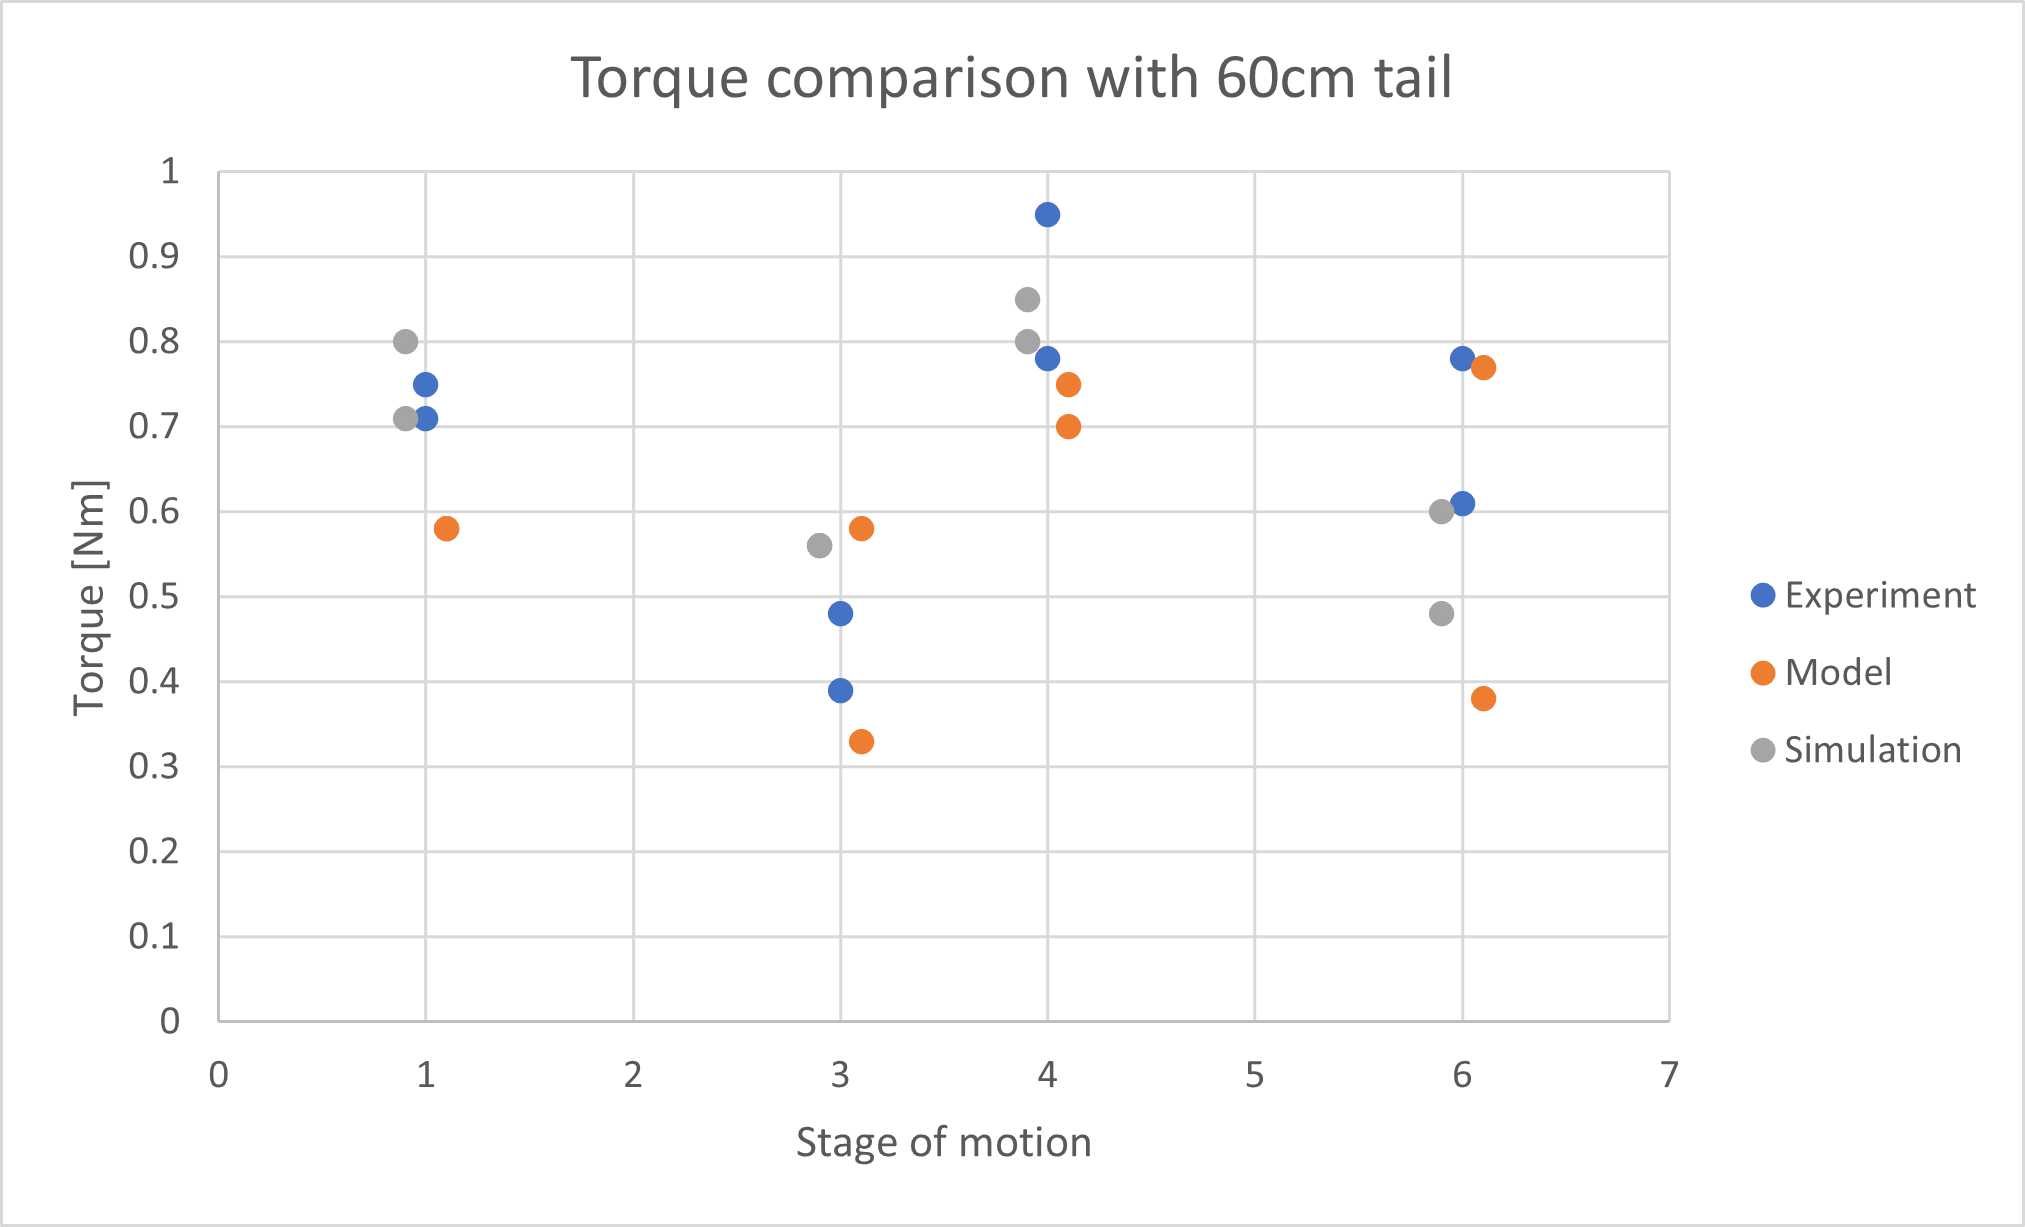
\includegraphics[width=.9\linewidth]{plots/torque-comparison-tail}
		\caption{Required torques for each stage when \\device has a 60 cm tail.}
		\label{fig:torque-comparison-tail}
	\end{subfigure}%
	\begin{subfigure}{.5\textwidth}
		\centering
		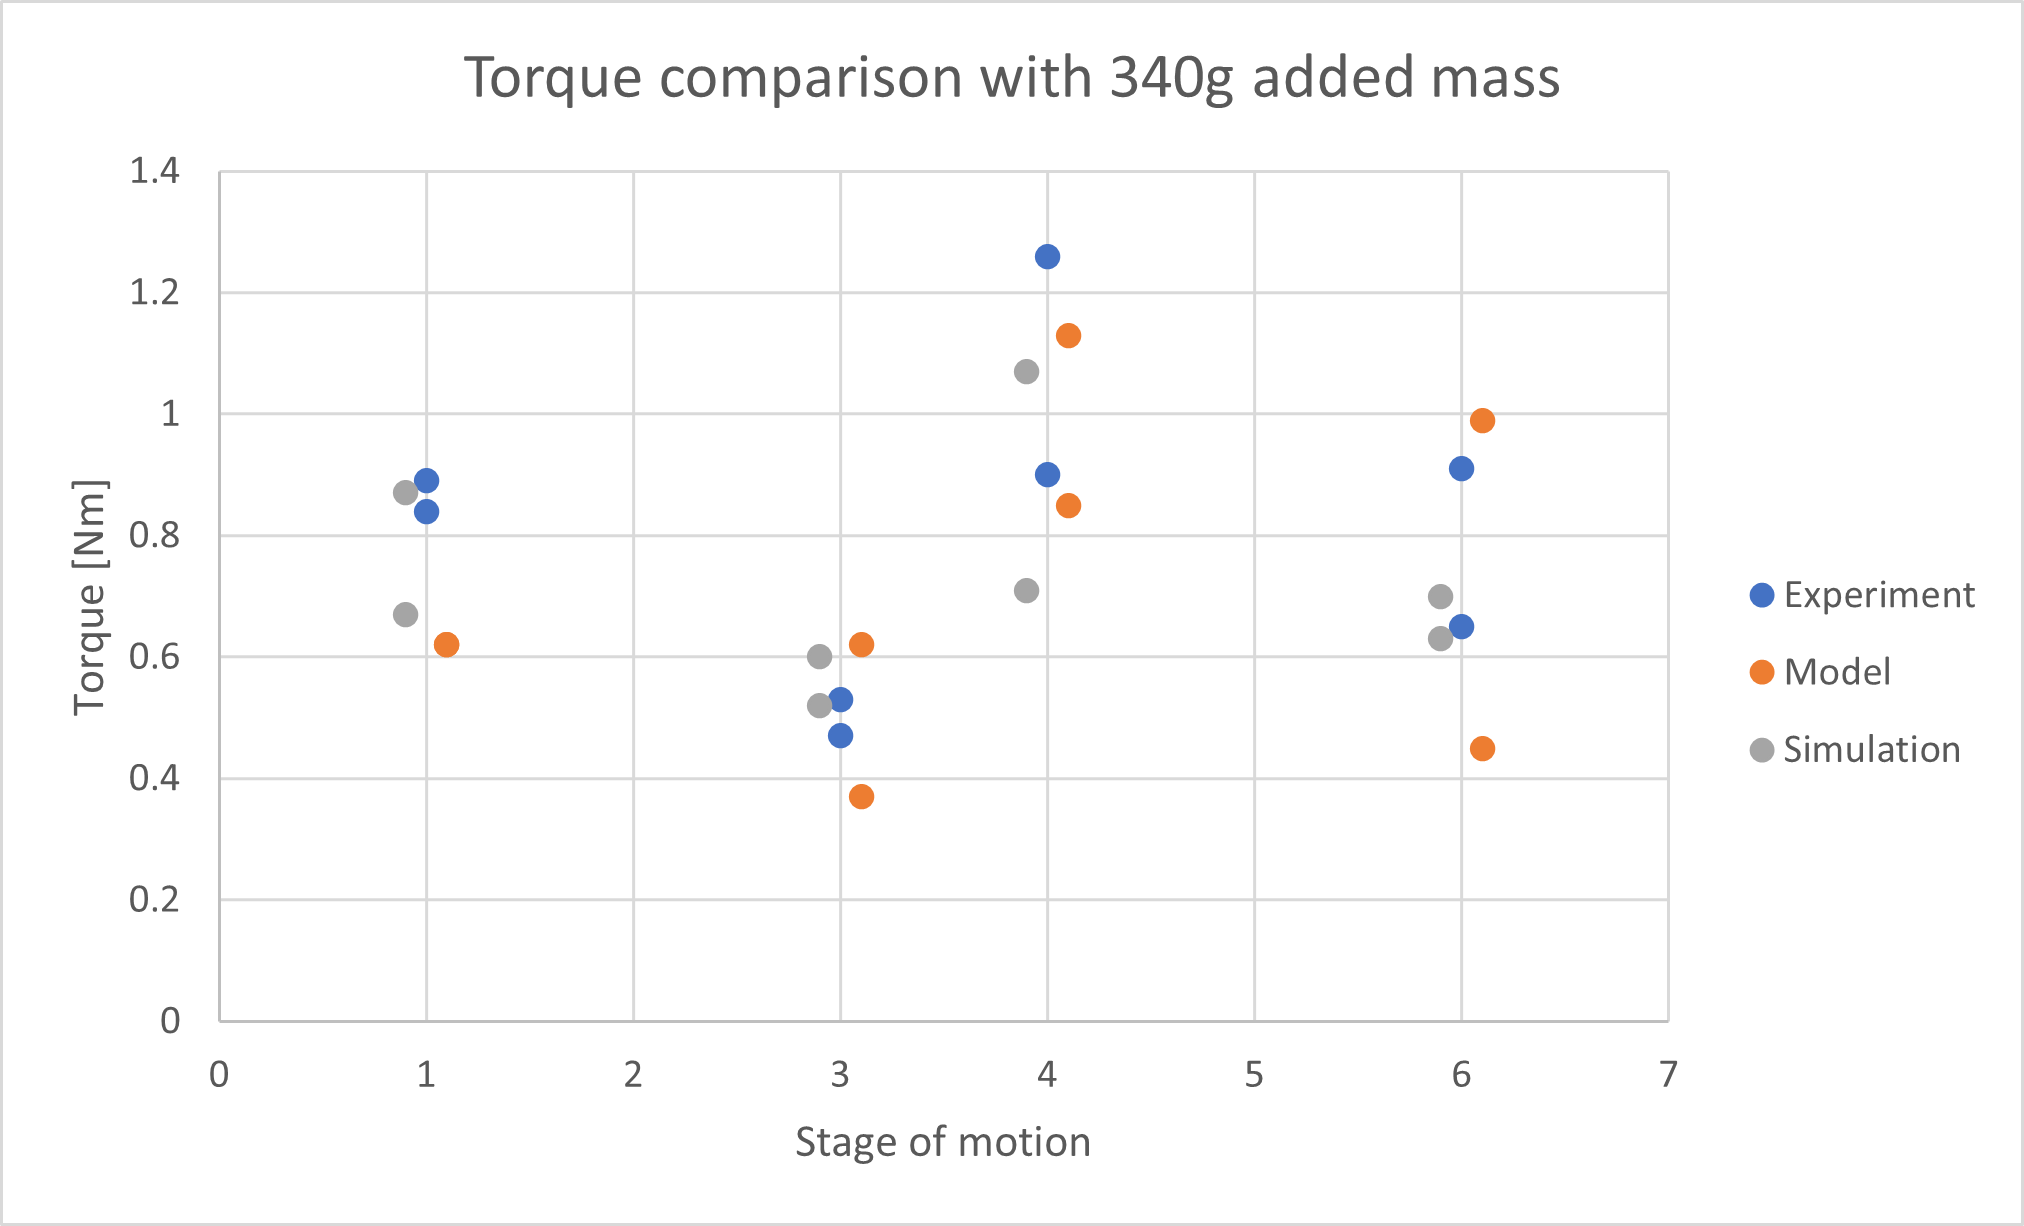
\includegraphics[width=.9\linewidth]{plots/torque-comparison-mass}
		\caption{Required torques for each stage when \\device has an added 340 g mass.}
		\label{fig:torque-comparison-mass}
	\end{subfigure}
	\caption{Required torques for each stage from different sources, with varied design parameters.}
	\label{fig:torque-comparison-tailMass}
\end{figure}


 
\section{Assessment of error}

Table \ref{tab:error} shows the percentage error of the required torque produced by the model and simulation for the original device. Negative error indicates that the model or simulation produced a lower torque value than the experiment required. The simulation is shown to be more accurate than the maths model for most data points.\\

 

\begin{table}[!ht]
	\centering
	\caption{Percentage error of required torque for each stage of motion in the model and simulation.}
	\label{tab:error}
	\begin{tabular}{|l|l|l|l|l|l|l|l|l|}
		\hline
		~ & Stage 1 & ~ & Stage 3 & ~ & Stage 4 & ~ & Stage 6 & ~ \\ \hline
		~ & Partial & Full & Partial & Full & Partial & Full & Partial & Full \\ \hline
		Model & -16.1\% & -28.8\% & -20.5\% & 33.3\% & -14.1\% & -13.5\% & -43.5\% & -11.5\% \\ \hline
		Simulation & -14.5\% & -6.8\% & 5.1\% & 23.1\% & -30.8\% & -5.6\% & -24.2\% & -24.4\% \\ \hline
	\end{tabular}
\end{table}

The full torque required to complete Stage 4 motion is the most important to design around, as this is shown to be the highest torque the device will need. In this stage, the maths model has an error of -14.1\% and the simulation has an error of -5.6\%, which indicates that one should design for at least 16.4\% higher torque than the models suggest. However, other stages of motion show errors of up to 43.5\%, which is very high and indicates that there may be some incorrect assumptions in the models.\\

Identifying the source of the error is not essential for the purposes of informing design, one can simply design the motors to have at least 2 times the calculated required torque. However, analysing the source of this error is important in order to improve future versions of the model.\\

\begin{wrapfigure}{r}{0.35\textwidth}
	\centering
	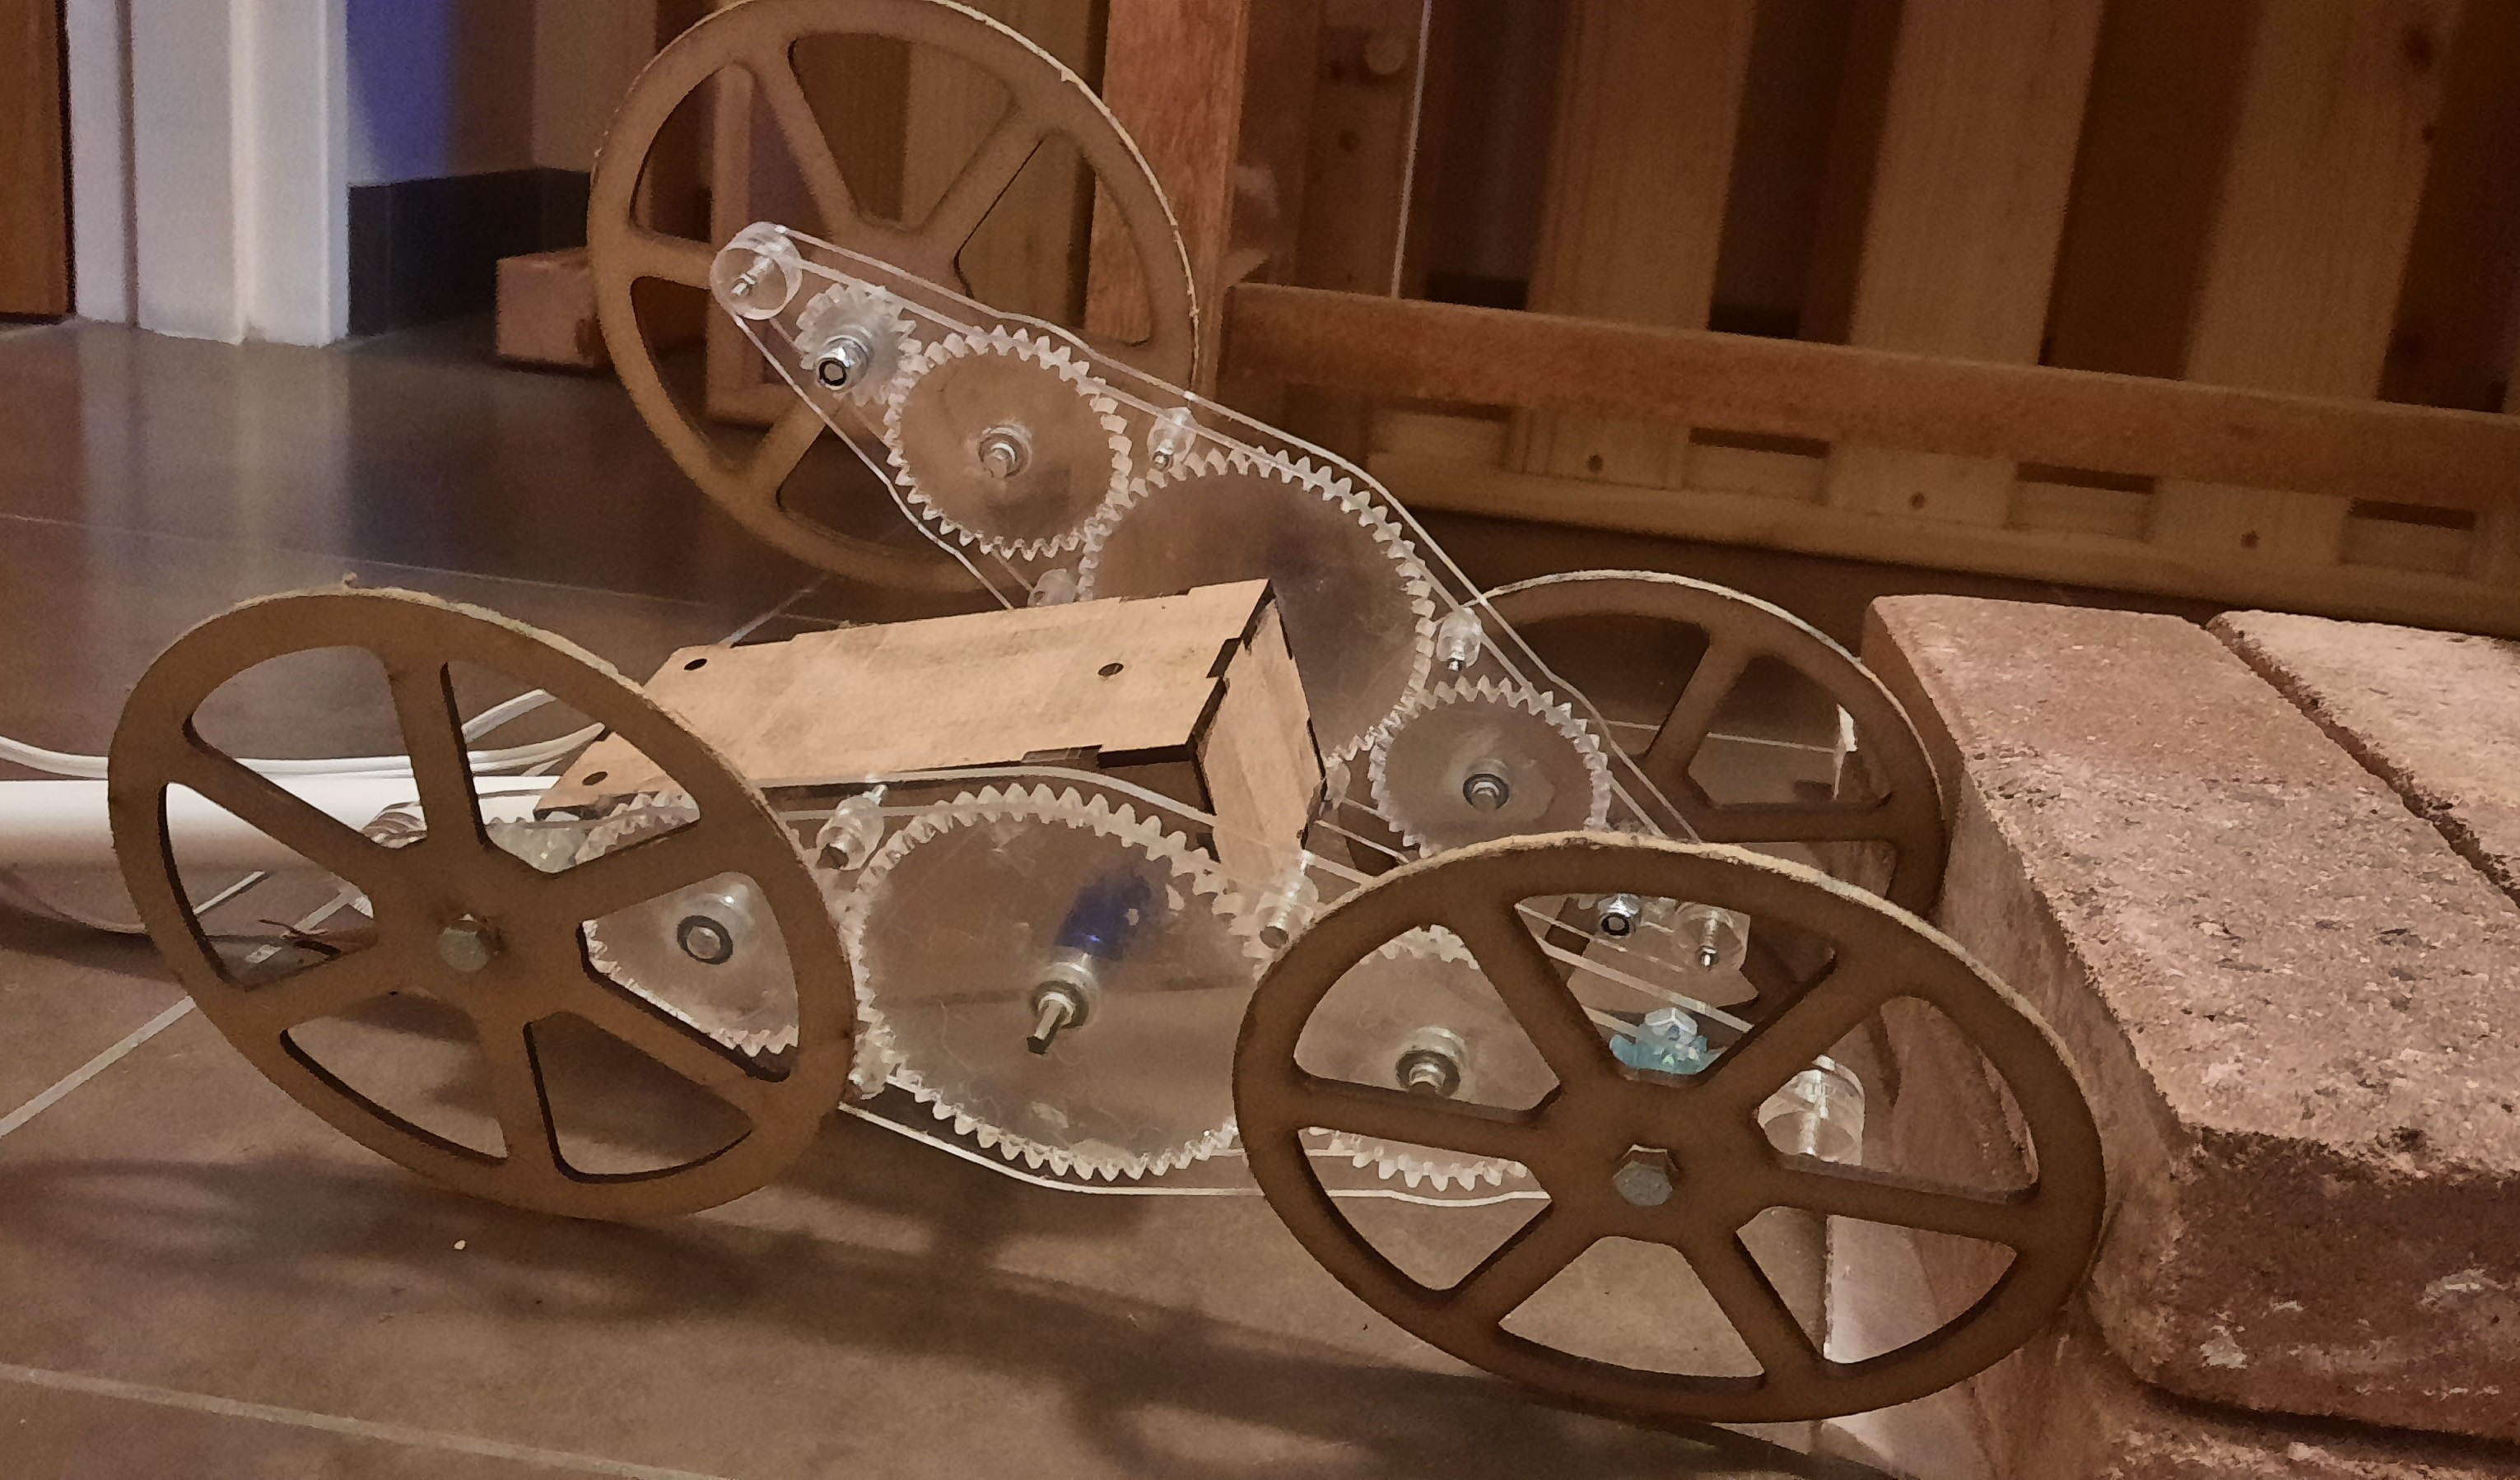
\includegraphics[width=0.35\textwidth]{imbalanced-climbing}
	\caption{Device failing to climb as one LIM lifts ahead of the other}
	\label{fig:imbalanced-climbing}
\end{wrapfigure}

In Stage 1, the model predicts that there is no torque that will cause partial movement. As the device lifts the torque required decreases, so if the torque is high enough to start lifting, it is high enough to complete Stage 1 motion. However, Figure \ref{fig:torque-comparison} shows that there is a range of torques that produce partial motion in the experimental and simulated data. The most likely cause for this is that some assumption made in the maths model is invalid. Although the calculations are done differently, the simulation is subject to the same rigid body and friction assumptions as the maths model. The main discrepancy between the two is that the simulation allows motion in three dimensions while the model is limited to two. As there is a large difference between the results of the model and the simulation, it is likely that the three-dimensional movement is what allows the device to get stuck part way during Stage 1. Initial tests showed that if one of the LIMs moves ahead of the other, the device will tip slightly, putting more weight on the LIM that falls behind, preventing the LIM from lifting unless it has excessive torque. An example of this is shown in Figure \ref{fig:imbalanced-climbing}. It is likely that even when the LIMs appear to move in unison, a slight imbalance can cause the motion to stop part way when the motor torque is close to the required torque. To address this error, one could update the maths model to allow movement in three dimensions, however this would drastically increase the complexity and the calculation time of the model, and is excessive when tools for three-dimensional simulation such as Drake are readily available.\\
\clearpage
\begin{wrapfigure}{r}{0.35\textwidth}
	\centering
	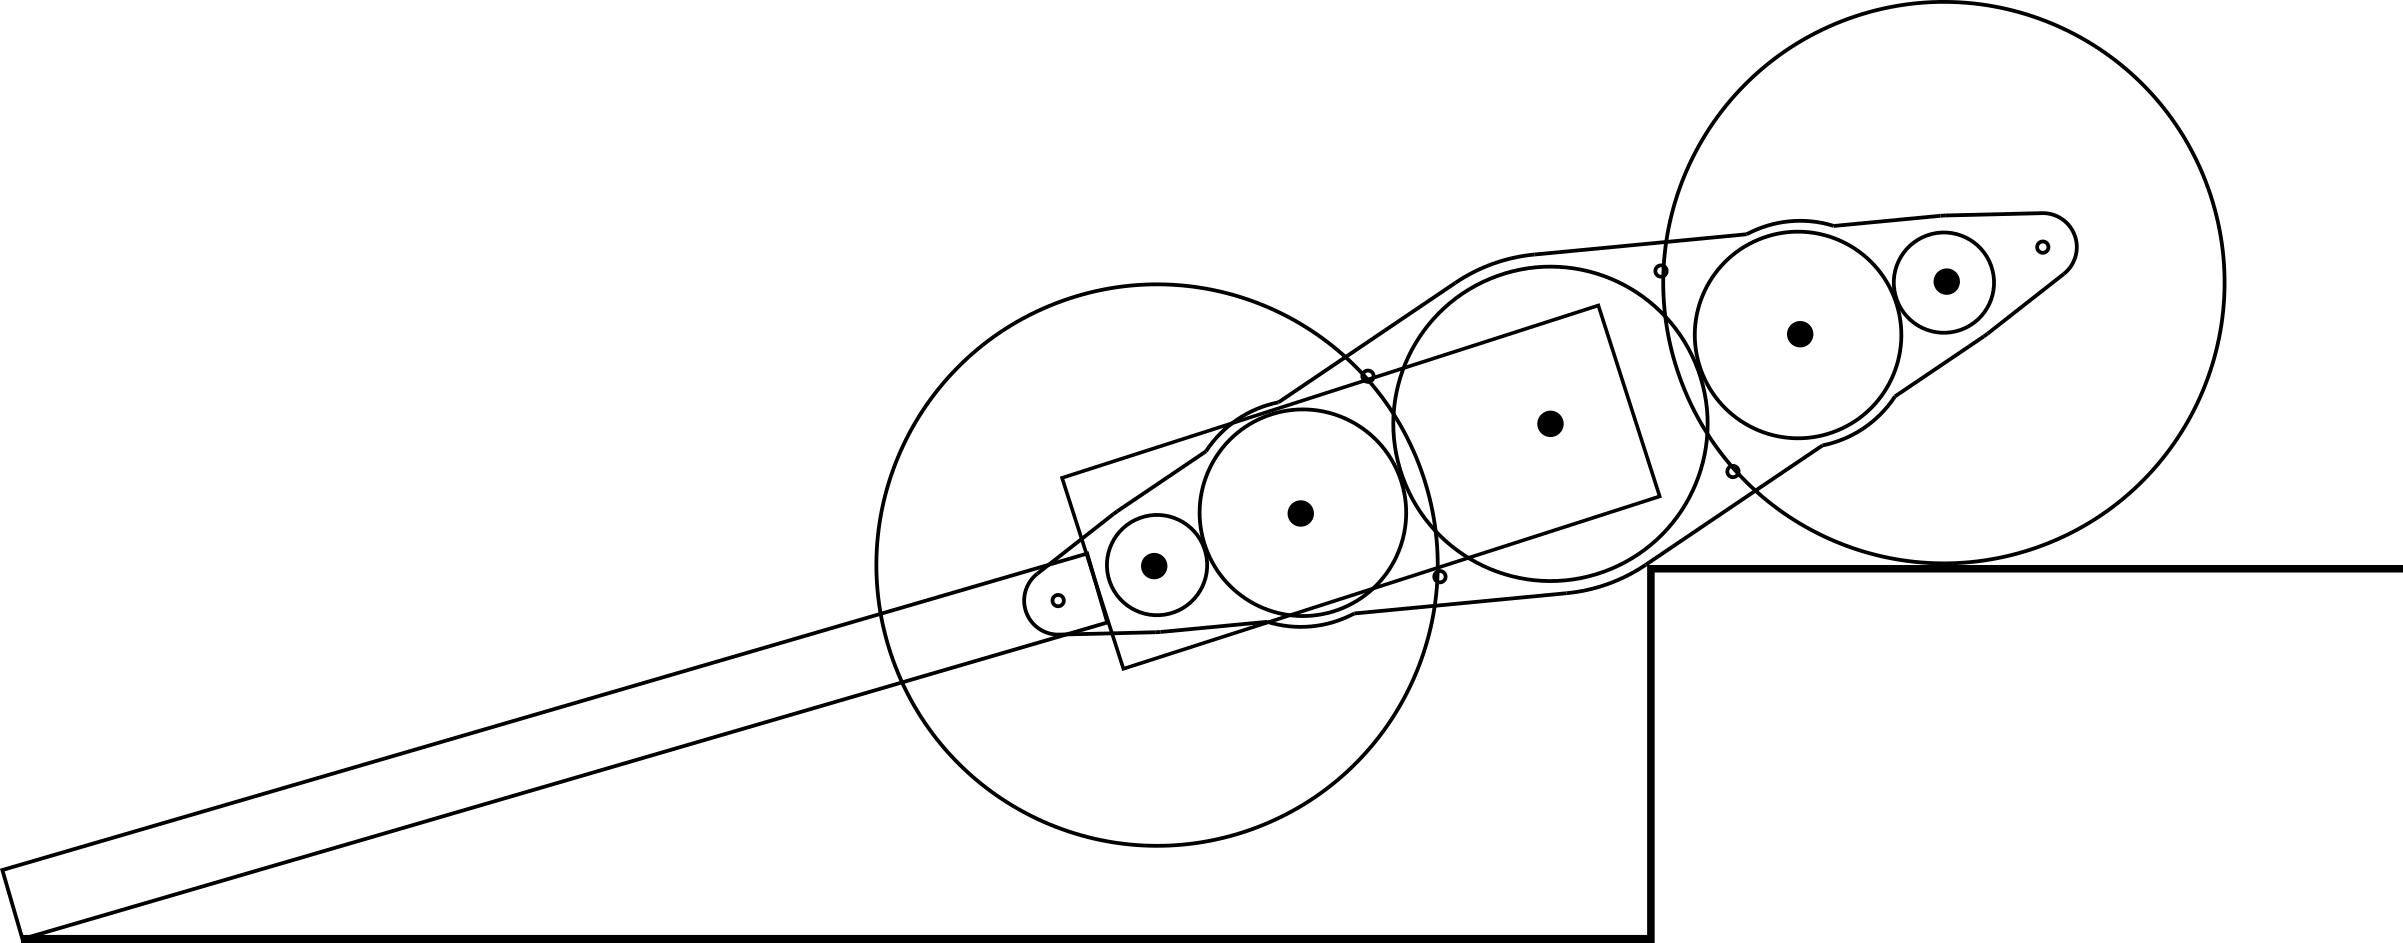
\includegraphics[width=0.35\textwidth]{FBDs/Stage-3-LIM-contact}
	\caption{Frame of the LIM making contact with the edge of the step in Stage 3}
	\label{fig:Stage-3-LIM-contact}
\end{wrapfigure}
In Stage 3, the experiment shows that there is no torque that causes partial motion. However, the simulation indicates that there is a small range of torques that cause partial motion, and the maths model indicates that there is a large range of torques that cause partial motion. Both the simulation and the maths model also indicate that the required torque is higher than the experimental value. The reason for this error in the maths model is likely because it incorrectly assumes that the frame of the LIM will not come into contact with the step. When the device climbs in Stage 3, the frame of the LIM slides along the edge of the step while the front wheel pulls the device up the step, which is illustrated in Figure \ref{fig:Stage-3-LIM-contact}.
The step supports the frame of the LIM, so that the device needs less torque in order to overcome gravity, which explains why the actual device needs less torque to complete the stage of motion than the model predicted. Interestingly, the frame does not typically make contact with the step in Stage 6 because the backwards force from the tail on the step makes the LIMs favour lifting the rear wheel instead of rolling forward. To address this error, the model could be updated to model the contact between the step and the LIM frame, however this would be difficult to do analytically as the LIM frame has an irregular shape. \\
The simulation does model the contact between the LIM frame and the step, however it still indicates that there should be partial movement and that the required torque is higher than the experimental value. Initially it was though that this was because the coefficient of friction between the LIM frame and the step is higher in the simulation than in reality, as it defaults to 1.0. However, inspection of the simulation revealed that in Stage 3 the front wheel simply does not roll forward when the motor torque is low. The LIMs will rotate, lifting the back wheel, but the front wheel does not rotate forward so the frame of the LIM is never supported by the step. This may be because the teeth of the simulated gears do not mesh well and become stuck when the torque is not high enough. As stated in Section \ref{sec:construction}, the real gears had to be filed down in order to mesh well. This indicates that there may be a flaw in the design of the gears.\\

Another potential source of error comes from the calibration of the motors. The voltage torque calibration experiment in Section \ref{sec:Voltage-torque calibration} was used to produce Equation \ref{eqTorqueVoltage}, which was later used to calculate the experimental required torque from the measured voltage. An error in the calibration method could cause all of the experimental results to be off by a constant factor. The method of this experiment involved using the motors to lift a weight with a lever. Typically in this style of experiment, the motor torque would reach an equilibrium with the moment from the weight and the lever would stop moving. However, as the gearbox on the motors is self-locking, the lever cannot move in reverse. This means that if the lever ever lifts beyond the equilibrium point, it will not fall back to the equilibrium point and the recorded lever angle will be higher than the motors could actually output. There are two possible ways that the lever can lift beyond the equilibrium point in this experiment. Firstly, if the lever and the mass have a significant momentum when they reach the equilibrium point, they will move beyond it; this is mitigated by the high gear ratio on the motor which causes it to move quite slowly. Secondly, as the mass is attached to the lever by string, it can act as a pendulum. The swing of the pendulum will sometimes make it easier for the lever to lift, and sometimes make it harder. This combines with the self-locking gearbox to cause the lever to inch forward while the pendulum is helping it, then the gearbox locks when the pendulum swings the other way. This is visualised in Figure \ref{fig:lever-swinging}. The net result is that the lever moves slightly beyond the equilibrium point. \\

\begin{figure}[!h]
	\centering
	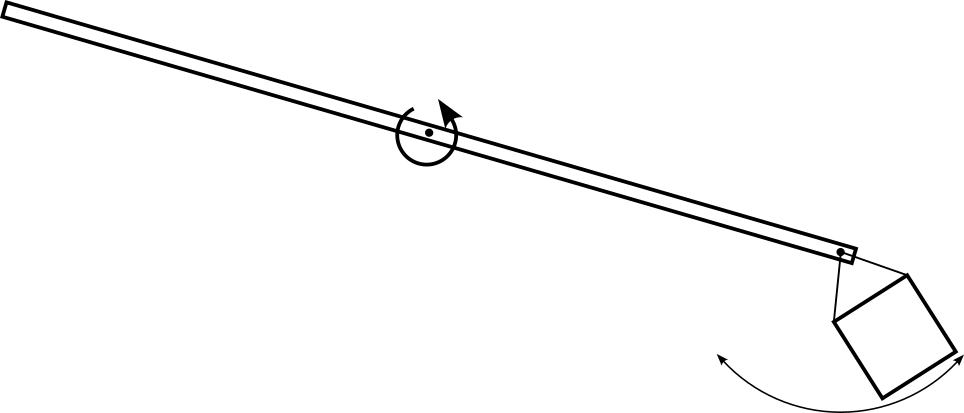
\includegraphics[width=0.6\textwidth]{FBDs/lever-swinging}
	\caption{Visualisation of the mass acting as a pendulum on the end of the lever.}
	\label{fig:lever-swinging}
\end{figure}

If the motors are imperfectly calibrated and appear to produce more torque than they actually do, it would help explain why the experimental torques are higher than the modelled and simulated torques in Stages 1, 3 and 6. This error could be reduced by attaching the mass directly to the lever rather than by string ,however there will always be some degree of error when comparing a theoretical model to the real world.


\chapter{Recommendations for future work}

This project was successful in building a LIMed device that can climb stairs. However, the device does have some limitations. It cannot turn easily, and it relies on an external power source. The logical next steps in the development of LIM robots would be to find a way to improve the turning ability of the device, and to design a device that can be operated remotely. 


\section{Recommendation for design}

When designing a device that uses LIMs, this project recommends first using the maths model to inform the selection design parameters. This can be done by changing a parameter and noting how it affects the performance of the design, similar to what was done in Figure \ref{fig:GR-friction}. Once the design parameters have been selected, the device should be designed in CAD and converted to SDFormat. From there the device can be simulated using Drake, and if performance is satisfactory it can be built. Instructions on how to perform each of these steps can be found in the project folder ???.\\

\chapter{Conclusions}

This report details the design, modelling, and model validation of a novel gearing system for robot locomotion. The advantage of this LIM gearing system is that it allows a device to roll forward or climb steps using a single actuator, reducing costs, while also being able to fit into low voids. The model produced by this report could be used to inform the design of future USAR robots. This project builds and improves upon previous work, and produces the first LIM robot capable of climbing steps consistently and sequentially. \\

To explore the motion of the LIMS, a preliminary two-dimensional simulation was performed, and the stair climbing motion of the device was categorised into six distinct stages. This project proposes a mathematical model to describe the motion a LIMed device, using the MATLAB symbolic toolbox. The maths model consists of a large set of simultaneous equations that are solved simultaneously, and this report presents an algorithm that uses the MATLAB functions to efficiently solve this large set of equations. Additionally, this project explores the use of Drake, a multi-body simulator, to model the device. \\

Both the maths model and simulation are validated against real world data. The validation showed that the torque required to climb stairs sequentially was 16.4\% higher than the maths model predicted, and 5.9\% higher than the simulation predicted. This report explores the reasons for this error, which are attributed to incorrect assumptions and calibration methods.\\

In conclusion, this project was successful in completing its objectives. Both the model and simulation have been validated and their error has been quantified, they can be used to inform future work on LIMed robots.

%\chapter{Design- 1st iteration}

Starting with Powrie's device as it is the most developed of the previous projects.\\
Attempted to use mathematical model to identify potential improvements, however I struggled to get objective improvements, increasing one parameter often may improve the ability to flip but hinder the ability to climb overall, and removing material should only be done if it has minimal effect on structure strength, something that would take much time to determine (possibly with FEM?). Such optimisations are beyond the scope of the project, I'm not trying to create a perfectly optimised device, I'm trying to create a working device so I can describe its function. Powrie’s device is working to some extent, so the first design iteration should deviate minimally from his design.\\
Powrie's design for the LIMs is copied as accurately as possible, could possibly even use his laser cutting templates to manufacture. Fortunately he provides a detailed builder's guide, allowing me to design and build ASAP so I can focus on the math model. The robot body is changed significantly. Powrie uses external gears on an already geared motor, this is unnecessary, as geared motors come in a variety of ratios. I use a JGY-370 motor, as I believe the worm gearbox is well suited to this purpose, it allows me to make a thinner body that doesn't protrude as far forward beyond the axle. The tail is designed based on Powrie’s concepts. The motors selected produce more torque than the ones Powrie selected, even with his additional gearing, so they should be up to the task. Later iterations could combine the worm gearbox with even more powerful brushless motors.
%\chapter{Description of motion}

The device can climb up steps. In doing so, the wheels and tail make contact with different parts of the steps. In order to model the device, the overall movement is broken down into individual sequential motions.\\
The first motion is simple, the device rolls forward on a flat surface.\\
The second motion is referred to as climbing. The front wheel is blocked by a step and fixed in place. The tail pushes against the ground and the LIM starts rotating up the step. This motion ends when the LIM is vertical.\\
In the third motion, the top wheel falls forward onto the step and the bottom wheel rolls backwards until the top wheel lands. The distance that it rolls depends on the speed of the LIM and the height of the step. If the frame of the LIM hits the edge of the step, the device may slip backwards until the top wheel makes contact with the step. This motion ends when the top wheel is on the step.\\
In the fourth motion, the device pulls itself up the steps. The front wheel rests on the step while the back wheel is on the ground. The tail pushes against the ground and the bottom wheel lifts while the front wheel simultaneously rolls forward on the step. This motion ends when the top wheel reaches the next step.\\
The fifth motion is similar to the second motion, with the exception that the tail is angled further down to reach the ground.\\
The sixth motion is similar to the third motion, with the exception that the tail is angled further down to reach the ground.\\
The seventh motion deviates significantly from the previous motions. The front wheel starts on the next step while the bottom wheel starts on the previous step. The tail now contacts the edge of the previous step rather than the ground, which causes a significant force to pull the LIMs backwards. Because of this, unlike in the fourth motion, the front wheel will not initially roll forward on the next step. The back wheel will lift from below until it is at a certain angle above the front wheel, at which point the front wheel will start to roll forward, bringing it to the base of the next step.\\
The eighth motion is similar to the second motion, except the tail pushes against the edge of the previous step and the back wheel is already partially lifted. The back wheel then lifts up further until the LIM is vertical.\\
The ninth motion is similar to the sixth motion, except the tail pushes against the surface of the previous step instead of the ground.


%\chapter{Conclusions}

This report details the design, modelling, and model validation of a novel gearing system for robot locomotion. The advantage of this LIM gearing system is that it allows a device to roll forward or climb steps using a single actuator, reducing costs, while also being able to fit into low voids. The model produced by this report could be used to inform the design of future USAR robots. This project builds and improves upon previous work, and produces the first LIM robot capable of climbing steps consistently and sequentially. \\

To explore the motion of the LIMS, a preliminary two-dimensional simulation was performed, and the stair climbing motion of the device was categorised into six distinct stages. This project proposes a mathematical model to describe the motion a LIMed device, using the MATLAB symbolic toolbox. The maths model consists of a large set of simultaneous equations that are solved simultaneously, and this report presents an algorithm that uses the MATLAB functions to efficiently solve this large set of equations. Additionally, this project explores the use of Drake, a multi-body simulator, to model the device. \\

Both the maths model and simulation are validated against real world data. The validation showed that the torque required to climb stairs sequentially was 16.4\% higher than the maths model predicted, and 5.9\% higher than the simulation predicted. This report explores the reasons for this error, which are attributed to incorrect assumptions and calibration methods.\\

In conclusion, this project was successful in completing its objectives. Both the model and simulation have been validated and their error has been quantified, they can be used to inform future work on LIMed robots.

\appendix%------------------------------------------------------------
\titleformat{\chapter}[hang] 
{\normalfont\huge\bfseries}{\chaptertitlename\ \thechapter}{1em}{} 


\chapter{ECSA Outcome Self Assessment}

\begin{table}[h]
	\caption{ECSA outcome self assessment}
	\footnotesize
	\begin{tabular}{ | p{22em} | p{17em} |} 
		\hline
		ECSA outcome& Application \\ 
		\hline
		Demonstrate competence to identify, assess, formulate and solve convergent and
		divergent engineering problems creatively and innovatively. & 
		The design aspect of this project required creative solutions to overcome the limitations of previous designs. \\ 
		\hline
		Application of scientific and engineering knowledge: Demonstrate competence to apply knowledge
		of mathematics, basic science and engineering sciences from first principles to solve engineering problems. & 
		Producing the mathematical model required building a set of equations from first principles. \\ 
		\hline
		Engineering Design: Demonstrate competence to perform creative, procedural and non-procedural design and synthesis of components, systems, engineering works, products or processes.& This project designs a device, a model, a simulation pipeline, and an experiment. \\ 
		\hline
		Engineering methods, skills and tools, including Information Technology: Demonstrate competence
		to use appropriate engineering methods, skills and tools, including those based on information technology. & 
		The project involves designing a device using CAD, a controller in C, a math model in MATLAB, and a simulation pipeline using python.\\ 
		\hline
		Professional and technical communication: Demonstrate competence to communicate effectively,
		both orally and in writing, with engineering audiences and the community at large. & 
		All deliverables, including the proposal, progress report, final report, and presentation will demonstrate competent and effective communication. \\ 
		\hline
		Individual, Team and Multidisciplinary Working: Demonstrate competence to work effectively as an
		individual, in teams and in multi-disciplinary environments. & 
		This project is done individually, with input from the project supervisor and stakeholder. \\ 
		\hline
		Independent Learning Ability: Demonstrate competence to engage in independent learning through
		well-developed learning skills. & 
		Research is done in the literature review, and the use of tools such as Drake required independent learning. \\ 
		\hline
	\end{tabular}
\end{table}
\chapter{Techno-economic analysis}

This appendix contains an approximate budget and Gantt chart for the planned activities.

\begin{table}[h!]
	\centering
	\begin{tabular}{ | m{15em} | m{3em} | m{3em} |m{4em} | m{4em} | m{4em}| } 
		\hline
		Activity & \multicolumn{2}{|c|}{Engineering time} & Running costs & Facility use & Capital costs \\ 
		\hline
		&hr & R & R & R & R\\
		\hline
		Review Literature &25&11250&250&&\\
		\hline
		Compile Design Requirements&25&11250&250&&\\
		\hline
		Design localiser device&150&67500&500&500&\\
		\hline
		Produce Prototype&125&56250&1000&1500&1500\\
		\hline
		Test Prototype&50&22500&1000&500&\\
		\hline
		Finalise Report&100&45000&500&&\\
		\hline
		Total&475&213750&3500&2500&1500\\
		\hline
		Grand Total (R)&221725&&&&\\ 
		\hline
	\end{tabular}
\caption{Estimated cost per activity}
\end{table}

\noindent This budget is based on a standard rate of R450/h. The capital costs include estimates for the microphones and Analogue to digital converter.

\begin{figure}[h]
	\centering
	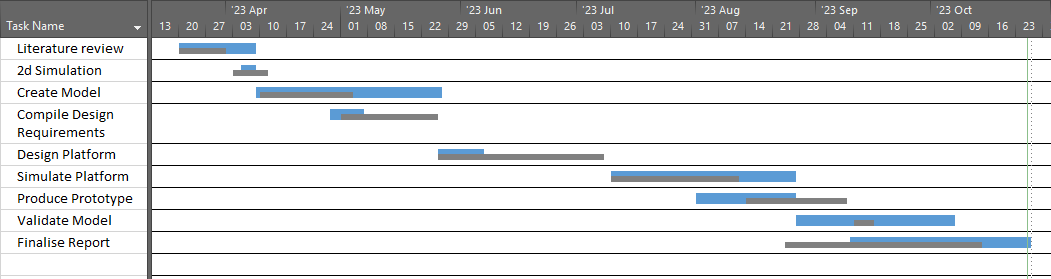
\includegraphics[width=1.5\textwidth,angle=90]{Gantt}
	\caption{Gantt Chart}
	\label{fig:mesh1}
\end{figure}
\chapter{Risk Assessment}

The device uses a maximum voltage of 12 V, which is considered safe to touch. Gears are enclosed within the frame of the LIMs, however power should still be disconnected when handling the device as the geared motors can produce significant torque. To prevent motor burnout, they should not be left stalling for more than a few seconds at a time.\\

\noindent The main risk to the feasibility of the project was that there would not be enough time to build a fully functioning robot platform. The projects preceding this one all encountered complications when building robot platforms that they were unable to solve within the time constraints of their projects. This risk was mitigated by completing activities in a timely manner as described in the Gantt. Chart, as well as careful planning and consideration of previous pitfalls.
\\

\noindent There was also the risk that it would be impossible to create a closed form model to describe the dynamics of the system. Fortunately, this was not the case.\\

\noindent There was a risk that the project would exceed the allowed cost. This is because the prototype may have required hardware such as high powered motors, custom parts, encoders, controllers, and possibly batteries, which could have a considerable cost. This was be mitigated simplifying the design to only use the minimum hardware required to build a prototype.\\


\chapter{Resource use and end of life strategy}

This project built a prototype device that has a motor, a controller, wheels, and several custom parts such as gears and frames. A battery was not included as it is unnecessary for a prototype build which can otherwise be wired to a power supply.
The device benefits from having a low mass, so there was already an incentive to use materials sparingly. Before construction, the design was be simulated to ensure that it meets requirements; this mitigated the chance that a second prototype would need to be built. Upon completion of the project, the prototype can be disassembled and the motor, controller, and wheels can be reused in future projects. The custom parts are specific to this design so will not be suitable for most reuse applications; they shall be recycled. If the materials are such that they cannot be recycled, then they shall be disposed of instead. These materials are chemically inert (not hazardous).

\chapter{Data} \label{app:data}


\begin{table}[!ht]
	\centering
	\caption{Required torque (Nm) for each stage of motion from the model, simulation, and experiment.}
	\footnotesize
	\begin{tabular}{|l|l|l|l|l|l|l|l|l|l|}
		\hline
		Stage & ~ & ~ & ~ & ~ & ~ & ~ & ~ & ~ & ~ \\ \hline
		~ & ~ & 1 & 1 & 3 & 3 & 4 & 4 & 6 & 6 \\ \hline
		~ & ~ & partial & full & partial & full & partial & full & partial & full \\ \hline
		default & Model & 0.52 & 0.52 & 0.31 & 0.52 & 0.67 & 0.77 & 0.35 & 0.69 \\ \hline
		~ & Simulation & 0.53 & 0.68 & 0.41 & 0.48 & 0.54 & 0.84 & 0.47 & 0.59 \\ \hline
		~ & Experiment & 0.62 & 0.73 & 0.39 & 0.39 & 0.78 & 0.89 & 0.62 & 0.78 \\ \hline
		60cm tail & model & 0.58 & 0.58 & 0.33 & 0.58 & 0.7 & 0.75 & 0.38 & 0.77 \\ \hline
		~ & simulation & 0.71 & 0.8 & 0.56 & 0.56 & 0.8 & 0.85 & 0.48 & 0.6 \\ \hline
		~ & experiment & 0.71 & 0.75 & 0.39 & 0.48 & 0.78 & 0.95 & 0.61 & 0.78 \\ \hline
		343g mass & model & 0.62 & 0.62 & 0.37 & 0.62 & 0.85 & 1.13 & 0.45 & 0.99 \\ \hline
		~ & simulation & 0.67 & 0.87 & 0.52 & 0.6 & 0.71 & 1.07 & 0.63 & 0.7 \\ \hline
		~ & experiment & 0.84 & 0.89 & 0.47 & 0.53 & 0.9 & 1.26 & 0.65 & 0.91 \\ \hline
	\end{tabular}
\end{table}
\begin{landscape}

\begin{table}[!ht]
	\centering
	\caption{Voltage, assessment, and calculated torque for Stage 1 motion.}
	\footnotesize
	\begin{tabular}{|l|l|l|l|l|l|l|l|l|}
		\hline
		Default device & ~ & ~ & 60 cm tail & ~ & ~ & 340g added weight & ~ & ~ \\ \hline
		Voltage (V) & Assessment & Torque (Nm) & Voltage (V) & Assessment & Torque (Nm) & Voltage (V) & Assessment & Torque (Nm) \\ \hline
		0.89 & 0 & 0.099974 & 1.58 & 0 & 0.456428 & 2.58 & 1 & 0.973028 \\ \hline
		1.08 & 0 & 0.198128 & 1.95 & 0 & 0.64757 & 2.78 & 1 & 1.076348 \\ \hline
		1.12 & 0 & 0.218792 & 2.04 & 0 & 0.694064 & 2.42 & 1 & 0.890372 \\ \hline
		1.57 & 0 & 0.451262 & 2.65 & 1 & 1.00919 & 1.99 & 0 & 0.668234 \\ \hline
		1.68 & 0 & 0.508088 & 2.41 & 1 & 0.885206 & 1.77 & 0 & 0.554582 \\ \hline
		1.74 & 0 & 0.539084 & 2.24 & 1 & 0.797384 & 2.06 & 0 & 0.704396 \\ \hline
		1.81 & 0 & 0.575246 & 2.16 & 1 & 0.756056 & 2.15 & 0 & 0.75089 \\ \hline
		1.87 & 0 & 0.606242 & 2.08 & 0.5 & 0.714728 & 2.2 & 0 & 0.77672 \\ \hline
		1.89 & 0.5 & 0.616574 & 2.03 & 0 & 0.688898 & 2.44 & 1 & 0.900704 \\ \hline
		1.98 & 0.5 & 0.663068 & 2.09 & 0.5 & 0.719894 & 2.31 & 0.5 & 0.833546 \\ \hline
		2.05 & 0.5 & 0.69923 & 2.14 & 0.5 & 0.745724 & 2.32 & 0.5 & 0.838712 \\ \hline
		2.11 & 1 & 0.730226 & 2.28 & 1 & 0.818048 & 2.49 & 1 & 0.926534 \\ \hline
		2.13 & 1 & 0.740558 & ~ & ~ & ~ & ~ & ~ & ~ \\ \hline
		2.25 & 1 & 0.80255 & ~ & ~ & ~ & ~ & ~ & ~ \\ \hline
		2.26 & 1 & 0.807716 & ~ & ~ & ~ & ~ & ~ & ~ \\ \hline
		2.3 & 1 & 0.82838   & ~ & ~ & ~ & ~ & ~ & ~ \\ \hline
	\end{tabular}
\end{table}

\begin{table}[!ht]
	\centering
	\caption{Voltage, assessment, and calculated torque for Stage 3 motion.}
	\footnotesize
	\begin{tabular}{|l|l|l|l|l|l|l|l|l|}
		\hline
		Default device & ~ & ~ & 60 cm tail & ~ & ~ & 340g added weight & ~ & ~ \\ \hline
		Voltage (V) & Assessment & Torque (Nm) & Voltage (V) & Assessment & Torque (Nm) & Voltage (V) & Assessment & Torque (Nm) \\ \hline
		2.25 & 1 & 0.80255 & 2.65 & 1 & 1.00919 & 2.35 & 1 & 0.85421 \\ \hline
		1.73 & 1 & 0.533918 & 2.56 & 1 & 0.962696 & 2.3 & 1 & 0.82838 \\ \hline
		1.45 & 1 & 0.38927 & 2.06 & 1 & 0.704396 & 2.03 & 1 & 0.688898 \\ \hline
		1.49 & 1 & 0.409934 & 1.61 & 1 & 0.471926 & 1.75 & 1 & 0.54425 \\ \hline
		0.66 & 0 & -0.018844 & 1.45 & 0.5 & 0.38927 & 1.64 & 0.5 & 0.487424 \\ \hline
		0.81 & 0 & 0.058646 & 1.22 & 0 & 0.270452 & 1.69 & 0.5 & 0.513254 \\ \hline
		0.99 & 0 & 0.151634 & 1.06 & 0 & 0.187796 & 1.73 & 1 & 0.533918 \\ \hline
		1.07 & 0 & 0.192962 & 1.39 & 0 & 0.358274 & 1.5 & 0 & 0.4151 \\ \hline
		1.25 & 0 & 0.28595 & 1.42 & 0 & 0.373772 & 1.41 & 0 & 0.368606 \\ \hline
		1.3 & 0 & 0.31178 & 1.45 & 0 & 0.38927 & 1.56 & 0 & 0.446096 \\ \hline
		1.34 & 0 & 0.332444 & 1.41 & 0 & 0.368606 & 1.58 & 0 & 0.456428 \\ \hline
		1.42 & 0 & 0.373772 & 1.52 & 0.5 & 0.425432 & 1.61 & 0.5 & 0.471926 \\ \hline
		1.49 & 1 & 0.409934 & 1.63 & 1 & 0.482258 & ~ & ~ & ~ \\ \hline
		~ & ~ & ~ & 1.72 & 1 & 0.528752 & ~ & ~ & ~ \\ \hline
		~ & ~ & ~ & 1.67 & 1 & 0.502922 & ~ & ~ & ~ \\ \hline
		~ & ~ & ~ & 1.49 & 0 & 0.409934 & ~ & ~ & ~ \\ \hline
		~ & ~ & ~ & 1.56 & 0.5 & 0.446096 & ~ & ~ & ~ \\ \hline
	\end{tabular}
\end{table}

\begin{table}[!ht]
	\centering
	\caption{Voltage, assessment, and calculated torque for Stage 4 motion.}
	\footnotesize
	\begin{tabular}{|l|l|l|l|l|l|l|l|l|}
		\hline
		Default device & ~ & ~ & 60 cm tail & ~ & ~ & 340g added weight & ~ & ~ \\ \hline
		Voltage (V) & Assessment & Torque (Nm) & Voltage (V) & Assessment & Torque (Nm) & Voltage (V) & Assessment & Torque (Nm) \\ \hline
		2.61 & 1 & 0.988526 & 1.68 & 0 & 0.508088 & 1.58 & 0 & 0.456428 \\ \hline
		2.91 & 1 & 1.143506 & 2.81 & 1 & 1.091846 & 1.84 & 0 & 0.590744 \\ \hline
		2.99 & 1 & 1.184834 & 2.79 & 1 & 1.081514 & 2.07 & 0 & 0.709562 \\ \hline
		2.83 & 1 & 1.102178 & 2.42 & 0.5 & 0.890372 & 2.38 & 0 & 0.869708 \\ \hline
		2.78 & 1 & 1.076348 & 2.21 & 0 & 0.781886 & 2.66 & 0.5 & 1.014356 \\ \hline
		2.65 & 1 & 1.00919 & 2.04 & 0 & 0.694064 & 2.61 & 0.5 & 0.988526 \\ \hline
		2.56 & 1 & 0.962696 & 1.73 & 0 & 0.533918 & 2.48 & 0.5 & 0.921368 \\ \hline
		2.48 & 1 & 0.921368 & 1.93 & 0 & 0.637238 & 2.47 & 0.5 & 0.916202 \\ \hline
		2.43 & 1 & 0.895538 & 2.26 & 0.5 & 0.807716 & 2.45 & 0.5 & 0.90587 \\ \hline
		2.28 & 0.5 & 0.818048 & 2.32 & 0.5 & 0.838712 & 2.42 & 0.5 & 0.890372 \\ \hline
		2.38 & 0.5 & 0.869708 & 2.15 & 0 & 0.75089 & 2.2 & 0 & 0.77672 \\ \hline
		2.3 & 0.5 & 0.82838 & 2.22 & 0 & 0.787052 & 2.27 & 0 & 0.812882 \\ \hline
		2.22 & 0.5 & 0.787052 & 2.36 & 0.5 & 0.859376 & 2.43 & 0.5 & 0.895538 \\ \hline
		2.08 & 0 & 0.714728 & 2.62 & 1 & 0.993692 & 2.66 & 0.5 & 1.014356 \\ \hline
		2 & 0 & 0.6734 & 2.63 & 1 & 0.998858 & 2.93 & 0.5 & 1.153838 \\ \hline
		2.12 & 0 & 0.735392 & 2.53 & 1 & 0.947198 & 3.18 & 1 & 1.282988 \\ \hline
		2.16 & 0 & 0.756056 & 2.25 & 0.5 & 0.80255 & 3.04 & 0.5 & 1.210664 \\ \hline
		~ & ~ & ~ & 2.22 & 0.5 & 0.787052 & 3.1 & 0.5 & 1.24166 \\ \hline
		~ & ~ & ~ & 2.6 & 1 & 0.98336 & 3.34 & 1 & 1.365644 \\ \hline
		~ & ~ & ~ & ~ & ~ & ~ & 3.14 & 1 & 1.262324 \\ \hline
	\end{tabular}
\end{table}

\begin{table}[!ht]
	\centering
	\caption{Voltage, assessment, and calculated torque for Stage 6 motion.}
	\footnotesize
	\begin{tabular}{|l|l|l|l|l|l|l|l|l|}
		\hline
		Default device & ~ & ~ & 60 cm tail & ~ & ~ & 340g added weight & ~ & ~ \\ \hline
		Voltage (V) & Assessment & Torque (Nm) & Voltage (V) & Assessment & Torque (Nm) & Voltage (V) & Assessment & Torque (Nm) \\ \hline
		1.52 & 0 & 0.425432 & 1.91 & 0.5 & 0.626906 & 3.42 & 1 & 1.406972 \\ \hline
		1.68 & 0 & 0.508088 & 1.78 & 0 & 0.559748 & 2.81 & 1 & 1.091846 \\ \hline
		1.91 & 0.5 & 0.626906 & 1.83 & 0 & 0.585578 & 2.05 & 0.5 & 0.69923 \\ \hline
		2.12 & 0.5 & 0.735392 & 1.87 & 0.5 & 0.606242 & 2.09 & 0.5 & 0.719894 \\ \hline
		2.45 & 1 & 0.90587 & 1.95 & 0.5 & 0.64757 & 2.15 & 0.5 & 0.75089 \\ \hline
		2.22 & 1 & 0.787052 & 2.13 & 0.5 & 0.740558 & 2.12 & 0.5 & 0.735392 \\ \hline
		2.33 & 1 & 0.843878 & 2.27 & 1 & 0.812882 & 2.3 & 0.5 & 0.82838 \\ \hline
		2.08 & 0.5 & 0.714728 & 2.23 & 1 & 0.792218 & 2.46 & 1 & 0.911036 \\ \hline
		2.1 & 0.5 & 0.72506 & 2.2 & 1 & 0.77672 & 2.43 & 0.5 & 0.895538 \\ \hline
		2.2 & 1 & 0.77672 & 2.17 & 0.5 & 0.761222 & 2.41 & 0.5 & 0.885206 \\ \hline
		1.6 & 0 & 0.46676 & 2.23 & 1 & 0.792218 & 2.46 & 0.5 & 0.911036 \\ \hline
		1.92 & 0.5 & 0.632072 & ~ & ~ & ~ & 2.48 & 1 & 0.921368 \\ \hline
		1.84 & 0 & 0.590744 & ~ & ~ & ~ & 2.7 & 1 & 1.03502 \\ \hline
		1.91 & 0.5 & 0.626906 & ~ & ~ & ~ & 2.79 & 1 & 1.081514 \\ \hline
		~ & ~ & ~ & ~ & ~ & ~ & 2.65 & 1 & 1.00919 \\ \hline
		~ & ~ & ~ & ~ & ~ & ~ & 1.95 & 0.5 & 0.64757 \\ \hline
		~ & ~ & ~ & ~ & ~ & ~ & 1.92 & 0 & 0.632072 \\ \hline
	\end{tabular}
\end{table}

\end{landscape}
\chapter{Engineering drawings and parts list}

This appendix contains the engineering drawings of the LIM device. The .dxf files of the parts to be laser cut can be found in Drawing-files/v2/ in the project repository \citep{repo}.
%\afterpage{
%\KOMAoptions{paper=A3,paper=landscape,pagesize}
%\recalctypearea

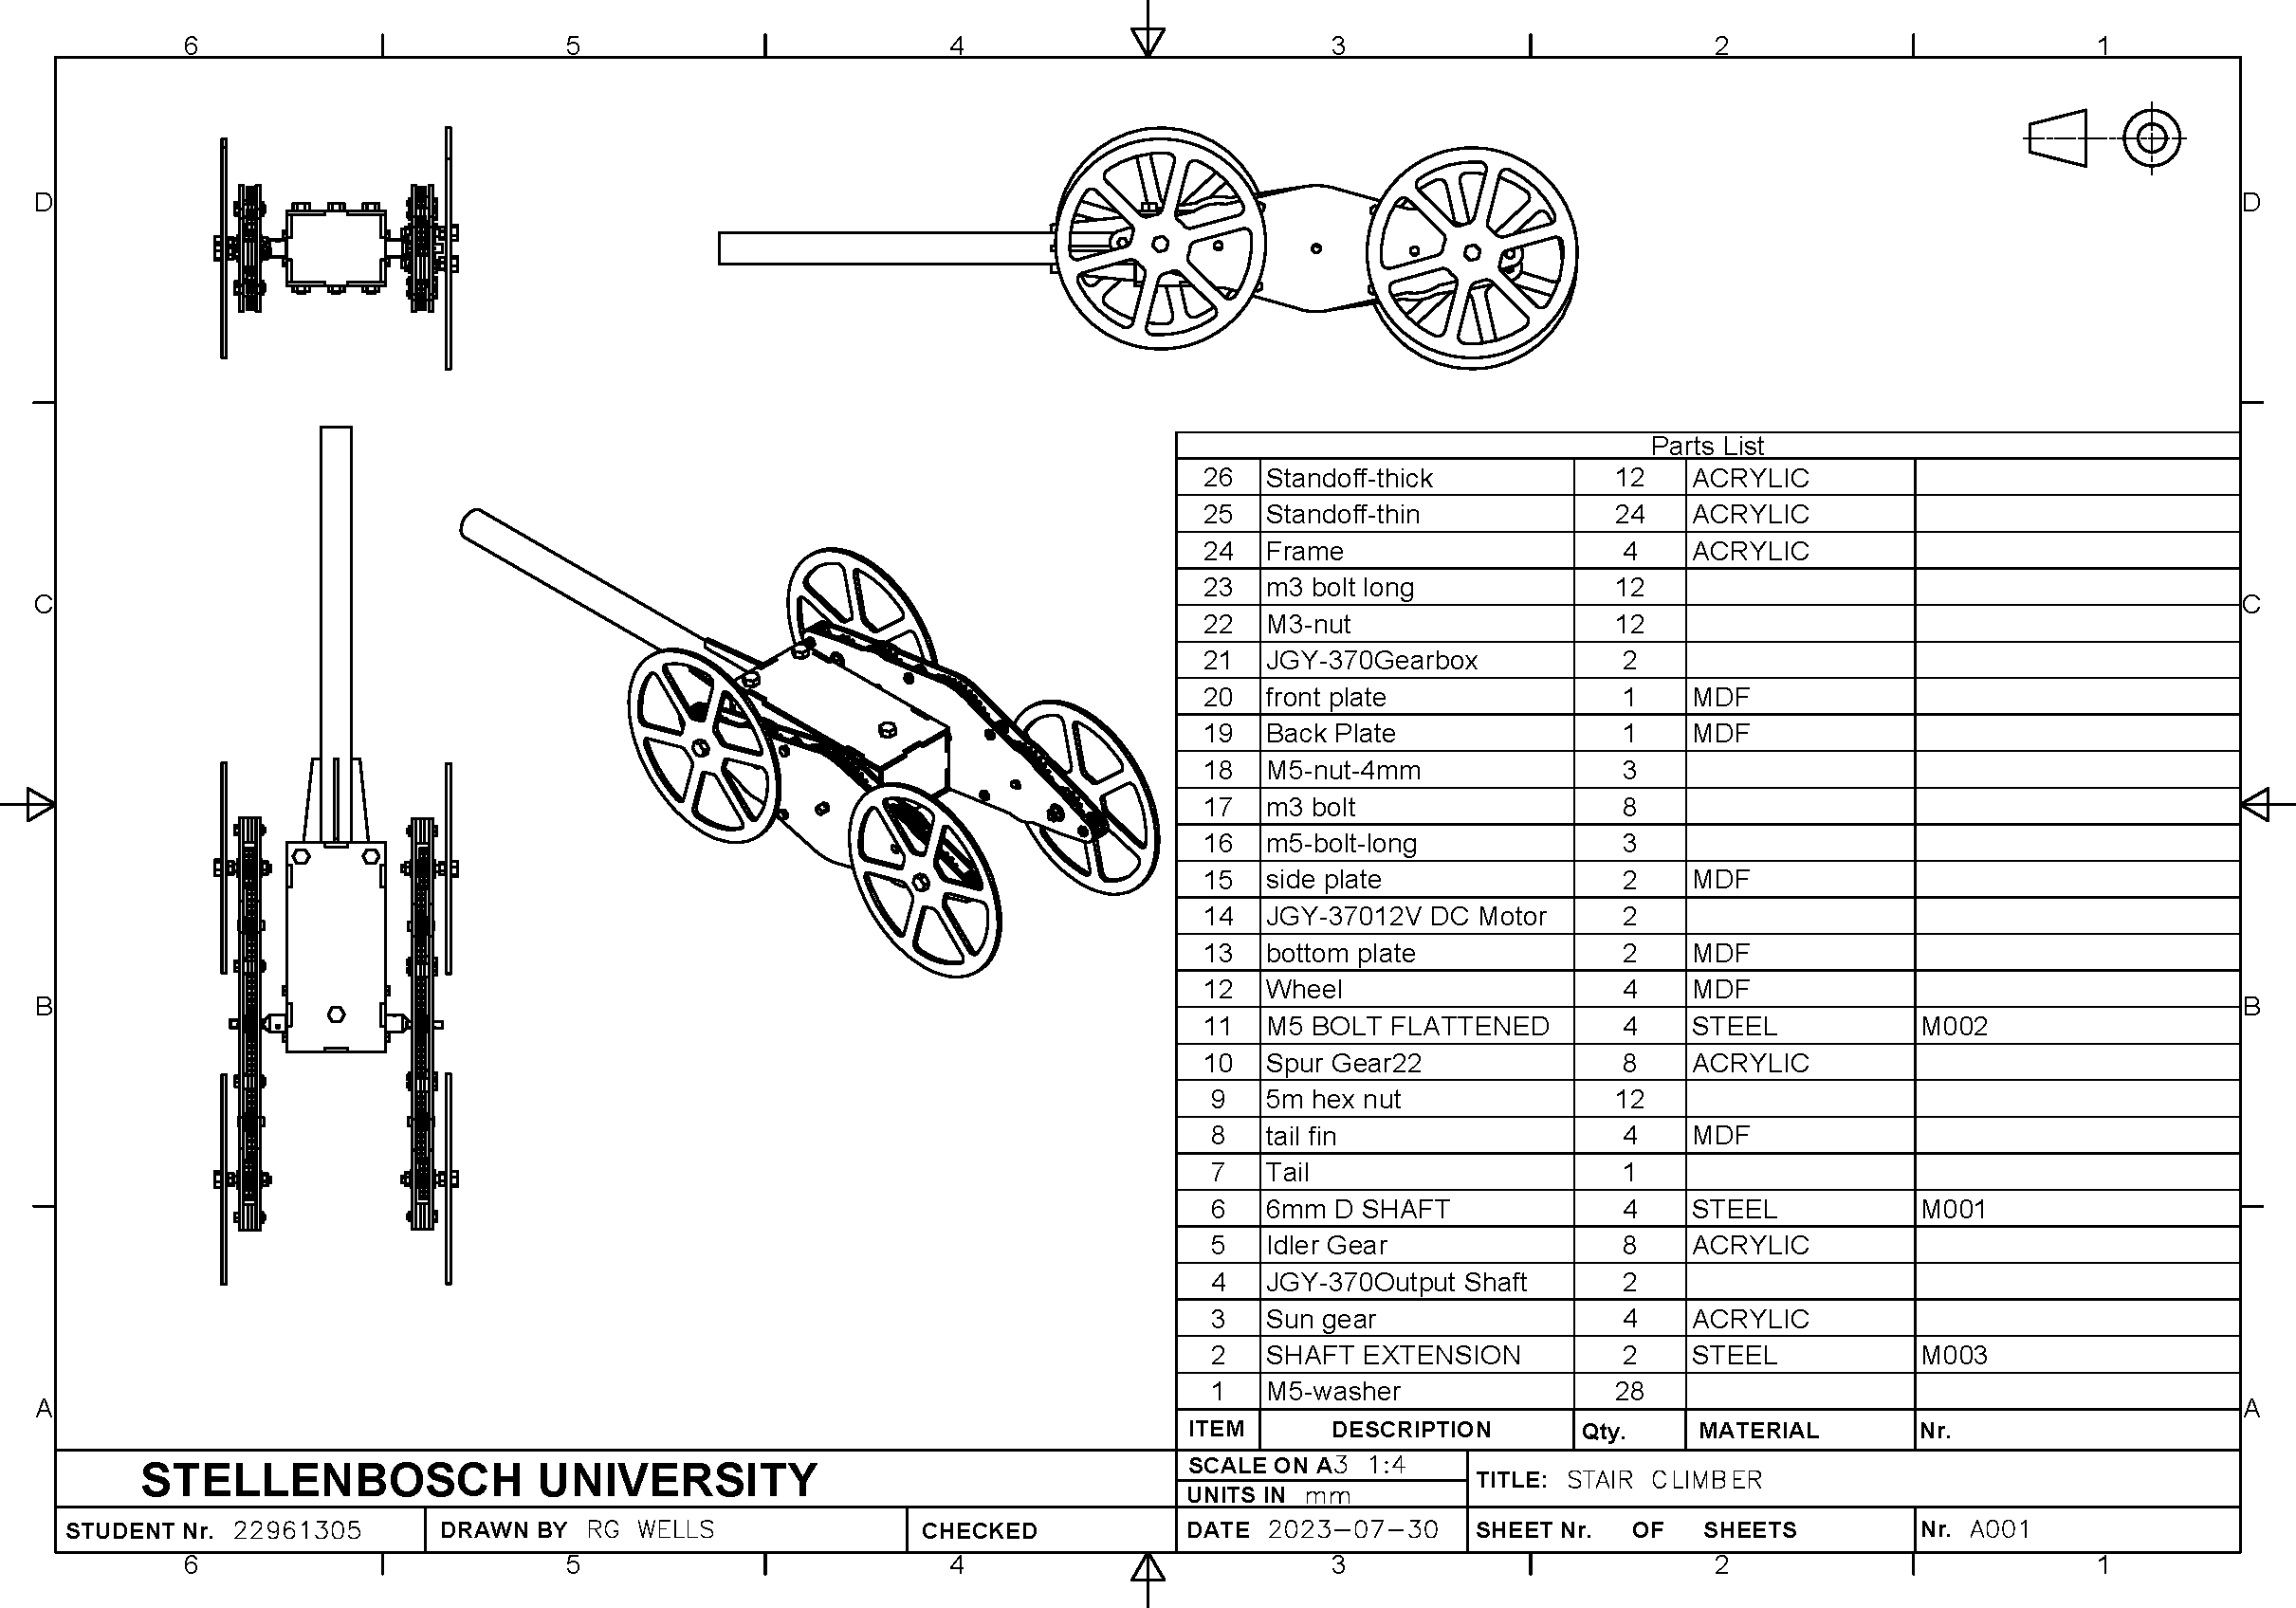
\includepdf[pages=-, fitpaper]{chaps-append/STAIR-CLIMBER.pdf}


%\clearpage%\KOMAoptions{paper=A4,paper=portrait, pagesize}
%\recalctypearea
%\chapter{Experiment}

In order to validate that the model is accurate for each motion, the torque that causes the device to perform each motion determined experimentally. The equivalent values produced by the model can be compared with the measured torques to validate the model quantitatively. However, the torque produced by a DC motor cannot be measured or set directly. The torque of a DC motor is proportional to the current running through it, and when the motor isn't moving, the current is proportional to the voltage across the motor terminals. The terminal voltage is varied in this experiment.

\section{Voltage-torque calibration}
The relationship between terminal voltage and stalling torque is determined experimentally, this will allow subsequent experiments to measure the terminal voltage and calculate the stalling torque.
To characterise the motors, an experiment was set up to determine the stalling torque produced at different input voltages. In this experiment, a the motor lifts a lever with a mass attached. The torque required to lift the lever increases as the lever angle increases, until the motor can no longer provide enough torque and stalls. The lever angle which causes the motor to stall can be used to calculate the stalling torque, specifically by using the horizontal displacement of the mass,
\begin{equation}
	T_{Stall} = m g s_x
\end{equation}
where $T_{Stall}$ is the stalling torque, $m$ is the mass attached to the lever, $g$ is the gravitational acceleration, and $s_x$ is the horizontal displacement between the mass and the motor axis.
%figure here ????
This test is repeated with different motor voltages.\\

\subsection{Variables}
Independent variable:\\
$\bullet$ Motor voltage (V)\\
Dependent variable:\\
$\bullet$ Distance the weight is lifted (mm)\\
Controlled variables:\\
$\bullet$ Motor used\\
$\bullet$ Lever used\\
$\bullet$ Power supply used\\
$\bullet$ Multimeter used\\
$\bullet$ Ruler used\\

\subsection{Method}

\begin{enumerate}
	\item Remove LIM from motor axle.
	\item Attach the lever to the motor axle.
	\item Measure the weight of the mass on a calibrated scale. \label{stepMeasure}
	\item Drive the motor until the lever is pointing straight down.
	\item Attach the mass to the lever.
	\item Adjust the voltage of the power supply to the chosen value. \label{stepAdjust}
	\item Power on the motor.
	\item Wait until the lever stops moving.
	\item Record the voltage across the motor terminals. 
	\item Quickly power off the motor. Leaving the motor on while stalling can cause damage to the motor.
	\item Measure the horizontal distance that the lever has moved.
	\item Drive the motor until the lever is pointing straight down. \label{stepReset}
	\item Repeat steps \ref{stepAdjust} to \ref{stepReset} with different power supply voltages.
	\item Remove the mass from the lever. \label{stepRemove}
	\item Repeat steps \ref{stepMeasure} to \ref{stepRemove} with different masses.
\end{enumerate}
\subsection{Results}
The measured results, as well as the calculated torque, are shown in Table \ref{voltage-torque-table}, and visualised in Figure \ref{torque-voltage-plot}.

\begin{table}[!ht]
	\label{voltage-torque-table}
	\centering
	\begin{tabular}{|l|l|l|l|}
		\hline
		Mass (g) & Lever (mm) & Voltage (V) & Torque (Nm) \\ \hline
		145 & 97 & 0.83 & 0.13797765 \\ \hline
		145 & 101 & 0.92 & 0.14366745 \\ \hline
		145 & 151 & 1.1 & 0.21478995 \\ \hline
		204 & 154 & 1.22 & 0.30819096 \\ \hline
		204 & 229 & 1.56 & 0.45828396 \\ \hline
		542 & 89 & 1.72 & 0.47321478 \\ \hline
		537 & 106 & 1.93 & 0.55840482 \\ \hline
		542 & 106 & 1.8 & 0.56360412 \\ \hline
		537 & 164 & 2.45 & 0.86394708 \\ \hline
		542 & 171 & 2.5 & 0.90921042 \\ \hline
		542 & 220 & 3 & 1.1697444 \\ \hline
		542 & 242 & 3.25 & 1.28671884 \\ \hline
		1289 & 117 & 3.5 & 1.47947553 \\ \hline
		1289 & 136 & 4 & 1.71973224 \\ \hline
		1289 & 160 & 4.5 & 2.0232144 \\ \hline
	\end{tabular}
\end{table}

\begin{figure}[!h]
	\centering
	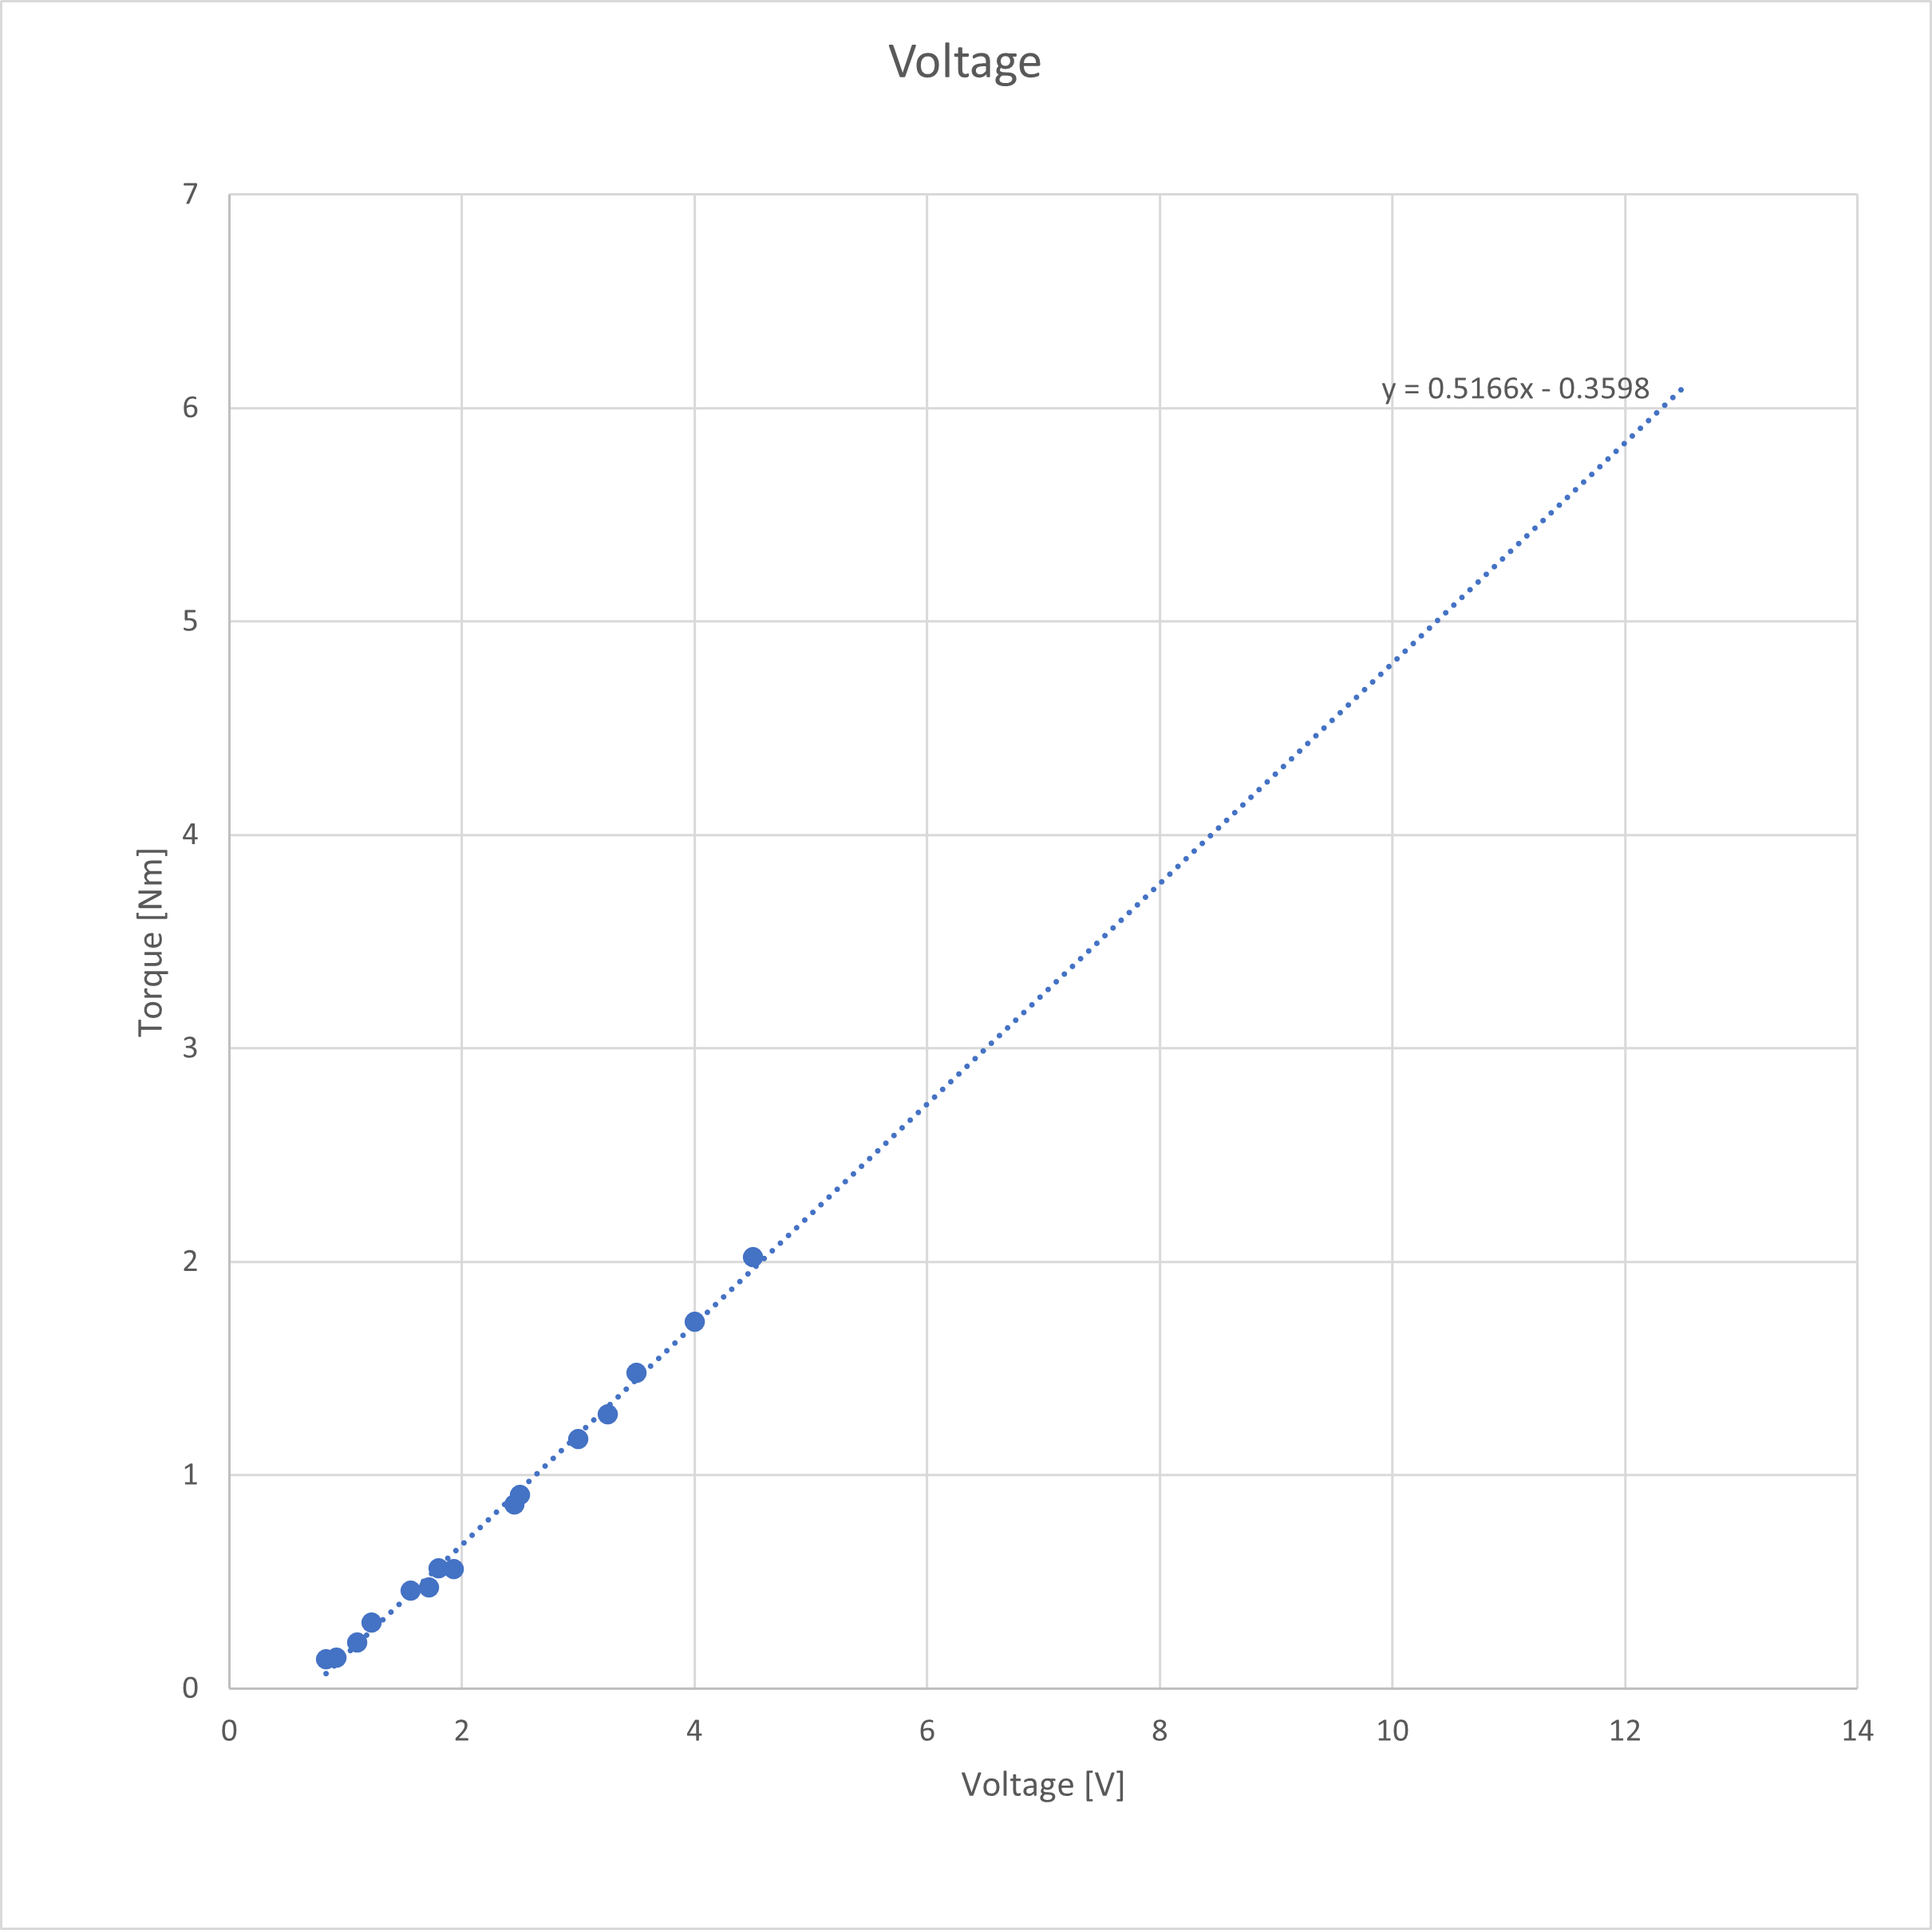
\includegraphics[width=0.8\textwidth]{plots/torque-voltage-relation.png}
	\caption{Relationship between motor voltage and stalling torque.}
	\label{torque-voltage-plot}
\end{figure}

This plot shows a linear relationship between stalling torque and voltage, and gives the formula,
\begin{equation}
	T_{Stall} =  0.5166 V - 0.3598 \label{eqTorqueVoltage}
\end{equation}
where $V$ is the motor terminal voltage.
This experiment did not attempt to measure torques beyond $2 Nm$ as this risked damaging the device and was beyond the expected requirements for the device.



\section{Climbing torque}
This experiment aims to determine the torque required to lift the device through each stage of motion. The results of this experiment will be compared with the compared with the theoretical torques required provided by the model and the simulation. The device is placed in the starting position for each stage of motion and powered with a certain supply voltage. The motion of the device is then assessed, if the device does not move then it is marked as "None"; if the device starts to move but does not complete the stage of motion, it is marked as "Partial"; and if it completes the stage of motion, it is marked as "Full".\\

%???? figure here

\subsection{Variables}
Independent variable:\\
$\bullet$ Motor voltage (V)\\
Dependent variable:\\
$\bullet$ Assessment of motion ("Full", "Partial", or "None")\\
Controlled variables:\\
$\bullet$ LIMed device\\
$\bullet$ Stairs\\
$\bullet$ Multimeter used\\


\subsection{Method}

\begin{enumerate}
	\item Place device in the starting position for the chosen stage of motion. \label{stepPlace}
	\item Adjust the voltage of the power supply to the chosen value.
	\item Power on the device.
	\item Observe how the device moves and classify the movement into "Full", "Partial", or "None". 
	\item Record the voltage across the motor terminals. 
	\item Power off the device.\label{stepOff}
	\item Repeat steps \ref{stepPlace} to \ref{stepOff} with a range of power supply voltages.\label{stepRepeatVoltage}
	\item Repeat steps \ref{stepPlace} to \ref{stepRepeatVoltage} for the different stages of motion.
\end{enumerate}

\subsection{Results}

Table \ref{tableStage1Torque} shows the measured results for the Stage 1 motion, as well as the torques calculated using Equation \ref{eqTorqueVoltage}. The data for the other stages of motion can be found in Appendix ???.

\begin{table}[!h]
	\caption{Torque experiment results for Stage 1}
	\label{tableStage1Torque}
	\centering
	\begin{tabular}{|l|l|l|}
		\hline
		Voltage (V) & Assessment of motion & Torque (Nm) \\ \hline
		0.89 & None & 0.099974 \\ \hline
		1.08 & None & 0.198128 \\ \hline
		1.12 & None & 0.218792 \\ \hline
		1.57 & None & 0.451262 \\ \hline
		1.68 & None & 0.508088 \\ \hline
		1.74 & None & 0.539084 \\ \hline
		1.81 & None & 0.575246 \\ \hline
		1.87 & None & 0.606242 \\ \hline
		1.89 & Partial & 0.616574 \\ \hline
		1.98 & Partial & 0.663068 \\ \hline
		2.05 & Partial & 0.69923 \\ \hline
		2.11 & Full & 0.730226 \\ \hline
		2.13 & Full & 0.740558 \\ \hline
		2.25 & Full & 0.80255 \\ \hline
		2.26 & Full & 0.807716 \\ \hline
		2.3 & Full & 0.82838 \\ \hline
	\end{tabular}
\end{table}

This data is plotted in Figure \ref{plotassessment-torque-relation-stage1}, which shows that the full motion only happens with torques of at least $0.73 Nm$, while partial motion only requires $0.61 Nm$.

\begin{figure}[h]
	\centering
	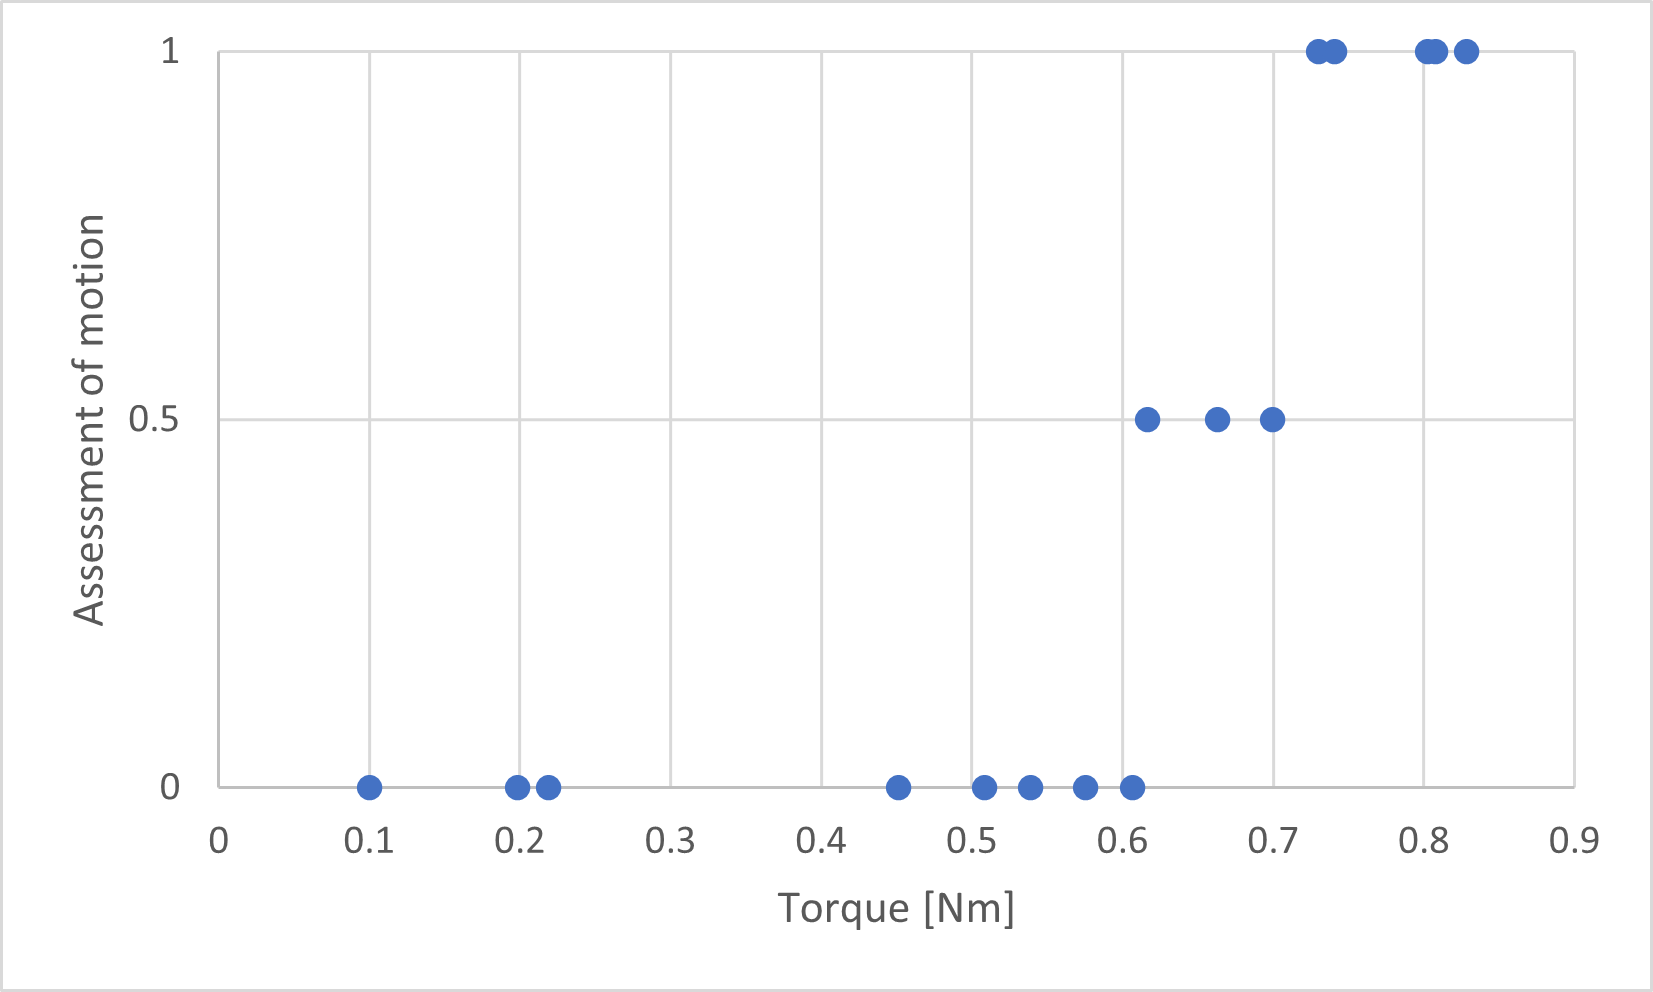
\includegraphics[width=0.8\textwidth]{plots/assessment-torque-relation-stage1}
	\caption{Relationship between torque and motion for Stage 1, with 0, 0.5, and 1 representing "None", "Partial", and "Full" respectively.}
	\label{plotassessment-torque-relation-stage1}
\end{figure}




\backmatter%----------------------------------------------------------
\bibliography{bib/bib-sample}
 
\end{document}   

